\documentclass[twoside]{book}

% Packages required by doxygen
\usepackage{fixltx2e}
\usepackage{calc}
\usepackage{doxygen}
\usepackage[export]{adjustbox} % also loads graphicx
\usepackage{graphicx}
\usepackage[utf8]{inputenc}
\usepackage{makeidx}
\usepackage{multicol}
\usepackage{multirow}
\PassOptionsToPackage{warn}{textcomp}
\usepackage{textcomp}
\usepackage[nointegrals]{wasysym}
\usepackage[table]{xcolor}

% Font selection
\usepackage[T1]{fontenc}
\usepackage[scaled=.90]{helvet}
\usepackage{courier}
\usepackage{amssymb}
\usepackage{sectsty}
\renewcommand{\familydefault}{\sfdefault}
\allsectionsfont{%
  \fontseries{bc}\selectfont%
  \color{darkgray}%
}
\renewcommand{\DoxyLabelFont}{%
  \fontseries{bc}\selectfont%
  \color{darkgray}%
}
\newcommand{\+}{\discretionary{\mbox{\scriptsize$\hookleftarrow$}}{}{}}

% Page & text layout
\usepackage{geometry}
\geometry{%
  a4paper,%
  top=2.5cm,%
  bottom=2.5cm,%
  left=2.5cm,%
  right=2.5cm%
}
\tolerance=750
\hfuzz=15pt
\hbadness=750
\setlength{\emergencystretch}{15pt}
\setlength{\parindent}{0cm}
\setlength{\parskip}{3ex plus 2ex minus 2ex}
\makeatletter
\renewcommand{\paragraph}{%
  \@startsection{paragraph}{4}{0ex}{-1.0ex}{1.0ex}{%
    \normalfont\normalsize\bfseries\SS@parafont%
  }%
}
\renewcommand{\subparagraph}{%
  \@startsection{subparagraph}{5}{0ex}{-1.0ex}{1.0ex}{%
    \normalfont\normalsize\bfseries\SS@subparafont%
  }%
}
\makeatother

% Headers & footers
\usepackage{fancyhdr}
\pagestyle{fancyplain}
\fancyhead[LE]{\fancyplain{}{\bfseries\thepage}}
\fancyhead[CE]{\fancyplain{}{}}
\fancyhead[RE]{\fancyplain{}{\bfseries\leftmark}}
\fancyhead[LO]{\fancyplain{}{\bfseries\rightmark}}
\fancyhead[CO]{\fancyplain{}{}}
\fancyhead[RO]{\fancyplain{}{\bfseries\thepage}}
\fancyfoot[LE]{\fancyplain{}{}}
\fancyfoot[CE]{\fancyplain{}{}}
\fancyfoot[RE]{\fancyplain{}{\bfseries\scriptsize 制作者 Doxygen }}
\fancyfoot[LO]{\fancyplain{}{\bfseries\scriptsize 制作者 Doxygen }}
\fancyfoot[CO]{\fancyplain{}{}}
\fancyfoot[RO]{\fancyplain{}{}}
\renewcommand{\footrulewidth}{0.4pt}
\renewcommand{\chaptermark}[1]{%
  \markboth{#1}{}%
}
\renewcommand{\sectionmark}[1]{%
  \markright{\thesection\ #1}%
}

% Indices & bibliography
\usepackage{natbib}
\usepackage[titles]{tocloft}
\setcounter{tocdepth}{3}
\setcounter{secnumdepth}{5}
\makeindex

% Hyperlinks (required, but should be loaded last)
\usepackage{ifpdf}
\ifpdf
  \usepackage[pdftex,pagebackref=true]{hyperref}
\else
  \usepackage[ps2pdf,pagebackref=true]{hyperref}
\fi
\hypersetup{%
  colorlinks=true,%
  linkcolor=blue,%
  citecolor=blue,%
  unicode%
}

% Custom commands
\newcommand{\clearemptydoublepage}{%
  \newpage{\pagestyle{empty}\cleardoublepage}%
}

\usepackage{caption}
\captionsetup{labelsep=space,justification=centering,font={bf},singlelinecheck=off,skip=4pt,position=top}

%===== C O N T E N T S =====

\begin{document}

% Titlepage & ToC
\hypersetup{pageanchor=false,
             bookmarksnumbered=true,
             pdfencoding=unicode
            }
\pagenumbering{roman}
\begin{titlepage}
\vspace*{7cm}
\begin{center}%
{\Large My Project }\\
\vspace*{1cm}
{\large 制作者 Doxygen 1.8.11}\\
\end{center}
\end{titlepage}
\clearemptydoublepage
\tableofcontents
\clearemptydoublepage
\pagenumbering{arabic}
\hypersetup{pageanchor=true}

%--- Begin generated contents ---
\chapter{继承关系索引}
\section{类继承关系}
此继承关系列表按字典顺序粗略的排序\+: \begin{DoxyCompactList}
\item \contentsline{section}{\+\_\+\+U\+S\+B2089\+\_\+\+P\+A\+R\+A\+\_\+\+AD}{\pageref{struct___u_s_b2089___p_a_r_a___a_d}}{}
\item Q\+Object\begin{DoxyCompactList}
\item \contentsline{section}{D\+AC}{\pageref{class_d_a_c}}{}
\item \contentsline{section}{D\+A\+Parameters}{\pageref{class_d_a_parameters}}{}
\item \contentsline{section}{D\+AQ}{\pageref{class_d_a_q}}{}
\item \contentsline{section}{Database}{\pageref{class_database}}{}
\item \contentsline{section}{Data\+Source}{\pageref{class_data_source}}{}
\item \contentsline{section}{D\+B\+Worker}{\pageref{class_d_b_worker}}{}
\item \contentsline{section}{Device}{\pageref{class_device}}{}
\item \contentsline{section}{Gas\+Data}{\pageref{class_gas_data}}{}
\item \contentsline{section}{Serial}{\pageref{class_serial}}{}
\item \contentsline{section}{Timer}{\pageref{class_timer}}{}
\end{DoxyCompactList}
\end{DoxyCompactList}

\chapter{类索引}
\section{类列表}
这里列出了所有类、结构、联合以及接口定义等,并附带简要说明\+:\begin{DoxyCompactList}
\item\contentsline{section}{\hyperlink{struct___u_s_b2089___p_a_r_a___a_d}{\+\_\+\+U\+S\+B2089\+\_\+\+P\+A\+R\+A\+\_\+\+AD} }{\pageref{struct___u_s_b2089___p_a_r_a___a_d}}{}
\item\contentsline{section}{\hyperlink{class_d_a_c}{D\+AC} }{\pageref{class_d_a_c}}{}
\item\contentsline{section}{\hyperlink{class_d_a_parameters}{D\+A\+Parameters} }{\pageref{class_d_a_parameters}}{}
\item\contentsline{section}{\hyperlink{class_d_a_q}{D\+AQ} }{\pageref{class_d_a_q}}{}
\item\contentsline{section}{\hyperlink{class_database}{Database} }{\pageref{class_database}}{}
\item\contentsline{section}{\hyperlink{class_data_source}{Data\+Source} }{\pageref{class_data_source}}{}
\item\contentsline{section}{\hyperlink{class_d_b_worker}{D\+B\+Worker} }{\pageref{class_d_b_worker}}{}
\item\contentsline{section}{\hyperlink{class_device}{Device} }{\pageref{class_device}}{}
\item\contentsline{section}{\hyperlink{class_gas_data}{Gas\+Data} }{\pageref{class_gas_data}}{}
\item\contentsline{section}{\hyperlink{class_serial}{Serial} }{\pageref{class_serial}}{}
\item\contentsline{section}{\hyperlink{class_timer}{Timer} }{\pageref{class_timer}}{}
\end{DoxyCompactList}

\chapter{文件索引}
\section{文件列表}
这里列出了所有文件,并附带简要说明\+:\begin{DoxyCompactList}
\item\contentsline{section}{\hyperlink{dac_8cpp}{dac.\+cpp} }{\pageref{dac_8cpp}}{}
\item\contentsline{section}{\hyperlink{dac_8h}{dac.\+h} }{\pageref{dac_8h}}{}
\item\contentsline{section}{\hyperlink{daparameters_8cpp}{daparameters.\+cpp} }{\pageref{daparameters_8cpp}}{}
\item\contentsline{section}{\hyperlink{daparameters_8h}{daparameters.\+h} }{\pageref{daparameters_8h}}{}
\item\contentsline{section}{\hyperlink{daq_8cpp}{daq.\+cpp} }{\pageref{daq_8cpp}}{}
\item\contentsline{section}{\hyperlink{daq_8h}{daq.\+h} }{\pageref{daq_8h}}{}
\item\contentsline{section}{\hyperlink{database_8cpp}{database.\+cpp} }{\pageref{database_8cpp}}{}
\item\contentsline{section}{\hyperlink{database_8h}{database.\+h} }{\pageref{database_8h}}{}
\item\contentsline{section}{\hyperlink{datasource_8cpp}{datasource.\+cpp} }{\pageref{datasource_8cpp}}{}
\item\contentsline{section}{\hyperlink{datasource_8h}{datasource.\+h} }{\pageref{datasource_8h}}{}
\item\contentsline{section}{\hyperlink{device_8cpp}{device.\+cpp} }{\pageref{device_8cpp}}{}
\item\contentsline{section}{\hyperlink{device_8h}{device.\+h} }{\pageref{device_8h}}{}
\item\contentsline{section}{\hyperlink{gasdata_8cpp}{gasdata.\+cpp} }{\pageref{gasdata_8cpp}}{}
\item\contentsline{section}{\hyperlink{gasdata_8h}{gasdata.\+h} }{\pageref{gasdata_8h}}{}
\item\contentsline{section}{\hyperlink{main_8cpp}{main.\+cpp} }{\pageref{main_8cpp}}{}
\item\contentsline{section}{\hyperlink{serial_8cpp}{serial.\+cpp} }{\pageref{serial_8cpp}}{}
\item\contentsline{section}{\hyperlink{serial_8h}{serial.\+h} }{\pageref{serial_8h}}{}
\item\contentsline{section}{\hyperlink{timer_8cpp}{timer.\+cpp} }{\pageref{timer_8cpp}}{}
\item\contentsline{section}{\hyperlink{timer_8h}{timer.\+h} }{\pageref{timer_8h}}{}
\item\contentsline{section}{\hyperlink{usb2089_8h}{usb2089.\+h} }{\pageref{usb2089_8h}}{}
\end{DoxyCompactList}

\chapter{类说明}
\hypertarget{struct___u_s_b2089___p_a_r_a___a_d}{}\section{\+\_\+\+U\+S\+B2089\+\_\+\+P\+A\+R\+A\+\_\+\+A\+D结构体 参考}
\label{struct___u_s_b2089___p_a_r_a___a_d}\index{\+\_\+\+U\+S\+B2089\+\_\+\+P\+A\+R\+A\+\_\+\+AD@{\+\_\+\+U\+S\+B2089\+\_\+\+P\+A\+R\+A\+\_\+\+AD}}


{\ttfamily \#include $<$usb2089.\+h$>$}



\+\_\+\+U\+S\+B2089\+\_\+\+P\+A\+R\+A\+\_\+\+AD 的协作图\+:
\nopagebreak
\begin{figure}[H]
\begin{center}
\leavevmode
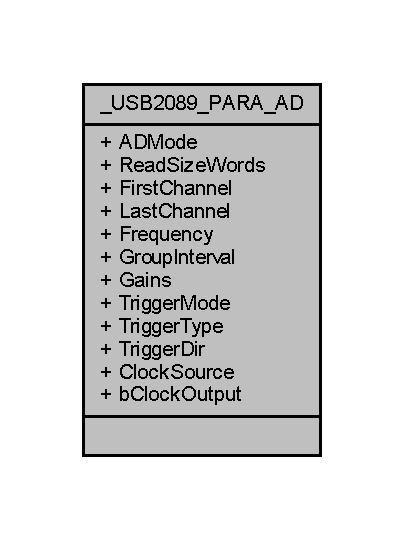
\includegraphics[width=194pt]{struct___u_s_b2089___p_a_r_a___a_d__coll__graph}
\end{center}
\end{figure}
\subsection*{Public 属性}
\begin{DoxyCompactItemize}
\item 
L\+O\+NG \hyperlink{struct___u_s_b2089___p_a_r_a___a_d_a8e4e21c70f5f392b71a111a3df90deb1}{A\+D\+Mode}
\item 
L\+O\+NG \hyperlink{struct___u_s_b2089___p_a_r_a___a_d_ad337e2c8a8ab80adf0721f273af39b5b}{Read\+Size\+Words}
\item 
L\+O\+NG \hyperlink{struct___u_s_b2089___p_a_r_a___a_d_a37a8a439bcde128816b7f9bb206f9906}{First\+Channel}
\item 
L\+O\+NG \hyperlink{struct___u_s_b2089___p_a_r_a___a_d_a5e53b9537aad636c0e28c20ffe944814}{Last\+Channel}
\item 
L\+O\+NG \hyperlink{struct___u_s_b2089___p_a_r_a___a_d_a214d91a7b62122358aee9225ef604369}{Frequency}
\item 
L\+O\+NG \hyperlink{struct___u_s_b2089___p_a_r_a___a_d_a90588f72e8d53708e73c7d806f990d4f}{Group\+Interval}
\item 
L\+O\+NG \hyperlink{struct___u_s_b2089___p_a_r_a___a_d_a940668fdf91fa5d30cbb76e3c2af632f}{Gains}
\item 
L\+O\+NG \hyperlink{struct___u_s_b2089___p_a_r_a___a_d_a21784127891ec6b61e1c540eeeebbdf8}{Trigger\+Mode}
\item 
L\+O\+NG \hyperlink{struct___u_s_b2089___p_a_r_a___a_d_a40a568ec452439655638e36c8b11c438}{Trigger\+Type}
\item 
L\+O\+NG \hyperlink{struct___u_s_b2089___p_a_r_a___a_d_a7e2a33fc23abe47b91154e556e85c991}{Trigger\+Dir}
\item 
L\+O\+NG \hyperlink{struct___u_s_b2089___p_a_r_a___a_d_a61fb08b66760f8d2a26b9d0514ef2040}{Clock\+Source}
\item 
L\+O\+NG \hyperlink{struct___u_s_b2089___p_a_r_a___a_d_ad1f0e7462f81ac385fa36525160ba3a5}{b\+Clock\+Output}
\end{DoxyCompactItemize}


\subsection{类成员变量说明}
\index{\+\_\+\+U\+S\+B2089\+\_\+\+P\+A\+R\+A\+\_\+\+AD@{\+\_\+\+U\+S\+B2089\+\_\+\+P\+A\+R\+A\+\_\+\+AD}!A\+D\+Mode@{A\+D\+Mode}}
\index{A\+D\+Mode@{A\+D\+Mode}!\+\_\+\+U\+S\+B2089\+\_\+\+P\+A\+R\+A\+\_\+\+AD@{\+\_\+\+U\+S\+B2089\+\_\+\+P\+A\+R\+A\+\_\+\+AD}}
\subsubsection[{\texorpdfstring{A\+D\+Mode}{ADMode}}]{\setlength{\rightskip}{0pt plus 5cm}L\+O\+NG \+\_\+\+U\+S\+B2089\+\_\+\+P\+A\+R\+A\+\_\+\+A\+D\+::\+A\+D\+Mode}\hypertarget{struct___u_s_b2089___p_a_r_a___a_d_a8e4e21c70f5f392b71a111a3df90deb1}{}\label{struct___u_s_b2089___p_a_r_a___a_d_a8e4e21c70f5f392b71a111a3df90deb1}
\index{\+\_\+\+U\+S\+B2089\+\_\+\+P\+A\+R\+A\+\_\+\+AD@{\+\_\+\+U\+S\+B2089\+\_\+\+P\+A\+R\+A\+\_\+\+AD}!b\+Clock\+Output@{b\+Clock\+Output}}
\index{b\+Clock\+Output@{b\+Clock\+Output}!\+\_\+\+U\+S\+B2089\+\_\+\+P\+A\+R\+A\+\_\+\+AD@{\+\_\+\+U\+S\+B2089\+\_\+\+P\+A\+R\+A\+\_\+\+AD}}
\subsubsection[{\texorpdfstring{b\+Clock\+Output}{bClockOutput}}]{\setlength{\rightskip}{0pt plus 5cm}L\+O\+NG \+\_\+\+U\+S\+B2089\+\_\+\+P\+A\+R\+A\+\_\+\+A\+D\+::b\+Clock\+Output}\hypertarget{struct___u_s_b2089___p_a_r_a___a_d_ad1f0e7462f81ac385fa36525160ba3a5}{}\label{struct___u_s_b2089___p_a_r_a___a_d_ad1f0e7462f81ac385fa36525160ba3a5}
\index{\+\_\+\+U\+S\+B2089\+\_\+\+P\+A\+R\+A\+\_\+\+AD@{\+\_\+\+U\+S\+B2089\+\_\+\+P\+A\+R\+A\+\_\+\+AD}!Clock\+Source@{Clock\+Source}}
\index{Clock\+Source@{Clock\+Source}!\+\_\+\+U\+S\+B2089\+\_\+\+P\+A\+R\+A\+\_\+\+AD@{\+\_\+\+U\+S\+B2089\+\_\+\+P\+A\+R\+A\+\_\+\+AD}}
\subsubsection[{\texorpdfstring{Clock\+Source}{ClockSource}}]{\setlength{\rightskip}{0pt plus 5cm}L\+O\+NG \+\_\+\+U\+S\+B2089\+\_\+\+P\+A\+R\+A\+\_\+\+A\+D\+::\+Clock\+Source}\hypertarget{struct___u_s_b2089___p_a_r_a___a_d_a61fb08b66760f8d2a26b9d0514ef2040}{}\label{struct___u_s_b2089___p_a_r_a___a_d_a61fb08b66760f8d2a26b9d0514ef2040}
\index{\+\_\+\+U\+S\+B2089\+\_\+\+P\+A\+R\+A\+\_\+\+AD@{\+\_\+\+U\+S\+B2089\+\_\+\+P\+A\+R\+A\+\_\+\+AD}!First\+Channel@{First\+Channel}}
\index{First\+Channel@{First\+Channel}!\+\_\+\+U\+S\+B2089\+\_\+\+P\+A\+R\+A\+\_\+\+AD@{\+\_\+\+U\+S\+B2089\+\_\+\+P\+A\+R\+A\+\_\+\+AD}}
\subsubsection[{\texorpdfstring{First\+Channel}{FirstChannel}}]{\setlength{\rightskip}{0pt plus 5cm}L\+O\+NG \+\_\+\+U\+S\+B2089\+\_\+\+P\+A\+R\+A\+\_\+\+A\+D\+::\+First\+Channel}\hypertarget{struct___u_s_b2089___p_a_r_a___a_d_a37a8a439bcde128816b7f9bb206f9906}{}\label{struct___u_s_b2089___p_a_r_a___a_d_a37a8a439bcde128816b7f9bb206f9906}
\index{\+\_\+\+U\+S\+B2089\+\_\+\+P\+A\+R\+A\+\_\+\+AD@{\+\_\+\+U\+S\+B2089\+\_\+\+P\+A\+R\+A\+\_\+\+AD}!Frequency@{Frequency}}
\index{Frequency@{Frequency}!\+\_\+\+U\+S\+B2089\+\_\+\+P\+A\+R\+A\+\_\+\+AD@{\+\_\+\+U\+S\+B2089\+\_\+\+P\+A\+R\+A\+\_\+\+AD}}
\subsubsection[{\texorpdfstring{Frequency}{Frequency}}]{\setlength{\rightskip}{0pt plus 5cm}L\+O\+NG \+\_\+\+U\+S\+B2089\+\_\+\+P\+A\+R\+A\+\_\+\+A\+D\+::\+Frequency}\hypertarget{struct___u_s_b2089___p_a_r_a___a_d_a214d91a7b62122358aee9225ef604369}{}\label{struct___u_s_b2089___p_a_r_a___a_d_a214d91a7b62122358aee9225ef604369}
\index{\+\_\+\+U\+S\+B2089\+\_\+\+P\+A\+R\+A\+\_\+\+AD@{\+\_\+\+U\+S\+B2089\+\_\+\+P\+A\+R\+A\+\_\+\+AD}!Gains@{Gains}}
\index{Gains@{Gains}!\+\_\+\+U\+S\+B2089\+\_\+\+P\+A\+R\+A\+\_\+\+AD@{\+\_\+\+U\+S\+B2089\+\_\+\+P\+A\+R\+A\+\_\+\+AD}}
\subsubsection[{\texorpdfstring{Gains}{Gains}}]{\setlength{\rightskip}{0pt plus 5cm}L\+O\+NG \+\_\+\+U\+S\+B2089\+\_\+\+P\+A\+R\+A\+\_\+\+A\+D\+::\+Gains}\hypertarget{struct___u_s_b2089___p_a_r_a___a_d_a940668fdf91fa5d30cbb76e3c2af632f}{}\label{struct___u_s_b2089___p_a_r_a___a_d_a940668fdf91fa5d30cbb76e3c2af632f}
\index{\+\_\+\+U\+S\+B2089\+\_\+\+P\+A\+R\+A\+\_\+\+AD@{\+\_\+\+U\+S\+B2089\+\_\+\+P\+A\+R\+A\+\_\+\+AD}!Group\+Interval@{Group\+Interval}}
\index{Group\+Interval@{Group\+Interval}!\+\_\+\+U\+S\+B2089\+\_\+\+P\+A\+R\+A\+\_\+\+AD@{\+\_\+\+U\+S\+B2089\+\_\+\+P\+A\+R\+A\+\_\+\+AD}}
\subsubsection[{\texorpdfstring{Group\+Interval}{GroupInterval}}]{\setlength{\rightskip}{0pt plus 5cm}L\+O\+NG \+\_\+\+U\+S\+B2089\+\_\+\+P\+A\+R\+A\+\_\+\+A\+D\+::\+Group\+Interval}\hypertarget{struct___u_s_b2089___p_a_r_a___a_d_a90588f72e8d53708e73c7d806f990d4f}{}\label{struct___u_s_b2089___p_a_r_a___a_d_a90588f72e8d53708e73c7d806f990d4f}
\index{\+\_\+\+U\+S\+B2089\+\_\+\+P\+A\+R\+A\+\_\+\+AD@{\+\_\+\+U\+S\+B2089\+\_\+\+P\+A\+R\+A\+\_\+\+AD}!Last\+Channel@{Last\+Channel}}
\index{Last\+Channel@{Last\+Channel}!\+\_\+\+U\+S\+B2089\+\_\+\+P\+A\+R\+A\+\_\+\+AD@{\+\_\+\+U\+S\+B2089\+\_\+\+P\+A\+R\+A\+\_\+\+AD}}
\subsubsection[{\texorpdfstring{Last\+Channel}{LastChannel}}]{\setlength{\rightskip}{0pt plus 5cm}L\+O\+NG \+\_\+\+U\+S\+B2089\+\_\+\+P\+A\+R\+A\+\_\+\+A\+D\+::\+Last\+Channel}\hypertarget{struct___u_s_b2089___p_a_r_a___a_d_a5e53b9537aad636c0e28c20ffe944814}{}\label{struct___u_s_b2089___p_a_r_a___a_d_a5e53b9537aad636c0e28c20ffe944814}
\index{\+\_\+\+U\+S\+B2089\+\_\+\+P\+A\+R\+A\+\_\+\+AD@{\+\_\+\+U\+S\+B2089\+\_\+\+P\+A\+R\+A\+\_\+\+AD}!Read\+Size\+Words@{Read\+Size\+Words}}
\index{Read\+Size\+Words@{Read\+Size\+Words}!\+\_\+\+U\+S\+B2089\+\_\+\+P\+A\+R\+A\+\_\+\+AD@{\+\_\+\+U\+S\+B2089\+\_\+\+P\+A\+R\+A\+\_\+\+AD}}
\subsubsection[{\texorpdfstring{Read\+Size\+Words}{ReadSizeWords}}]{\setlength{\rightskip}{0pt plus 5cm}L\+O\+NG \+\_\+\+U\+S\+B2089\+\_\+\+P\+A\+R\+A\+\_\+\+A\+D\+::\+Read\+Size\+Words}\hypertarget{struct___u_s_b2089___p_a_r_a___a_d_ad337e2c8a8ab80adf0721f273af39b5b}{}\label{struct___u_s_b2089___p_a_r_a___a_d_ad337e2c8a8ab80adf0721f273af39b5b}
\index{\+\_\+\+U\+S\+B2089\+\_\+\+P\+A\+R\+A\+\_\+\+AD@{\+\_\+\+U\+S\+B2089\+\_\+\+P\+A\+R\+A\+\_\+\+AD}!Trigger\+Dir@{Trigger\+Dir}}
\index{Trigger\+Dir@{Trigger\+Dir}!\+\_\+\+U\+S\+B2089\+\_\+\+P\+A\+R\+A\+\_\+\+AD@{\+\_\+\+U\+S\+B2089\+\_\+\+P\+A\+R\+A\+\_\+\+AD}}
\subsubsection[{\texorpdfstring{Trigger\+Dir}{TriggerDir}}]{\setlength{\rightskip}{0pt plus 5cm}L\+O\+NG \+\_\+\+U\+S\+B2089\+\_\+\+P\+A\+R\+A\+\_\+\+A\+D\+::\+Trigger\+Dir}\hypertarget{struct___u_s_b2089___p_a_r_a___a_d_a7e2a33fc23abe47b91154e556e85c991}{}\label{struct___u_s_b2089___p_a_r_a___a_d_a7e2a33fc23abe47b91154e556e85c991}
\index{\+\_\+\+U\+S\+B2089\+\_\+\+P\+A\+R\+A\+\_\+\+AD@{\+\_\+\+U\+S\+B2089\+\_\+\+P\+A\+R\+A\+\_\+\+AD}!Trigger\+Mode@{Trigger\+Mode}}
\index{Trigger\+Mode@{Trigger\+Mode}!\+\_\+\+U\+S\+B2089\+\_\+\+P\+A\+R\+A\+\_\+\+AD@{\+\_\+\+U\+S\+B2089\+\_\+\+P\+A\+R\+A\+\_\+\+AD}}
\subsubsection[{\texorpdfstring{Trigger\+Mode}{TriggerMode}}]{\setlength{\rightskip}{0pt plus 5cm}L\+O\+NG \+\_\+\+U\+S\+B2089\+\_\+\+P\+A\+R\+A\+\_\+\+A\+D\+::\+Trigger\+Mode}\hypertarget{struct___u_s_b2089___p_a_r_a___a_d_a21784127891ec6b61e1c540eeeebbdf8}{}\label{struct___u_s_b2089___p_a_r_a___a_d_a21784127891ec6b61e1c540eeeebbdf8}
\index{\+\_\+\+U\+S\+B2089\+\_\+\+P\+A\+R\+A\+\_\+\+AD@{\+\_\+\+U\+S\+B2089\+\_\+\+P\+A\+R\+A\+\_\+\+AD}!Trigger\+Type@{Trigger\+Type}}
\index{Trigger\+Type@{Trigger\+Type}!\+\_\+\+U\+S\+B2089\+\_\+\+P\+A\+R\+A\+\_\+\+AD@{\+\_\+\+U\+S\+B2089\+\_\+\+P\+A\+R\+A\+\_\+\+AD}}
\subsubsection[{\texorpdfstring{Trigger\+Type}{TriggerType}}]{\setlength{\rightskip}{0pt plus 5cm}L\+O\+NG \+\_\+\+U\+S\+B2089\+\_\+\+P\+A\+R\+A\+\_\+\+A\+D\+::\+Trigger\+Type}\hypertarget{struct___u_s_b2089___p_a_r_a___a_d_a40a568ec452439655638e36c8b11c438}{}\label{struct___u_s_b2089___p_a_r_a___a_d_a40a568ec452439655638e36c8b11c438}


该结构体的文档由以下文件生成\+:\begin{DoxyCompactItemize}
\item 
\hyperlink{usb2089_8h}{usb2089.\+h}\end{DoxyCompactItemize}

\hypertarget{class_d_a_c}{}\section{D\+A\+C类 参考}
\label{class_d_a_c}\index{D\+AC@{D\+AC}}


{\ttfamily \#include $<$dac.\+h$>$}



类 D\+AC 继承关系图\+:
\nopagebreak
\begin{figure}[H]
\begin{center}
\leavevmode
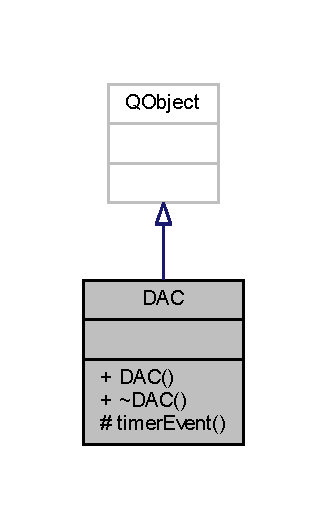
\includegraphics[width=157pt]{class_d_a_c__inherit__graph}
\end{center}
\end{figure}


D\+AC 的协作图\+:
\nopagebreak
\begin{figure}[H]
\begin{center}
\leavevmode
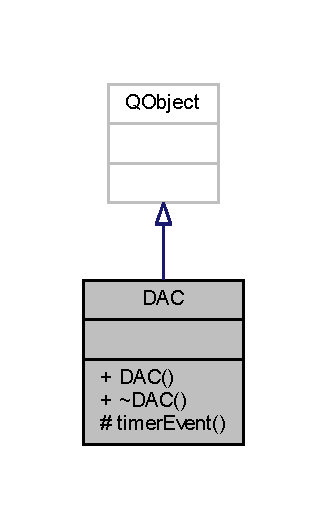
\includegraphics[width=157pt]{class_d_a_c__coll__graph}
\end{center}
\end{figure}
\subsection*{信号}
\begin{DoxyCompactItemize}
\item 
void \hyperlink{class_d_a_c_a3ba723a40a77bc08a713b5c83b1894db}{timeouted} (qint64)
\end{DoxyCompactItemize}
\subsection*{Public 成员函数}
\begin{DoxyCompactItemize}
\item 
\hyperlink{class_d_a_c_a5bc9520e1cdd8f4375fe939b08c2314f}{D\+AC} (H\+A\+N\+D\+LE $\ast$h, const \hyperlink{class_d_a_parameters}{D\+A\+Parameters} $\ast$para, int channel)
\item 
\hyperlink{class_d_a_c_a2a8f4f13338b7020e63c1ea04874e8a1}{$\sim$\+D\+AC} ()
\end{DoxyCompactItemize}
\subsection*{Protected 成员函数}
\begin{DoxyCompactItemize}
\item 
void \hyperlink{class_d_a_c_a5e12cba76ab2c580d531e3a84d18e180}{timer\+Event} (Q\+Timer\+Event $\ast$event)
\end{DoxyCompactItemize}


\subsection{构造及析构函数说明}
\index{D\+AC@{D\+AC}!D\+AC@{D\+AC}}
\index{D\+AC@{D\+AC}!D\+AC@{D\+AC}}
\subsubsection[{\texorpdfstring{D\+A\+C(\+H\+A\+N\+D\+L\+E $\ast$h, const D\+A\+Parameters $\ast$para, int channel)}{DAC(HANDLE *h, const DAParameters *para, int channel)}}]{\setlength{\rightskip}{0pt plus 5cm}D\+A\+C\+::\+D\+AC (
\begin{DoxyParamCaption}
\item[{H\+A\+N\+D\+LE $\ast$}]{h, }
\item[{const {\bf D\+A\+Parameters} $\ast$}]{para, }
\item[{int}]{channel}
\end{DoxyParamCaption}
)\hspace{0.3cm}{\ttfamily [explicit]}}\hypertarget{class_d_a_c_a5bc9520e1cdd8f4375fe939b08c2314f}{}\label{class_d_a_c_a5bc9520e1cdd8f4375fe939b08c2314f}
\index{D\+AC@{D\+AC}!````~D\+AC@{$\sim$\+D\+AC}}
\index{````~D\+AC@{$\sim$\+D\+AC}!D\+AC@{D\+AC}}
\subsubsection[{\texorpdfstring{$\sim$\+D\+A\+C()}{~DAC()}}]{\setlength{\rightskip}{0pt plus 5cm}D\+A\+C\+::$\sim$\+D\+AC (
\begin{DoxyParamCaption}
{}
\end{DoxyParamCaption}
)}\hypertarget{class_d_a_c_a2a8f4f13338b7020e63c1ea04874e8a1}{}\label{class_d_a_c_a2a8f4f13338b7020e63c1ea04874e8a1}


\subsection{成员函数说明}
\index{D\+AC@{D\+AC}!timeouted@{timeouted}}
\index{timeouted@{timeouted}!D\+AC@{D\+AC}}
\subsubsection[{\texorpdfstring{timeouted}{timeouted}}]{\setlength{\rightskip}{0pt plus 5cm}void D\+A\+C\+::timeouted (
\begin{DoxyParamCaption}
\item[{qint64}]{}
\end{DoxyParamCaption}
)\hspace{0.3cm}{\ttfamily [signal]}}\hypertarget{class_d_a_c_a3ba723a40a77bc08a713b5c83b1894db}{}\label{class_d_a_c_a3ba723a40a77bc08a713b5c83b1894db}
\index{D\+AC@{D\+AC}!timer\+Event@{timer\+Event}}
\index{timer\+Event@{timer\+Event}!D\+AC@{D\+AC}}
\subsubsection[{\texorpdfstring{timer\+Event(\+Q\+Timer\+Event $\ast$event)}{timerEvent(QTimerEvent *event)}}]{\setlength{\rightskip}{0pt plus 5cm}void D\+A\+C\+::timer\+Event (
\begin{DoxyParamCaption}
\item[{Q\+Timer\+Event $\ast$}]{event}
\end{DoxyParamCaption}
)\hspace{0.3cm}{\ttfamily [protected]}}\hypertarget{class_d_a_c_a5e12cba76ab2c580d531e3a84d18e180}{}\label{class_d_a_c_a5e12cba76ab2c580d531e3a84d18e180}


该类的文档由以下文件生成\+:\begin{DoxyCompactItemize}
\item 
\hyperlink{dac_8h}{dac.\+h}\item 
\hyperlink{dac_8cpp}{dac.\+cpp}\end{DoxyCompactItemize}

\hypertarget{class_d_a_parameters}{}\section{D\+A\+Parameters类 参考}
\label{class_d_a_parameters}\index{D\+A\+Parameters@{D\+A\+Parameters}}


{\ttfamily \#include $<$daparameters.\+h$>$}



类 D\+A\+Parameters 继承关系图\+:
\nopagebreak
\begin{figure}[H]
\begin{center}
\leavevmode
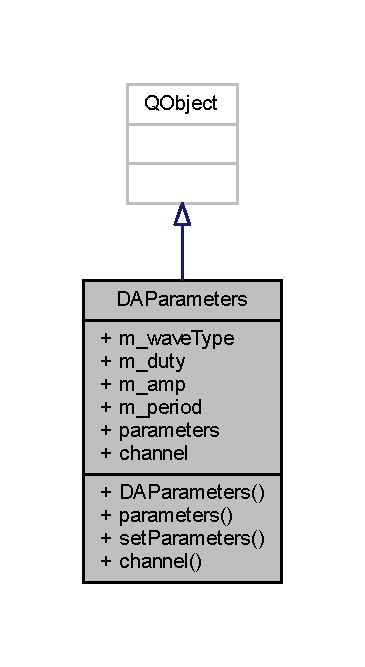
\includegraphics[width=175pt]{class_d_a_parameters__inherit__graph}
\end{center}
\end{figure}


D\+A\+Parameters 的协作图\+:
\nopagebreak
\begin{figure}[H]
\begin{center}
\leavevmode
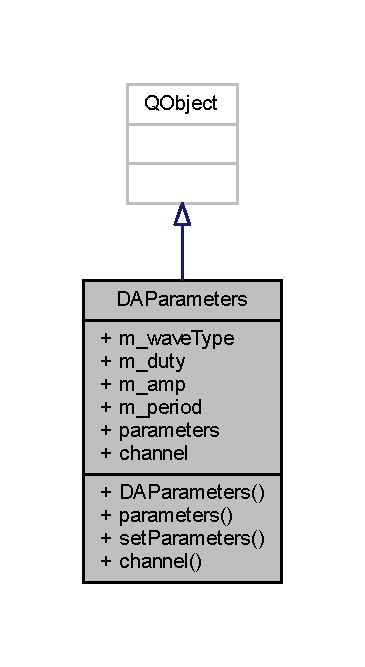
\includegraphics[width=175pt]{class_d_a_parameters__coll__graph}
\end{center}
\end{figure}
\subsection*{信号}
\begin{DoxyCompactItemize}
\item 
void \hyperlink{class_d_a_parameters_a81b97b0fc990adc38d4b94f022dedebb}{parameters\+Changed} ()
\item 
void \hyperlink{class_d_a_parameters_aecf569fb041e4e40fd4ab6665231f8b3}{channel\+Changed} ()
\end{DoxyCompactItemize}
\subsection*{Public 成员函数}
\begin{DoxyCompactItemize}
\item 
\hyperlink{class_d_a_parameters_acf3334279485abe4ad9ec96e2b714008}{D\+A\+Parameters} (Q\+Object $\ast$parent=0)
\item 
Q\+Variant\+List \hyperlink{class_d_a_parameters_a6f4b3462528b0eab3f4963957f649c1e}{parameters} ()
\item 
void \hyperlink{class_d_a_parameters_a5ddb50f4c96574fba8c8663c8e0a7ee7}{set\+Parameters} (Q\+Variant\+List list)
\item 
int \hyperlink{class_d_a_parameters_a69289518ead00f524fac5b8858268329}{channel} ()
\end{DoxyCompactItemize}
\subsection*{Public 属性}
\begin{DoxyCompactItemize}
\item 
int $\ast$ \hyperlink{class_d_a_parameters_a1228cc62d04f29283fc6739e4c70f5c6}{m\+\_\+wave\+Type}
\item 
int $\ast$ \hyperlink{class_d_a_parameters_a5294b0f7d5f7799a754e8cc24bbefb80}{m\+\_\+duty}
\item 
qreal $\ast$ \hyperlink{class_d_a_parameters_a56457c861795a1480baac2c25b739fab}{m\+\_\+amp}
\item 
int $\ast$ \hyperlink{class_d_a_parameters_abd4e4a7223eb42cd090f6dc7a991e4b8}{m\+\_\+period}
\end{DoxyCompactItemize}
\subsection*{属性}
\begin{DoxyCompactItemize}
\item 
Q\+Variant\+List \hyperlink{class_d_a_parameters_ab418da6f029448485c336c1cacdfacc7}{parameters}
\item 
int \hyperlink{class_d_a_parameters_a3eeae539e46310db5bc8ace9709b740e}{channel}
\end{DoxyCompactItemize}


\subsection{构造及析构函数说明}
\index{D\+A\+Parameters@{D\+A\+Parameters}!D\+A\+Parameters@{D\+A\+Parameters}}
\index{D\+A\+Parameters@{D\+A\+Parameters}!D\+A\+Parameters@{D\+A\+Parameters}}
\subsubsection[{\texorpdfstring{D\+A\+Parameters(\+Q\+Object $\ast$parent=0)}{DAParameters(QObject *parent=0)}}]{\setlength{\rightskip}{0pt plus 5cm}D\+A\+Parameters\+::\+D\+A\+Parameters (
\begin{DoxyParamCaption}
\item[{Q\+Object $\ast$}]{parent = {\ttfamily 0}}
\end{DoxyParamCaption}
)\hspace{0.3cm}{\ttfamily [explicit]}}\hypertarget{class_d_a_parameters_acf3334279485abe4ad9ec96e2b714008}{}\label{class_d_a_parameters_acf3334279485abe4ad9ec96e2b714008}


\subsection{成员函数说明}
\index{D\+A\+Parameters@{D\+A\+Parameters}!channel@{channel}}
\index{channel@{channel}!D\+A\+Parameters@{D\+A\+Parameters}}
\subsubsection[{\texorpdfstring{channel()}{channel()}}]{\setlength{\rightskip}{0pt plus 5cm}int D\+A\+Parameters\+::channel (
\begin{DoxyParamCaption}
{}
\end{DoxyParamCaption}
)}\hypertarget{class_d_a_parameters_a69289518ead00f524fac5b8858268329}{}\label{class_d_a_parameters_a69289518ead00f524fac5b8858268329}
\index{D\+A\+Parameters@{D\+A\+Parameters}!channel\+Changed@{channel\+Changed}}
\index{channel\+Changed@{channel\+Changed}!D\+A\+Parameters@{D\+A\+Parameters}}
\subsubsection[{\texorpdfstring{channel\+Changed}{channelChanged}}]{\setlength{\rightskip}{0pt plus 5cm}void D\+A\+Parameters\+::channel\+Changed (
\begin{DoxyParamCaption}
{}
\end{DoxyParamCaption}
)\hspace{0.3cm}{\ttfamily [signal]}}\hypertarget{class_d_a_parameters_aecf569fb041e4e40fd4ab6665231f8b3}{}\label{class_d_a_parameters_aecf569fb041e4e40fd4ab6665231f8b3}
\index{D\+A\+Parameters@{D\+A\+Parameters}!parameters@{parameters}}
\index{parameters@{parameters}!D\+A\+Parameters@{D\+A\+Parameters}}
\subsubsection[{\texorpdfstring{parameters()}{parameters()}}]{\setlength{\rightskip}{0pt plus 5cm}Q\+Variant\+List D\+A\+Parameters\+::parameters (
\begin{DoxyParamCaption}
{}
\end{DoxyParamCaption}
)}\hypertarget{class_d_a_parameters_a6f4b3462528b0eab3f4963957f649c1e}{}\label{class_d_a_parameters_a6f4b3462528b0eab3f4963957f649c1e}
\index{D\+A\+Parameters@{D\+A\+Parameters}!parameters\+Changed@{parameters\+Changed}}
\index{parameters\+Changed@{parameters\+Changed}!D\+A\+Parameters@{D\+A\+Parameters}}
\subsubsection[{\texorpdfstring{parameters\+Changed}{parametersChanged}}]{\setlength{\rightskip}{0pt plus 5cm}void D\+A\+Parameters\+::parameters\+Changed (
\begin{DoxyParamCaption}
{}
\end{DoxyParamCaption}
)\hspace{0.3cm}{\ttfamily [signal]}}\hypertarget{class_d_a_parameters_a81b97b0fc990adc38d4b94f022dedebb}{}\label{class_d_a_parameters_a81b97b0fc990adc38d4b94f022dedebb}
\index{D\+A\+Parameters@{D\+A\+Parameters}!set\+Parameters@{set\+Parameters}}
\index{set\+Parameters@{set\+Parameters}!D\+A\+Parameters@{D\+A\+Parameters}}
\subsubsection[{\texorpdfstring{set\+Parameters(\+Q\+Variant\+List list)}{setParameters(QVariantList list)}}]{\setlength{\rightskip}{0pt plus 5cm}void D\+A\+Parameters\+::set\+Parameters (
\begin{DoxyParamCaption}
\item[{Q\+Variant\+List}]{list}
\end{DoxyParamCaption}
)}\hypertarget{class_d_a_parameters_a5ddb50f4c96574fba8c8663c8e0a7ee7}{}\label{class_d_a_parameters_a5ddb50f4c96574fba8c8663c8e0a7ee7}


\subsection{类成员变量说明}
\index{D\+A\+Parameters@{D\+A\+Parameters}!m\+\_\+amp@{m\+\_\+amp}}
\index{m\+\_\+amp@{m\+\_\+amp}!D\+A\+Parameters@{D\+A\+Parameters}}
\subsubsection[{\texorpdfstring{m\+\_\+amp}{m_amp}}]{\setlength{\rightskip}{0pt plus 5cm}qreal$\ast$ D\+A\+Parameters\+::m\+\_\+amp}\hypertarget{class_d_a_parameters_a56457c861795a1480baac2c25b739fab}{}\label{class_d_a_parameters_a56457c861795a1480baac2c25b739fab}
\index{D\+A\+Parameters@{D\+A\+Parameters}!m\+\_\+duty@{m\+\_\+duty}}
\index{m\+\_\+duty@{m\+\_\+duty}!D\+A\+Parameters@{D\+A\+Parameters}}
\subsubsection[{\texorpdfstring{m\+\_\+duty}{m_duty}}]{\setlength{\rightskip}{0pt plus 5cm}int$\ast$ D\+A\+Parameters\+::m\+\_\+duty}\hypertarget{class_d_a_parameters_a5294b0f7d5f7799a754e8cc24bbefb80}{}\label{class_d_a_parameters_a5294b0f7d5f7799a754e8cc24bbefb80}
\index{D\+A\+Parameters@{D\+A\+Parameters}!m\+\_\+period@{m\+\_\+period}}
\index{m\+\_\+period@{m\+\_\+period}!D\+A\+Parameters@{D\+A\+Parameters}}
\subsubsection[{\texorpdfstring{m\+\_\+period}{m_period}}]{\setlength{\rightskip}{0pt plus 5cm}int$\ast$ D\+A\+Parameters\+::m\+\_\+period}\hypertarget{class_d_a_parameters_abd4e4a7223eb42cd090f6dc7a991e4b8}{}\label{class_d_a_parameters_abd4e4a7223eb42cd090f6dc7a991e4b8}
\index{D\+A\+Parameters@{D\+A\+Parameters}!m\+\_\+wave\+Type@{m\+\_\+wave\+Type}}
\index{m\+\_\+wave\+Type@{m\+\_\+wave\+Type}!D\+A\+Parameters@{D\+A\+Parameters}}
\subsubsection[{\texorpdfstring{m\+\_\+wave\+Type}{m_waveType}}]{\setlength{\rightskip}{0pt plus 5cm}int$\ast$ D\+A\+Parameters\+::m\+\_\+wave\+Type}\hypertarget{class_d_a_parameters_a1228cc62d04f29283fc6739e4c70f5c6}{}\label{class_d_a_parameters_a1228cc62d04f29283fc6739e4c70f5c6}


\subsection{属性说明}
\index{D\+A\+Parameters@{D\+A\+Parameters}!channel@{channel}}
\index{channel@{channel}!D\+A\+Parameters@{D\+A\+Parameters}}
\subsubsection[{\texorpdfstring{channel}{channel}}]{\setlength{\rightskip}{0pt plus 5cm}int D\+A\+Parameters\+::channel\hspace{0.3cm}{\ttfamily [read]}}\hypertarget{class_d_a_parameters_a3eeae539e46310db5bc8ace9709b740e}{}\label{class_d_a_parameters_a3eeae539e46310db5bc8ace9709b740e}
\index{D\+A\+Parameters@{D\+A\+Parameters}!parameters@{parameters}}
\index{parameters@{parameters}!D\+A\+Parameters@{D\+A\+Parameters}}
\subsubsection[{\texorpdfstring{parameters}{parameters}}]{\setlength{\rightskip}{0pt plus 5cm}Q\+Variant\+List D\+A\+Parameters\+::parameters\hspace{0.3cm}{\ttfamily [read]}, {\ttfamily [write]}}\hypertarget{class_d_a_parameters_ab418da6f029448485c336c1cacdfacc7}{}\label{class_d_a_parameters_ab418da6f029448485c336c1cacdfacc7}


该类的文档由以下文件生成\+:\begin{DoxyCompactItemize}
\item 
\hyperlink{daparameters_8h}{daparameters.\+h}\item 
\hyperlink{daparameters_8cpp}{daparameters.\+cpp}\end{DoxyCompactItemize}

\hypertarget{class_d_a_q}{}\section{D\+A\+Q类 参考}
\label{class_d_a_q}\index{D\+AQ@{D\+AQ}}


{\ttfamily \#include $<$daq.\+h$>$}



类 D\+AQ 继承关系图\+:
\nopagebreak
\begin{figure}[H]
\begin{center}
\leavevmode
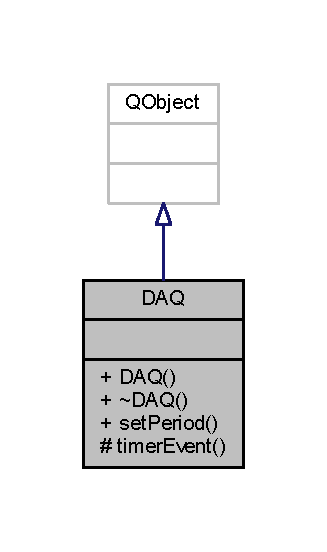
\includegraphics[width=157pt]{class_d_a_q__inherit__graph}
\end{center}
\end{figure}


D\+AQ 的协作图\+:
\nopagebreak
\begin{figure}[H]
\begin{center}
\leavevmode
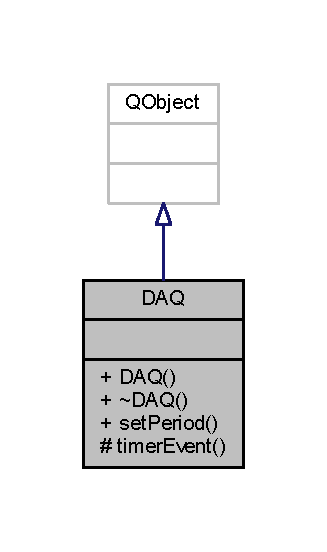
\includegraphics[width=157pt]{class_d_a_q__coll__graph}
\end{center}
\end{figure}
\subsection*{Public 槽}
\begin{DoxyCompactItemize}
\item 
void \hyperlink{class_d_a_q_ad42b0d02d4af3fb7464eb900e2f0dc58}{set\+Period} (int p)
\end{DoxyCompactItemize}
\subsection*{信号}
\begin{DoxyCompactItemize}
\item 
void \hyperlink{class_d_a_q_ace1e99bc4fd8976a9aec05a6cf70b22b}{acquired} (const Q\+Date\+Time \&)
\end{DoxyCompactItemize}
\subsection*{Public 成员函数}
\begin{DoxyCompactItemize}
\item 
\hyperlink{class_d_a_q_abbe9423ce4f1699ec10335079432cb2f}{D\+AQ} (H\+A\+N\+D\+LE $\ast$handle, qint16 $\ast$buffer)
\item 
\hyperlink{class_d_a_q_ab4e9db33b2aec273f9aca5493af60870}{$\sim$\+D\+AQ} ()
\end{DoxyCompactItemize}
\subsection*{Protected 成员函数}
\begin{DoxyCompactItemize}
\item 
void \hyperlink{class_d_a_q_a6671442402cd7209dfb8fedb7265a098}{timer\+Event} (Q\+Timer\+Event $\ast$event)
\end{DoxyCompactItemize}


\subsection{构造及析构函数说明}
\index{D\+AQ@{D\+AQ}!D\+AQ@{D\+AQ}}
\index{D\+AQ@{D\+AQ}!D\+AQ@{D\+AQ}}
\subsubsection[{\texorpdfstring{D\+A\+Q(\+H\+A\+N\+D\+L\+E $\ast$handle, qint16 $\ast$buffer)}{DAQ(HANDLE *handle, qint16 *buffer)}}]{\setlength{\rightskip}{0pt plus 5cm}D\+A\+Q\+::\+D\+AQ (
\begin{DoxyParamCaption}
\item[{H\+A\+N\+D\+LE $\ast$}]{handle, }
\item[{qint16 $\ast$}]{buffer}
\end{DoxyParamCaption}
)\hspace{0.3cm}{\ttfamily [explicit]}}\hypertarget{class_d_a_q_abbe9423ce4f1699ec10335079432cb2f}{}\label{class_d_a_q_abbe9423ce4f1699ec10335079432cb2f}
\index{D\+AQ@{D\+AQ}!````~D\+AQ@{$\sim$\+D\+AQ}}
\index{````~D\+AQ@{$\sim$\+D\+AQ}!D\+AQ@{D\+AQ}}
\subsubsection[{\texorpdfstring{$\sim$\+D\+A\+Q()}{~DAQ()}}]{\setlength{\rightskip}{0pt plus 5cm}D\+A\+Q\+::$\sim$\+D\+AQ (
\begin{DoxyParamCaption}
{}
\end{DoxyParamCaption}
)}\hypertarget{class_d_a_q_ab4e9db33b2aec273f9aca5493af60870}{}\label{class_d_a_q_ab4e9db33b2aec273f9aca5493af60870}


\subsection{成员函数说明}
\index{D\+AQ@{D\+AQ}!acquired@{acquired}}
\index{acquired@{acquired}!D\+AQ@{D\+AQ}}
\subsubsection[{\texorpdfstring{acquired}{acquired}}]{\setlength{\rightskip}{0pt plus 5cm}void D\+A\+Q\+::acquired (
\begin{DoxyParamCaption}
\item[{const Q\+Date\+Time \&}]{}
\end{DoxyParamCaption}
)\hspace{0.3cm}{\ttfamily [signal]}}\hypertarget{class_d_a_q_ace1e99bc4fd8976a9aec05a6cf70b22b}{}\label{class_d_a_q_ace1e99bc4fd8976a9aec05a6cf70b22b}
\index{D\+AQ@{D\+AQ}!set\+Period@{set\+Period}}
\index{set\+Period@{set\+Period}!D\+AQ@{D\+AQ}}
\subsubsection[{\texorpdfstring{set\+Period}{setPeriod}}]{\setlength{\rightskip}{0pt plus 5cm}void D\+A\+Q\+::set\+Period (
\begin{DoxyParamCaption}
\item[{int}]{p}
\end{DoxyParamCaption}
)\hspace{0.3cm}{\ttfamily [slot]}}\hypertarget{class_d_a_q_ad42b0d02d4af3fb7464eb900e2f0dc58}{}\label{class_d_a_q_ad42b0d02d4af3fb7464eb900e2f0dc58}
\index{D\+AQ@{D\+AQ}!timer\+Event@{timer\+Event}}
\index{timer\+Event@{timer\+Event}!D\+AQ@{D\+AQ}}
\subsubsection[{\texorpdfstring{timer\+Event(\+Q\+Timer\+Event $\ast$event)}{timerEvent(QTimerEvent *event)}}]{\setlength{\rightskip}{0pt plus 5cm}void D\+A\+Q\+::timer\+Event (
\begin{DoxyParamCaption}
\item[{Q\+Timer\+Event $\ast$}]{event}
\end{DoxyParamCaption}
)\hspace{0.3cm}{\ttfamily [protected]}}\hypertarget{class_d_a_q_a6671442402cd7209dfb8fedb7265a098}{}\label{class_d_a_q_a6671442402cd7209dfb8fedb7265a098}


该类的文档由以下文件生成\+:\begin{DoxyCompactItemize}
\item 
\hyperlink{daq_8h}{daq.\+h}\item 
\hyperlink{daq_8cpp}{daq.\+cpp}\end{DoxyCompactItemize}

\hypertarget{class_database}{}\section{Database类 参考}
\label{class_database}\index{Database@{Database}}


{\ttfamily \#include $<$database.\+h$>$}



类 Database 继承关系图\+:
\nopagebreak
\begin{figure}[H]
\begin{center}
\leavevmode
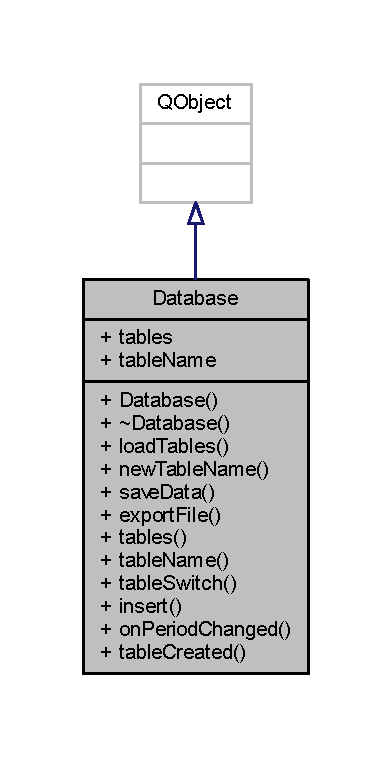
\includegraphics[width=188pt]{class_database__inherit__graph}
\end{center}
\end{figure}


Database 的协作图\+:
\nopagebreak
\begin{figure}[H]
\begin{center}
\leavevmode
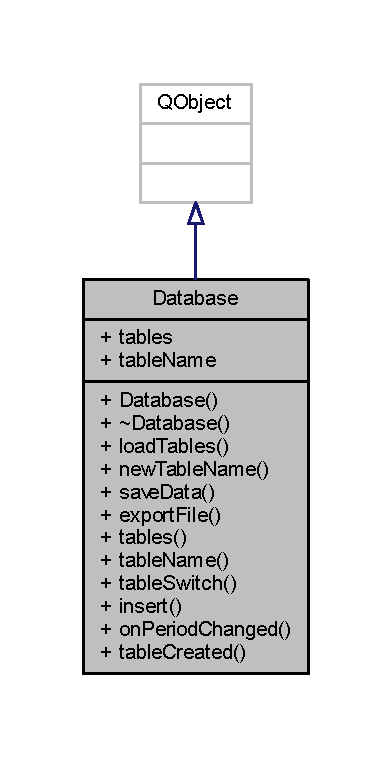
\includegraphics[width=188pt]{class_database__coll__graph}
\end{center}
\end{figure}
\subsection*{Public 槽}
\begin{DoxyCompactItemize}
\item 
void \hyperlink{class_database_a5cafa53304f3ff79a2487f5333cab8ad}{table\+Switch} (bool s)
\item 
void \hyperlink{class_database_a2262e223186a88b1ac0f88245bfaab71}{insert} (const Q\+Date\+Time \&datetime)
\item 
void \hyperlink{class_database_a857e6024cbfab56a3f3521ccc6769cf4}{on\+Period\+Changed} (int p)
\item 
void \hyperlink{class_database_af6cffa238311bf9d398f401c314160bf}{table\+Created} ()
\end{DoxyCompactItemize}
\subsection*{信号}
\begin{DoxyCompactItemize}
\item 
void \hyperlink{class_database_aa804ee053ba71d1e7c711a440968b9bc}{tables\+Changed} ()
\item 
void \hyperlink{class_database_a0ed84bd7f656e5fabadd579a0cbcbc57}{table\+Name\+Changed} ()
\item 
void \hyperlink{class_database_a1581c3afe4b3b9427620a55f29e0910b}{export\+X\+L\+SX} (const Q\+String \&, const Q\+String \&)
\item 
void \hyperlink{class_database_a083b4f32eff1dd87f48f6ccb46f3218e}{data\+Insert} (const Q\+Date\+Time \&, const Q\+String \&)
\item 
void \hyperlink{class_database_a4534ad8a6b59a7bf06d287911c38421a}{create\+Table} (const Q\+String \&)
\end{DoxyCompactItemize}
\subsection*{Public 成员函数}
\begin{DoxyCompactItemize}
\item 
\hyperlink{class_database_acad5a1c9dd5a5051e3967024dc96373a}{Database} (qint16 $\ast$buffer)
\item 
\hyperlink{class_database_a84d399a2ad58d69daab9b05330e1316d}{$\sim$\+Database} ()
\item 
Q\+\_\+\+I\+N\+V\+O\+K\+A\+B\+LE void \hyperlink{class_database_a8eecdb8ab49878d43a41d5e29c3c35a2}{load\+Tables} ()
\item 
Q\+\_\+\+I\+N\+V\+O\+K\+A\+B\+LE Q\+String \hyperlink{class_database_a2c471d41d2dd4341ff510e06a0c8c6a5}{new\+Table\+Name} ()
\item 
Q\+\_\+\+I\+N\+V\+O\+K\+A\+B\+LE void \hyperlink{class_database_a6192c09a9cba8435c61c779d519e57b0}{save\+Data} (bool s)
\item 
Q\+\_\+\+I\+N\+V\+O\+K\+A\+B\+LE void \hyperlink{class_database_adcec92191ed1c8773bcf82f676a0e87b}{export\+File} (const Q\+String \&\hyperlink{class_database_a9f617c90d57d4c5b14e96e51c1aea92b}{table\+Name}, const Q\+String \&suffix)
\item 
Q\+Variant \hyperlink{class_database_a47600e88e0ff9dea23b9e3ee27ed55bf}{tables} ()
\item 
Q\+String \hyperlink{class_database_aa5f9ba4502bd54b08a1c04381cc8d361}{table\+Name} ()
\end{DoxyCompactItemize}
\subsection*{属性}
\begin{DoxyCompactItemize}
\item 
Q\+Variant \hyperlink{class_database_ad44cff8b67b203182ef6d2b8f01126cf}{tables}
\item 
Q\+String \hyperlink{class_database_a9f617c90d57d4c5b14e96e51c1aea92b}{table\+Name}
\end{DoxyCompactItemize}


\subsection{构造及析构函数说明}
\index{Database@{Database}!Database@{Database}}
\index{Database@{Database}!Database@{Database}}
\subsubsection[{\texorpdfstring{Database(qint16 $\ast$buffer)}{Database(qint16 *buffer)}}]{\setlength{\rightskip}{0pt plus 5cm}Database\+::\+Database (
\begin{DoxyParamCaption}
\item[{qint16 $\ast$}]{buffer}
\end{DoxyParamCaption}
)\hspace{0.3cm}{\ttfamily [explicit]}}\hypertarget{class_database_acad5a1c9dd5a5051e3967024dc96373a}{}\label{class_database_acad5a1c9dd5a5051e3967024dc96373a}
\index{Database@{Database}!````~Database@{$\sim$\+Database}}
\index{````~Database@{$\sim$\+Database}!Database@{Database}}
\subsubsection[{\texorpdfstring{$\sim$\+Database()}{~Database()}}]{\setlength{\rightskip}{0pt plus 5cm}Database\+::$\sim$\+Database (
\begin{DoxyParamCaption}
{}
\end{DoxyParamCaption}
)}\hypertarget{class_database_a84d399a2ad58d69daab9b05330e1316d}{}\label{class_database_a84d399a2ad58d69daab9b05330e1316d}


\subsection{成员函数说明}
\index{Database@{Database}!create\+Table@{create\+Table}}
\index{create\+Table@{create\+Table}!Database@{Database}}
\subsubsection[{\texorpdfstring{create\+Table}{createTable}}]{\setlength{\rightskip}{0pt plus 5cm}void Database\+::create\+Table (
\begin{DoxyParamCaption}
\item[{const Q\+String \&}]{}
\end{DoxyParamCaption}
)\hspace{0.3cm}{\ttfamily [signal]}}\hypertarget{class_database_a4534ad8a6b59a7bf06d287911c38421a}{}\label{class_database_a4534ad8a6b59a7bf06d287911c38421a}
\index{Database@{Database}!data\+Insert@{data\+Insert}}
\index{data\+Insert@{data\+Insert}!Database@{Database}}
\subsubsection[{\texorpdfstring{data\+Insert}{dataInsert}}]{\setlength{\rightskip}{0pt plus 5cm}void Database\+::data\+Insert (
\begin{DoxyParamCaption}
\item[{const Q\+Date\+Time \&}]{, }
\item[{const Q\+String \&}]{}
\end{DoxyParamCaption}
)\hspace{0.3cm}{\ttfamily [signal]}}\hypertarget{class_database_a083b4f32eff1dd87f48f6ccb46f3218e}{}\label{class_database_a083b4f32eff1dd87f48f6ccb46f3218e}
\index{Database@{Database}!export\+File@{export\+File}}
\index{export\+File@{export\+File}!Database@{Database}}
\subsubsection[{\texorpdfstring{export\+File(const Q\+String \&table\+Name, const Q\+String \&suffix)}{exportFile(const QString &tableName, const QString &suffix)}}]{\setlength{\rightskip}{0pt plus 5cm}void Database\+::export\+File (
\begin{DoxyParamCaption}
\item[{const Q\+String \&}]{table\+Name, }
\item[{const Q\+String \&}]{suffix}
\end{DoxyParamCaption}
)}\hypertarget{class_database_adcec92191ed1c8773bcf82f676a0e87b}{}\label{class_database_adcec92191ed1c8773bcf82f676a0e87b}
\index{Database@{Database}!export\+X\+L\+SX@{export\+X\+L\+SX}}
\index{export\+X\+L\+SX@{export\+X\+L\+SX}!Database@{Database}}
\subsubsection[{\texorpdfstring{export\+X\+L\+SX}{exportXLSX}}]{\setlength{\rightskip}{0pt plus 5cm}void Database\+::export\+X\+L\+SX (
\begin{DoxyParamCaption}
\item[{const Q\+String \&}]{, }
\item[{const Q\+String \&}]{}
\end{DoxyParamCaption}
)\hspace{0.3cm}{\ttfamily [signal]}}\hypertarget{class_database_a1581c3afe4b3b9427620a55f29e0910b}{}\label{class_database_a1581c3afe4b3b9427620a55f29e0910b}
\index{Database@{Database}!insert@{insert}}
\index{insert@{insert}!Database@{Database}}
\subsubsection[{\texorpdfstring{insert}{insert}}]{\setlength{\rightskip}{0pt plus 5cm}void Database\+::insert (
\begin{DoxyParamCaption}
\item[{const Q\+Date\+Time \&}]{datetime}
\end{DoxyParamCaption}
)\hspace{0.3cm}{\ttfamily [slot]}}\hypertarget{class_database_a2262e223186a88b1ac0f88245bfaab71}{}\label{class_database_a2262e223186a88b1ac0f88245bfaab71}
\index{Database@{Database}!load\+Tables@{load\+Tables}}
\index{load\+Tables@{load\+Tables}!Database@{Database}}
\subsubsection[{\texorpdfstring{load\+Tables()}{loadTables()}}]{\setlength{\rightskip}{0pt plus 5cm}void Database\+::load\+Tables (
\begin{DoxyParamCaption}
{}
\end{DoxyParamCaption}
)}\hypertarget{class_database_a8eecdb8ab49878d43a41d5e29c3c35a2}{}\label{class_database_a8eecdb8ab49878d43a41d5e29c3c35a2}
\index{Database@{Database}!new\+Table\+Name@{new\+Table\+Name}}
\index{new\+Table\+Name@{new\+Table\+Name}!Database@{Database}}
\subsubsection[{\texorpdfstring{new\+Table\+Name()}{newTableName()}}]{\setlength{\rightskip}{0pt plus 5cm}Q\+String Database\+::new\+Table\+Name (
\begin{DoxyParamCaption}
{}
\end{DoxyParamCaption}
)}\hypertarget{class_database_a2c471d41d2dd4341ff510e06a0c8c6a5}{}\label{class_database_a2c471d41d2dd4341ff510e06a0c8c6a5}
\index{Database@{Database}!on\+Period\+Changed@{on\+Period\+Changed}}
\index{on\+Period\+Changed@{on\+Period\+Changed}!Database@{Database}}
\subsubsection[{\texorpdfstring{on\+Period\+Changed}{onPeriodChanged}}]{\setlength{\rightskip}{0pt plus 5cm}void Database\+::on\+Period\+Changed (
\begin{DoxyParamCaption}
\item[{int}]{p}
\end{DoxyParamCaption}
)\hspace{0.3cm}{\ttfamily [slot]}}\hypertarget{class_database_a857e6024cbfab56a3f3521ccc6769cf4}{}\label{class_database_a857e6024cbfab56a3f3521ccc6769cf4}
\index{Database@{Database}!save\+Data@{save\+Data}}
\index{save\+Data@{save\+Data}!Database@{Database}}
\subsubsection[{\texorpdfstring{save\+Data(bool s)}{saveData(bool s)}}]{\setlength{\rightskip}{0pt plus 5cm}void Database\+::save\+Data (
\begin{DoxyParamCaption}
\item[{bool}]{s}
\end{DoxyParamCaption}
)}\hypertarget{class_database_a6192c09a9cba8435c61c779d519e57b0}{}\label{class_database_a6192c09a9cba8435c61c779d519e57b0}
\index{Database@{Database}!table\+Created@{table\+Created}}
\index{table\+Created@{table\+Created}!Database@{Database}}
\subsubsection[{\texorpdfstring{table\+Created}{tableCreated}}]{\setlength{\rightskip}{0pt plus 5cm}void Database\+::table\+Created (
\begin{DoxyParamCaption}
{}
\end{DoxyParamCaption}
)\hspace{0.3cm}{\ttfamily [slot]}}\hypertarget{class_database_af6cffa238311bf9d398f401c314160bf}{}\label{class_database_af6cffa238311bf9d398f401c314160bf}
\index{Database@{Database}!table\+Name@{table\+Name}}
\index{table\+Name@{table\+Name}!Database@{Database}}
\subsubsection[{\texorpdfstring{table\+Name()}{tableName()}}]{\setlength{\rightskip}{0pt plus 5cm}Q\+String Database\+::table\+Name (
\begin{DoxyParamCaption}
{}
\end{DoxyParamCaption}
)}\hypertarget{class_database_aa5f9ba4502bd54b08a1c04381cc8d361}{}\label{class_database_aa5f9ba4502bd54b08a1c04381cc8d361}
\index{Database@{Database}!table\+Name\+Changed@{table\+Name\+Changed}}
\index{table\+Name\+Changed@{table\+Name\+Changed}!Database@{Database}}
\subsubsection[{\texorpdfstring{table\+Name\+Changed}{tableNameChanged}}]{\setlength{\rightskip}{0pt plus 5cm}void Database\+::table\+Name\+Changed (
\begin{DoxyParamCaption}
{}
\end{DoxyParamCaption}
)\hspace{0.3cm}{\ttfamily [signal]}}\hypertarget{class_database_a0ed84bd7f656e5fabadd579a0cbcbc57}{}\label{class_database_a0ed84bd7f656e5fabadd579a0cbcbc57}
\index{Database@{Database}!tables@{tables}}
\index{tables@{tables}!Database@{Database}}
\subsubsection[{\texorpdfstring{tables()}{tables()}}]{\setlength{\rightskip}{0pt plus 5cm}Q\+Variant Database\+::tables (
\begin{DoxyParamCaption}
{}
\end{DoxyParamCaption}
)}\hypertarget{class_database_a47600e88e0ff9dea23b9e3ee27ed55bf}{}\label{class_database_a47600e88e0ff9dea23b9e3ee27ed55bf}
\index{Database@{Database}!tables\+Changed@{tables\+Changed}}
\index{tables\+Changed@{tables\+Changed}!Database@{Database}}
\subsubsection[{\texorpdfstring{tables\+Changed}{tablesChanged}}]{\setlength{\rightskip}{0pt plus 5cm}void Database\+::tables\+Changed (
\begin{DoxyParamCaption}
{}
\end{DoxyParamCaption}
)\hspace{0.3cm}{\ttfamily [signal]}}\hypertarget{class_database_aa804ee053ba71d1e7c711a440968b9bc}{}\label{class_database_aa804ee053ba71d1e7c711a440968b9bc}
\index{Database@{Database}!table\+Switch@{table\+Switch}}
\index{table\+Switch@{table\+Switch}!Database@{Database}}
\subsubsection[{\texorpdfstring{table\+Switch}{tableSwitch}}]{\setlength{\rightskip}{0pt plus 5cm}void Database\+::table\+Switch (
\begin{DoxyParamCaption}
\item[{bool}]{s}
\end{DoxyParamCaption}
)\hspace{0.3cm}{\ttfamily [slot]}}\hypertarget{class_database_a5cafa53304f3ff79a2487f5333cab8ad}{}\label{class_database_a5cafa53304f3ff79a2487f5333cab8ad}


\subsection{属性说明}
\index{Database@{Database}!table\+Name@{table\+Name}}
\index{table\+Name@{table\+Name}!Database@{Database}}
\subsubsection[{\texorpdfstring{table\+Name}{tableName}}]{\setlength{\rightskip}{0pt plus 5cm}Q\+String Database\+::table\+Name\hspace{0.3cm}{\ttfamily [read]}}\hypertarget{class_database_a9f617c90d57d4c5b14e96e51c1aea92b}{}\label{class_database_a9f617c90d57d4c5b14e96e51c1aea92b}
\index{Database@{Database}!tables@{tables}}
\index{tables@{tables}!Database@{Database}}
\subsubsection[{\texorpdfstring{tables}{tables}}]{\setlength{\rightskip}{0pt plus 5cm}Q\+Variant Database\+::tables\hspace{0.3cm}{\ttfamily [read]}}\hypertarget{class_database_ad44cff8b67b203182ef6d2b8f01126cf}{}\label{class_database_ad44cff8b67b203182ef6d2b8f01126cf}


该类的文档由以下文件生成\+:\begin{DoxyCompactItemize}
\item 
\hyperlink{database_8h}{database.\+h}\item 
\hyperlink{database_8cpp}{database.\+cpp}\end{DoxyCompactItemize}

\hypertarget{class_data_source}{}\section{Data\+Source类 参考}
\label{class_data_source}\index{Data\+Source@{Data\+Source}}


{\ttfamily \#include $<$datasource.\+h$>$}



类 Data\+Source 继承关系图\+:
\nopagebreak
\begin{figure}[H]
\begin{center}
\leavevmode
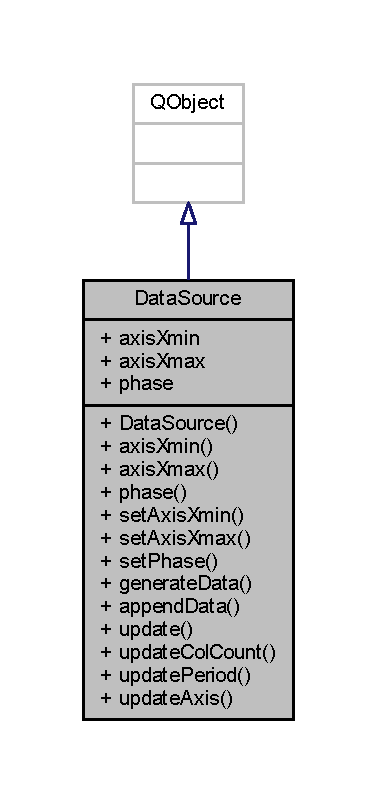
\includegraphics[width=181pt]{class_data_source__inherit__graph}
\end{center}
\end{figure}


Data\+Source 的协作图\+:
\nopagebreak
\begin{figure}[H]
\begin{center}
\leavevmode
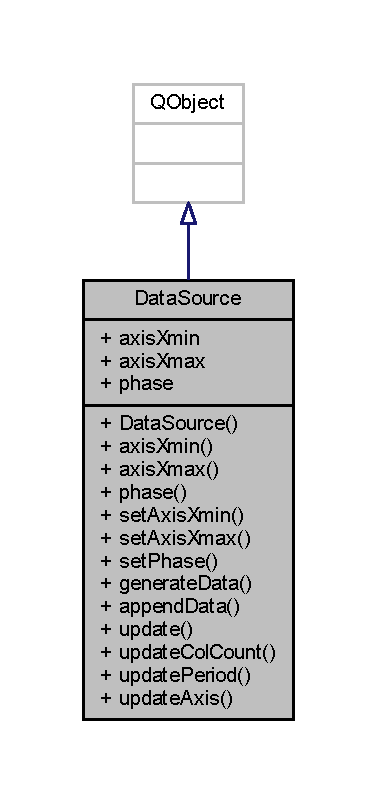
\includegraphics[width=181pt]{class_data_source__coll__graph}
\end{center}
\end{figure}
\subsection*{Public 槽}
\begin{DoxyCompactItemize}
\item 
void \hyperlink{class_data_source_a497de454187a552636ad55a019f954b6}{generate\+Data} (int row\+Count, int col\+Count)
\item 
void \hyperlink{class_data_source_a441d29c53c284cbe24e66054e5ea2d5f}{append\+Data} ()
\item 
void \hyperlink{class_data_source_a062d2e31fd30def382a9ecd7bdf96f67}{update} (int index, Q\+Abstract\+Series $\ast$series)
\item 
void \hyperlink{class_data_source_a1dc22689c55dd2f548573048b139e1cc}{update\+Col\+Count} (uint col)
\item 
void \hyperlink{class_data_source_aee37693c57b35d37e12cca66f7fae7cd}{update\+Period} (int p)
\item 
void \hyperlink{class_data_source_a639b431dd2114b68e2f3fcca08e549c2}{update\+Axis} ()
\end{DoxyCompactItemize}
\subsection*{信号}
\begin{DoxyCompactItemize}
\item 
void \hyperlink{class_data_source_a4e26914c46eb97ee3de4fec03cbb54e6}{axis\+Xmin\+Changed} ()
\item 
void \hyperlink{class_data_source_a709fe7d94ba3d2a86b487c132b295f8e}{axis\+Xmax\+Changed} ()
\item 
void \hyperlink{class_data_source_abd9b360e415e2e95e41837454d35443e}{phase\+Changed} ()
\end{DoxyCompactItemize}
\subsection*{Public 成员函数}
\begin{DoxyCompactItemize}
\item 
\hyperlink{class_data_source_adc0eb0527c0c7ea3fa924116078a9564}{Data\+Source} (qint16 $\ast$buffer, \hyperlink{class_timer}{Timer} $\ast$timer, Q\+Object $\ast$parent)
\item 
qreal \hyperlink{class_data_source_afe91344f3c61bab470d6daf522d9f0b9}{axis\+Xmin} ()
\item 
qreal \hyperlink{class_data_source_a6e3609869fd0f781ff7b3f8b0a8bcc63}{axis\+Xmax} ()
\item 
qreal \hyperlink{class_data_source_a2059193093f18defeabcd360d815a47a}{phase} ()
\item 
void \hyperlink{class_data_source_a0757ea4dea841dc0b9586d0830dcbb84}{set\+Axis\+Xmin} (qreal x)
\item 
void \hyperlink{class_data_source_a1d874305fb6c97fa1dc8174c51898c14}{set\+Axis\+Xmax} (qreal x)
\item 
void \hyperlink{class_data_source_af8bbe6caa786e6721da8e1ee570381de}{set\+Phase} (qreal x)
\end{DoxyCompactItemize}
\subsection*{属性}
\begin{DoxyCompactItemize}
\item 
qreal \hyperlink{class_data_source_a8222c7e324caaa4d802d6af493f7c53c}{axis\+Xmin}
\item 
qreal \hyperlink{class_data_source_ac03049a5aedd86f7f660c07d37541109}{axis\+Xmax}
\item 
qreal \hyperlink{class_data_source_a3e863a4ef50683165d94f418b3567486}{phase}
\end{DoxyCompactItemize}


\subsection{构造及析构函数说明}
\index{Data\+Source@{Data\+Source}!Data\+Source@{Data\+Source}}
\index{Data\+Source@{Data\+Source}!Data\+Source@{Data\+Source}}
\subsubsection[{\texorpdfstring{Data\+Source(qint16 $\ast$buffer, Timer $\ast$timer, Q\+Object $\ast$parent)}{DataSource(qint16 *buffer, Timer *timer, QObject *parent)}}]{\setlength{\rightskip}{0pt plus 5cm}Q\+T\+\_\+\+C\+H\+A\+R\+T\+S\+\_\+\+U\+S\+E\+\_\+\+N\+A\+M\+E\+S\+P\+A\+CE Data\+Source\+::\+Data\+Source (
\begin{DoxyParamCaption}
\item[{qint16 $\ast$}]{buffer, }
\item[{{\bf Timer} $\ast$}]{timer, }
\item[{Q\+Object $\ast$}]{parent}
\end{DoxyParamCaption}
)\hspace{0.3cm}{\ttfamily [explicit]}}\hypertarget{class_data_source_adc0eb0527c0c7ea3fa924116078a9564}{}\label{class_data_source_adc0eb0527c0c7ea3fa924116078a9564}


\subsection{成员函数说明}
\index{Data\+Source@{Data\+Source}!append\+Data@{append\+Data}}
\index{append\+Data@{append\+Data}!Data\+Source@{Data\+Source}}
\subsubsection[{\texorpdfstring{append\+Data}{appendData}}]{\setlength{\rightskip}{0pt plus 5cm}void Data\+Source\+::append\+Data (
\begin{DoxyParamCaption}
{}
\end{DoxyParamCaption}
)\hspace{0.3cm}{\ttfamily [slot]}}\hypertarget{class_data_source_a441d29c53c284cbe24e66054e5ea2d5f}{}\label{class_data_source_a441d29c53c284cbe24e66054e5ea2d5f}
\index{Data\+Source@{Data\+Source}!axis\+Xmax@{axis\+Xmax}}
\index{axis\+Xmax@{axis\+Xmax}!Data\+Source@{Data\+Source}}
\subsubsection[{\texorpdfstring{axis\+Xmax()}{axisXmax()}}]{\setlength{\rightskip}{0pt plus 5cm}qreal Data\+Source\+::axis\+Xmax (
\begin{DoxyParamCaption}
{}
\end{DoxyParamCaption}
)}\hypertarget{class_data_source_a6e3609869fd0f781ff7b3f8b0a8bcc63}{}\label{class_data_source_a6e3609869fd0f781ff7b3f8b0a8bcc63}
\index{Data\+Source@{Data\+Source}!axis\+Xmax\+Changed@{axis\+Xmax\+Changed}}
\index{axis\+Xmax\+Changed@{axis\+Xmax\+Changed}!Data\+Source@{Data\+Source}}
\subsubsection[{\texorpdfstring{axis\+Xmax\+Changed}{axisXmaxChanged}}]{\setlength{\rightskip}{0pt plus 5cm}void Data\+Source\+::axis\+Xmax\+Changed (
\begin{DoxyParamCaption}
{}
\end{DoxyParamCaption}
)\hspace{0.3cm}{\ttfamily [signal]}}\hypertarget{class_data_source_a709fe7d94ba3d2a86b487c132b295f8e}{}\label{class_data_source_a709fe7d94ba3d2a86b487c132b295f8e}
\index{Data\+Source@{Data\+Source}!axis\+Xmin@{axis\+Xmin}}
\index{axis\+Xmin@{axis\+Xmin}!Data\+Source@{Data\+Source}}
\subsubsection[{\texorpdfstring{axis\+Xmin()}{axisXmin()}}]{\setlength{\rightskip}{0pt plus 5cm}qreal Data\+Source\+::axis\+Xmin (
\begin{DoxyParamCaption}
{}
\end{DoxyParamCaption}
)}\hypertarget{class_data_source_afe91344f3c61bab470d6daf522d9f0b9}{}\label{class_data_source_afe91344f3c61bab470d6daf522d9f0b9}
\index{Data\+Source@{Data\+Source}!axis\+Xmin\+Changed@{axis\+Xmin\+Changed}}
\index{axis\+Xmin\+Changed@{axis\+Xmin\+Changed}!Data\+Source@{Data\+Source}}
\subsubsection[{\texorpdfstring{axis\+Xmin\+Changed}{axisXminChanged}}]{\setlength{\rightskip}{0pt plus 5cm}void Data\+Source\+::axis\+Xmin\+Changed (
\begin{DoxyParamCaption}
{}
\end{DoxyParamCaption}
)\hspace{0.3cm}{\ttfamily [signal]}}\hypertarget{class_data_source_a4e26914c46eb97ee3de4fec03cbb54e6}{}\label{class_data_source_a4e26914c46eb97ee3de4fec03cbb54e6}
\index{Data\+Source@{Data\+Source}!generate\+Data@{generate\+Data}}
\index{generate\+Data@{generate\+Data}!Data\+Source@{Data\+Source}}
\subsubsection[{\texorpdfstring{generate\+Data}{generateData}}]{\setlength{\rightskip}{0pt plus 5cm}void Data\+Source\+::generate\+Data (
\begin{DoxyParamCaption}
\item[{int}]{row\+Count, }
\item[{int}]{col\+Count}
\end{DoxyParamCaption}
)\hspace{0.3cm}{\ttfamily [slot]}}\hypertarget{class_data_source_a497de454187a552636ad55a019f954b6}{}\label{class_data_source_a497de454187a552636ad55a019f954b6}
\index{Data\+Source@{Data\+Source}!phase@{phase}}
\index{phase@{phase}!Data\+Source@{Data\+Source}}
\subsubsection[{\texorpdfstring{phase()}{phase()}}]{\setlength{\rightskip}{0pt plus 5cm}qreal Data\+Source\+::phase (
\begin{DoxyParamCaption}
{}
\end{DoxyParamCaption}
)}\hypertarget{class_data_source_a2059193093f18defeabcd360d815a47a}{}\label{class_data_source_a2059193093f18defeabcd360d815a47a}
\index{Data\+Source@{Data\+Source}!phase\+Changed@{phase\+Changed}}
\index{phase\+Changed@{phase\+Changed}!Data\+Source@{Data\+Source}}
\subsubsection[{\texorpdfstring{phase\+Changed}{phaseChanged}}]{\setlength{\rightskip}{0pt plus 5cm}void Data\+Source\+::phase\+Changed (
\begin{DoxyParamCaption}
{}
\end{DoxyParamCaption}
)\hspace{0.3cm}{\ttfamily [signal]}}\hypertarget{class_data_source_abd9b360e415e2e95e41837454d35443e}{}\label{class_data_source_abd9b360e415e2e95e41837454d35443e}
\index{Data\+Source@{Data\+Source}!set\+Axis\+Xmax@{set\+Axis\+Xmax}}
\index{set\+Axis\+Xmax@{set\+Axis\+Xmax}!Data\+Source@{Data\+Source}}
\subsubsection[{\texorpdfstring{set\+Axis\+Xmax(qreal x)}{setAxisXmax(qreal x)}}]{\setlength{\rightskip}{0pt plus 5cm}void Data\+Source\+::set\+Axis\+Xmax (
\begin{DoxyParamCaption}
\item[{qreal}]{x}
\end{DoxyParamCaption}
)}\hypertarget{class_data_source_a1d874305fb6c97fa1dc8174c51898c14}{}\label{class_data_source_a1d874305fb6c97fa1dc8174c51898c14}
\index{Data\+Source@{Data\+Source}!set\+Axis\+Xmin@{set\+Axis\+Xmin}}
\index{set\+Axis\+Xmin@{set\+Axis\+Xmin}!Data\+Source@{Data\+Source}}
\subsubsection[{\texorpdfstring{set\+Axis\+Xmin(qreal x)}{setAxisXmin(qreal x)}}]{\setlength{\rightskip}{0pt plus 5cm}void Data\+Source\+::set\+Axis\+Xmin (
\begin{DoxyParamCaption}
\item[{qreal}]{x}
\end{DoxyParamCaption}
)}\hypertarget{class_data_source_a0757ea4dea841dc0b9586d0830dcbb84}{}\label{class_data_source_a0757ea4dea841dc0b9586d0830dcbb84}
\index{Data\+Source@{Data\+Source}!set\+Phase@{set\+Phase}}
\index{set\+Phase@{set\+Phase}!Data\+Source@{Data\+Source}}
\subsubsection[{\texorpdfstring{set\+Phase(qreal x)}{setPhase(qreal x)}}]{\setlength{\rightskip}{0pt plus 5cm}void Data\+Source\+::set\+Phase (
\begin{DoxyParamCaption}
\item[{qreal}]{x}
\end{DoxyParamCaption}
)}\hypertarget{class_data_source_af8bbe6caa786e6721da8e1ee570381de}{}\label{class_data_source_af8bbe6caa786e6721da8e1ee570381de}
\index{Data\+Source@{Data\+Source}!update@{update}}
\index{update@{update}!Data\+Source@{Data\+Source}}
\subsubsection[{\texorpdfstring{update}{update}}]{\setlength{\rightskip}{0pt plus 5cm}void Data\+Source\+::update (
\begin{DoxyParamCaption}
\item[{int}]{index, }
\item[{Q\+Abstract\+Series $\ast$}]{series}
\end{DoxyParamCaption}
)\hspace{0.3cm}{\ttfamily [slot]}}\hypertarget{class_data_source_a062d2e31fd30def382a9ecd7bdf96f67}{}\label{class_data_source_a062d2e31fd30def382a9ecd7bdf96f67}
\index{Data\+Source@{Data\+Source}!update\+Axis@{update\+Axis}}
\index{update\+Axis@{update\+Axis}!Data\+Source@{Data\+Source}}
\subsubsection[{\texorpdfstring{update\+Axis}{updateAxis}}]{\setlength{\rightskip}{0pt plus 5cm}void Data\+Source\+::update\+Axis (
\begin{DoxyParamCaption}
{}
\end{DoxyParamCaption}
)\hspace{0.3cm}{\ttfamily [slot]}}\hypertarget{class_data_source_a639b431dd2114b68e2f3fcca08e549c2}{}\label{class_data_source_a639b431dd2114b68e2f3fcca08e549c2}
\index{Data\+Source@{Data\+Source}!update\+Col\+Count@{update\+Col\+Count}}
\index{update\+Col\+Count@{update\+Col\+Count}!Data\+Source@{Data\+Source}}
\subsubsection[{\texorpdfstring{update\+Col\+Count}{updateColCount}}]{\setlength{\rightskip}{0pt plus 5cm}void Data\+Source\+::update\+Col\+Count (
\begin{DoxyParamCaption}
\item[{uint}]{col}
\end{DoxyParamCaption}
)\hspace{0.3cm}{\ttfamily [slot]}}\hypertarget{class_data_source_a1dc22689c55dd2f548573048b139e1cc}{}\label{class_data_source_a1dc22689c55dd2f548573048b139e1cc}
\index{Data\+Source@{Data\+Source}!update\+Period@{update\+Period}}
\index{update\+Period@{update\+Period}!Data\+Source@{Data\+Source}}
\subsubsection[{\texorpdfstring{update\+Period}{updatePeriod}}]{\setlength{\rightskip}{0pt plus 5cm}void Data\+Source\+::update\+Period (
\begin{DoxyParamCaption}
\item[{int}]{p}
\end{DoxyParamCaption}
)\hspace{0.3cm}{\ttfamily [slot]}}\hypertarget{class_data_source_aee37693c57b35d37e12cca66f7fae7cd}{}\label{class_data_source_aee37693c57b35d37e12cca66f7fae7cd}


\subsection{属性说明}
\index{Data\+Source@{Data\+Source}!axis\+Xmax@{axis\+Xmax}}
\index{axis\+Xmax@{axis\+Xmax}!Data\+Source@{Data\+Source}}
\subsubsection[{\texorpdfstring{axis\+Xmax}{axisXmax}}]{\setlength{\rightskip}{0pt plus 5cm}qreal Data\+Source\+::axis\+Xmax\hspace{0.3cm}{\ttfamily [read]}, {\ttfamily [write]}}\hypertarget{class_data_source_ac03049a5aedd86f7f660c07d37541109}{}\label{class_data_source_ac03049a5aedd86f7f660c07d37541109}
\index{Data\+Source@{Data\+Source}!axis\+Xmin@{axis\+Xmin}}
\index{axis\+Xmin@{axis\+Xmin}!Data\+Source@{Data\+Source}}
\subsubsection[{\texorpdfstring{axis\+Xmin}{axisXmin}}]{\setlength{\rightskip}{0pt plus 5cm}qreal Data\+Source\+::axis\+Xmin\hspace{0.3cm}{\ttfamily [read]}, {\ttfamily [write]}}\hypertarget{class_data_source_a8222c7e324caaa4d802d6af493f7c53c}{}\label{class_data_source_a8222c7e324caaa4d802d6af493f7c53c}
\index{Data\+Source@{Data\+Source}!phase@{phase}}
\index{phase@{phase}!Data\+Source@{Data\+Source}}
\subsubsection[{\texorpdfstring{phase}{phase}}]{\setlength{\rightskip}{0pt plus 5cm}qreal Data\+Source\+::phase\hspace{0.3cm}{\ttfamily [read]}, {\ttfamily [write]}}\hypertarget{class_data_source_a3e863a4ef50683165d94f418b3567486}{}\label{class_data_source_a3e863a4ef50683165d94f418b3567486}


该类的文档由以下文件生成\+:\begin{DoxyCompactItemize}
\item 
\hyperlink{datasource_8h}{datasource.\+h}\item 
\hyperlink{datasource_8cpp}{datasource.\+cpp}\end{DoxyCompactItemize}

\hypertarget{class_d_b_worker}{}\section{D\+B\+Worker类 参考}
\label{class_d_b_worker}\index{D\+B\+Worker@{D\+B\+Worker}}


{\ttfamily \#include $<$database.\+h$>$}



类 D\+B\+Worker 继承关系图\+:
\nopagebreak
\begin{figure}[H]
\begin{center}
\leavevmode
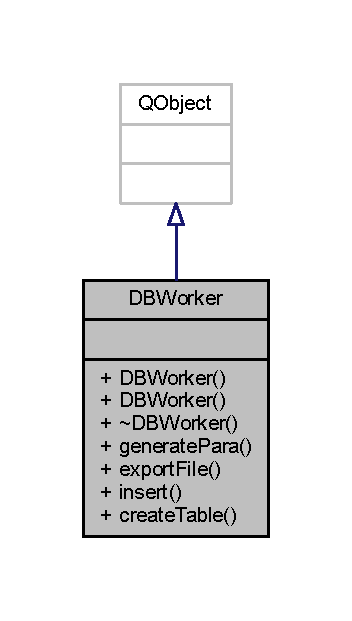
\includegraphics[width=169pt]{class_d_b_worker__inherit__graph}
\end{center}
\end{figure}


D\+B\+Worker 的协作图\+:
\nopagebreak
\begin{figure}[H]
\begin{center}
\leavevmode
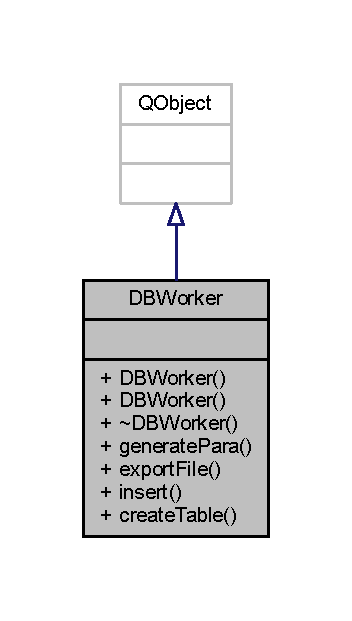
\includegraphics[width=169pt]{class_d_b_worker__coll__graph}
\end{center}
\end{figure}
\subsection*{Public 槽}
\begin{DoxyCompactItemize}
\item 
void \hyperlink{class_d_b_worker_aa71a7eec68cdcec515ec0c11a33865ec}{generate\+Para} ()
\item 
void \hyperlink{class_d_b_worker_a188d324c26f6d112bca1db7f3115262d}{export\+File} (const Q\+String \&table\+Name, const Q\+String \&suffix)
\item 
void \hyperlink{class_d_b_worker_ae56132fc6027e5d06abdc077bcb49fc7}{insert} (const Q\+Date\+Time \&datetime, const Q\+String \&table\+Name)
\item 
void \hyperlink{class_d_b_worker_a37a2193ad84d7276c06795e23b76afa2}{create\+Table} (const Q\+String \&table\+Name)
\end{DoxyCompactItemize}
\subsection*{信号}
\begin{DoxyCompactItemize}
\item 
void \hyperlink{class_d_b_worker_ab89c620df543d5a046626ca64fc64dc1}{export\+Done} ()
\item 
void \hyperlink{class_d_b_worker_a9e1c54915c77ee1aac911ae90a3072cc}{table\+Created} ()
\end{DoxyCompactItemize}
\subsection*{Public 成员函数}
\begin{DoxyCompactItemize}
\item 
\hyperlink{class_d_b_worker_ae87336f36d643f7afc331ba9953b059a}{D\+B\+Worker} (Q\+Object $\ast$parent=0)
\item 
\hyperlink{class_d_b_worker_a23bbf99c73d80b9a6a0cebb332591ae3}{D\+B\+Worker} (qint16 $\ast$buffer)
\item 
\hyperlink{class_d_b_worker_a5b3c98063d26d42c67511fb3f565b9f0}{$\sim$\+D\+B\+Worker} ()
\end{DoxyCompactItemize}


\subsection{构造及析构函数说明}
\index{D\+B\+Worker@{D\+B\+Worker}!D\+B\+Worker@{D\+B\+Worker}}
\index{D\+B\+Worker@{D\+B\+Worker}!D\+B\+Worker@{D\+B\+Worker}}
\subsubsection[{\texorpdfstring{D\+B\+Worker(\+Q\+Object $\ast$parent=0)}{DBWorker(QObject *parent=0)}}]{\setlength{\rightskip}{0pt plus 5cm}D\+B\+Worker\+::\+D\+B\+Worker (
\begin{DoxyParamCaption}
\item[{Q\+Object $\ast$}]{parent = {\ttfamily 0}}
\end{DoxyParamCaption}
)\hspace{0.3cm}{\ttfamily [explicit]}}\hypertarget{class_d_b_worker_ae87336f36d643f7afc331ba9953b059a}{}\label{class_d_b_worker_ae87336f36d643f7afc331ba9953b059a}
\index{D\+B\+Worker@{D\+B\+Worker}!D\+B\+Worker@{D\+B\+Worker}}
\index{D\+B\+Worker@{D\+B\+Worker}!D\+B\+Worker@{D\+B\+Worker}}
\subsubsection[{\texorpdfstring{D\+B\+Worker(qint16 $\ast$buffer)}{DBWorker(qint16 *buffer)}}]{\setlength{\rightskip}{0pt plus 5cm}D\+B\+Worker\+::\+D\+B\+Worker (
\begin{DoxyParamCaption}
\item[{qint16 $\ast$}]{buffer}
\end{DoxyParamCaption}
)}\hypertarget{class_d_b_worker_a23bbf99c73d80b9a6a0cebb332591ae3}{}\label{class_d_b_worker_a23bbf99c73d80b9a6a0cebb332591ae3}
\index{D\+B\+Worker@{D\+B\+Worker}!````~D\+B\+Worker@{$\sim$\+D\+B\+Worker}}
\index{````~D\+B\+Worker@{$\sim$\+D\+B\+Worker}!D\+B\+Worker@{D\+B\+Worker}}
\subsubsection[{\texorpdfstring{$\sim$\+D\+B\+Worker()}{~DBWorker()}}]{\setlength{\rightskip}{0pt plus 5cm}D\+B\+Worker\+::$\sim$\+D\+B\+Worker (
\begin{DoxyParamCaption}
{}
\end{DoxyParamCaption}
)}\hypertarget{class_d_b_worker_a5b3c98063d26d42c67511fb3f565b9f0}{}\label{class_d_b_worker_a5b3c98063d26d42c67511fb3f565b9f0}


\subsection{成员函数说明}
\index{D\+B\+Worker@{D\+B\+Worker}!create\+Table@{create\+Table}}
\index{create\+Table@{create\+Table}!D\+B\+Worker@{D\+B\+Worker}}
\subsubsection[{\texorpdfstring{create\+Table}{createTable}}]{\setlength{\rightskip}{0pt plus 5cm}void D\+B\+Worker\+::create\+Table (
\begin{DoxyParamCaption}
\item[{const Q\+String \&}]{table\+Name}
\end{DoxyParamCaption}
)\hspace{0.3cm}{\ttfamily [slot]}}\hypertarget{class_d_b_worker_a37a2193ad84d7276c06795e23b76afa2}{}\label{class_d_b_worker_a37a2193ad84d7276c06795e23b76afa2}
\index{D\+B\+Worker@{D\+B\+Worker}!export\+Done@{export\+Done}}
\index{export\+Done@{export\+Done}!D\+B\+Worker@{D\+B\+Worker}}
\subsubsection[{\texorpdfstring{export\+Done}{exportDone}}]{\setlength{\rightskip}{0pt plus 5cm}void D\+B\+Worker\+::export\+Done (
\begin{DoxyParamCaption}
{}
\end{DoxyParamCaption}
)\hspace{0.3cm}{\ttfamily [signal]}}\hypertarget{class_d_b_worker_ab89c620df543d5a046626ca64fc64dc1}{}\label{class_d_b_worker_ab89c620df543d5a046626ca64fc64dc1}
\index{D\+B\+Worker@{D\+B\+Worker}!export\+File@{export\+File}}
\index{export\+File@{export\+File}!D\+B\+Worker@{D\+B\+Worker}}
\subsubsection[{\texorpdfstring{export\+File}{exportFile}}]{\setlength{\rightskip}{0pt plus 5cm}void D\+B\+Worker\+::export\+File (
\begin{DoxyParamCaption}
\item[{const Q\+String \&}]{table\+Name, }
\item[{const Q\+String \&}]{suffix}
\end{DoxyParamCaption}
)\hspace{0.3cm}{\ttfamily [slot]}}\hypertarget{class_d_b_worker_a188d324c26f6d112bca1db7f3115262d}{}\label{class_d_b_worker_a188d324c26f6d112bca1db7f3115262d}
\index{D\+B\+Worker@{D\+B\+Worker}!generate\+Para@{generate\+Para}}
\index{generate\+Para@{generate\+Para}!D\+B\+Worker@{D\+B\+Worker}}
\subsubsection[{\texorpdfstring{generate\+Para}{generatePara}}]{\setlength{\rightskip}{0pt plus 5cm}void D\+B\+Worker\+::generate\+Para (
\begin{DoxyParamCaption}
{}
\end{DoxyParamCaption}
)\hspace{0.3cm}{\ttfamily [slot]}}\hypertarget{class_d_b_worker_aa71a7eec68cdcec515ec0c11a33865ec}{}\label{class_d_b_worker_aa71a7eec68cdcec515ec0c11a33865ec}
\index{D\+B\+Worker@{D\+B\+Worker}!insert@{insert}}
\index{insert@{insert}!D\+B\+Worker@{D\+B\+Worker}}
\subsubsection[{\texorpdfstring{insert}{insert}}]{\setlength{\rightskip}{0pt plus 5cm}void D\+B\+Worker\+::insert (
\begin{DoxyParamCaption}
\item[{const Q\+Date\+Time \&}]{datetime, }
\item[{const Q\+String \&}]{table\+Name}
\end{DoxyParamCaption}
)\hspace{0.3cm}{\ttfamily [slot]}}\hypertarget{class_d_b_worker_ae56132fc6027e5d06abdc077bcb49fc7}{}\label{class_d_b_worker_ae56132fc6027e5d06abdc077bcb49fc7}
\index{D\+B\+Worker@{D\+B\+Worker}!table\+Created@{table\+Created}}
\index{table\+Created@{table\+Created}!D\+B\+Worker@{D\+B\+Worker}}
\subsubsection[{\texorpdfstring{table\+Created}{tableCreated}}]{\setlength{\rightskip}{0pt plus 5cm}void D\+B\+Worker\+::table\+Created (
\begin{DoxyParamCaption}
{}
\end{DoxyParamCaption}
)\hspace{0.3cm}{\ttfamily [signal]}}\hypertarget{class_d_b_worker_a9e1c54915c77ee1aac911ae90a3072cc}{}\label{class_d_b_worker_a9e1c54915c77ee1aac911ae90a3072cc}


该类的文档由以下文件生成\+:\begin{DoxyCompactItemize}
\item 
\hyperlink{database_8h}{database.\+h}\item 
\hyperlink{database_8cpp}{database.\+cpp}\end{DoxyCompactItemize}

\hypertarget{class_device}{}\section{Device类 参考}
\label{class_device}\index{Device@{Device}}


{\ttfamily \#include $<$device.\+h$>$}



类 Device 继承关系图\+:
\nopagebreak
\begin{figure}[H]
\begin{center}
\leavevmode
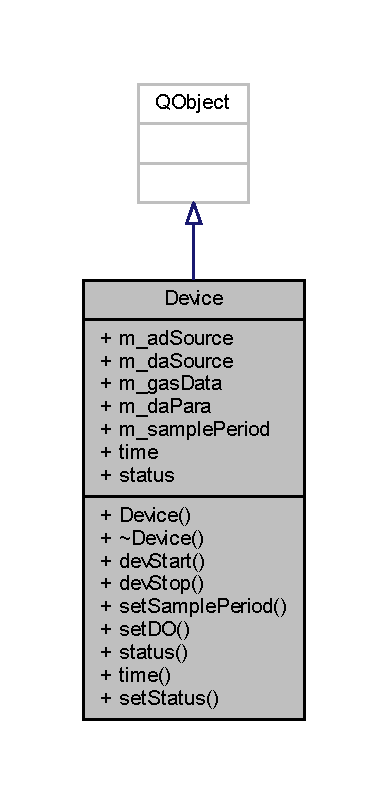
\includegraphics[width=186pt]{class_device__inherit__graph}
\end{center}
\end{figure}


Device 的协作图\+:
\nopagebreak
\begin{figure}[H]
\begin{center}
\leavevmode
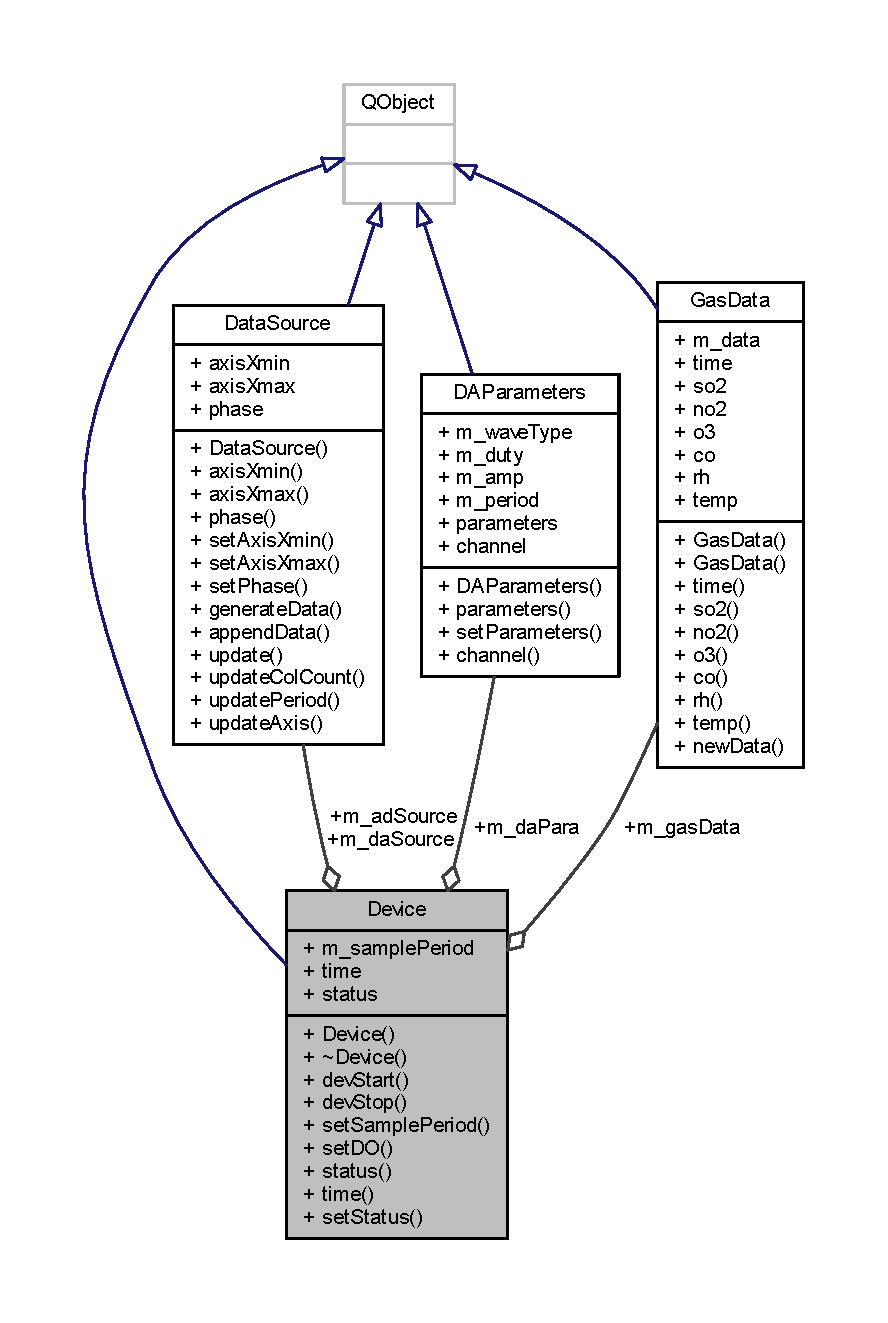
\includegraphics[width=350pt]{class_device__coll__graph}
\end{center}
\end{figure}
\subsection*{Public 槽}
\begin{DoxyCompactItemize}
\item 
void \hyperlink{class_device_a1466fe821dfd974399b09829a1a6ddc5}{set\+Status} (bool s)
\end{DoxyCompactItemize}
\subsection*{信号}
\begin{DoxyCompactItemize}
\item 
void \hyperlink{class_device_a063dbe514cd12d635adbccf38bf4f53f}{status\+Changed} (bool)
\item 
void \hyperlink{class_device_a818f8350ab033557bfb72aef858a0ab7}{time\+Changed} ()
\item 
void \hyperlink{class_device_a1377620e47da1997d012cec27e3c72d4}{acquired} (const Q\+Date\+Time \&)
\item 
void \hyperlink{class_device_a74f0827f51383f85e0cab3ddb81ced4b}{sample\+Period\+Changed} (int)
\item 
void \hyperlink{class_device_afffd72adb7de79c6f9458e0140e04f0c}{heartbeat\+Start} ()
\item 
void \hyperlink{class_device_a0efcae038c0da76b43f9efab5314d200}{heartbeat\+Stop} ()
\item 
void \hyperlink{class_device_a8174b87c354c82e789569b87e7e2591e}{serial\+Close} ()
\end{DoxyCompactItemize}
\subsection*{Public 成员函数}
\begin{DoxyCompactItemize}
\item 
\hyperlink{class_device_acb29365c82264abd26b4cc3239e2fe61}{Device} (qint16 $\ast$buffer)
\item 
\hyperlink{class_device_a9dabc419c8d8df3a686c33ce042bc99a}{$\sim$\+Device} ()
\item 
Q\+\_\+\+I\+N\+V\+O\+K\+A\+B\+LE void \hyperlink{class_device_a68419c7c1d474721cce4f9a0a8b87ba0}{dev\+Start} ()
\item 
Q\+\_\+\+I\+N\+V\+O\+K\+A\+B\+LE void \hyperlink{class_device_a6f87ac6b1a5f7b9fd0fd73adccb460a2}{dev\+Stop} ()
\item 
Q\+\_\+\+I\+N\+V\+O\+K\+A\+B\+LE void \hyperlink{class_device_a4b8abc3bfacc59f46c699b5ead1ea8f8}{set\+Sample\+Period} (int p)
\item 
Q\+\_\+\+I\+N\+V\+O\+K\+A\+B\+LE void \hyperlink{class_device_a5d201e969696bc986fe1f540826e0a8e}{set\+DO} (int indx, bool val)
\item 
bool \hyperlink{class_device_a4953d696fd19d1b45d13dfc857d2bb13}{status} ()
\item 
int \hyperlink{class_device_a0cd70abff838a3fbe695ff74270bcbb5}{time} ()
\end{DoxyCompactItemize}
\subsection*{Public 属性}
\begin{DoxyCompactItemize}
\item 
\hyperlink{class_data_source}{Data\+Source} $\ast$ \hyperlink{class_device_a23b94d39e641579288e476519d5a6e51}{m\+\_\+ad\+Source}
\item 
\hyperlink{class_data_source}{Data\+Source} $\ast$ \hyperlink{class_device_a29f1d7ff9ee32cee8c50b0f3392b5377}{m\+\_\+da\+Source}
\item 
\hyperlink{class_gas_data}{Gas\+Data} $\ast$ \hyperlink{class_device_a4ac8d2530319ebc1b46819db02b59e96}{m\+\_\+gas\+Data}
\item 
\hyperlink{class_d_a_parameters}{D\+A\+Parameters} $\ast$ \hyperlink{class_device_a3f51f6adfa09aa0308d39a88f6378238}{m\+\_\+da\+Para}
\item 
int \hyperlink{class_device_a46fdd5613ae7c31bbb39766230f333a9}{m\+\_\+sample\+Period}
\end{DoxyCompactItemize}
\subsection*{属性}
\begin{DoxyCompactItemize}
\item 
int \hyperlink{class_device_a02388ba20565bf3fb965562dc8a80220}{time}
\item 
bool \hyperlink{class_device_adbc68ead998699f85673fabefda84daf}{status}
\end{DoxyCompactItemize}


\subsection{构造及析构函数说明}
\index{Device@{Device}!Device@{Device}}
\index{Device@{Device}!Device@{Device}}
\subsubsection[{\texorpdfstring{Device(qint16 $\ast$buffer)}{Device(qint16 *buffer)}}]{\setlength{\rightskip}{0pt plus 5cm}Device\+::\+Device (
\begin{DoxyParamCaption}
\item[{qint16 $\ast$}]{buffer}
\end{DoxyParamCaption}
)\hspace{0.3cm}{\ttfamily [explicit]}}\hypertarget{class_device_acb29365c82264abd26b4cc3239e2fe61}{}\label{class_device_acb29365c82264abd26b4cc3239e2fe61}
\index{Device@{Device}!````~Device@{$\sim$\+Device}}
\index{````~Device@{$\sim$\+Device}!Device@{Device}}
\subsubsection[{\texorpdfstring{$\sim$\+Device()}{~Device()}}]{\setlength{\rightskip}{0pt plus 5cm}Device\+::$\sim$\+Device (
\begin{DoxyParamCaption}
{}
\end{DoxyParamCaption}
)}\hypertarget{class_device_a9dabc419c8d8df3a686c33ce042bc99a}{}\label{class_device_a9dabc419c8d8df3a686c33ce042bc99a}


\subsection{成员函数说明}
\index{Device@{Device}!acquired@{acquired}}
\index{acquired@{acquired}!Device@{Device}}
\subsubsection[{\texorpdfstring{acquired}{acquired}}]{\setlength{\rightskip}{0pt plus 5cm}void Device\+::acquired (
\begin{DoxyParamCaption}
\item[{const Q\+Date\+Time \&}]{}
\end{DoxyParamCaption}
)\hspace{0.3cm}{\ttfamily [signal]}}\hypertarget{class_device_a1377620e47da1997d012cec27e3c72d4}{}\label{class_device_a1377620e47da1997d012cec27e3c72d4}
\index{Device@{Device}!dev\+Start@{dev\+Start}}
\index{dev\+Start@{dev\+Start}!Device@{Device}}
\subsubsection[{\texorpdfstring{dev\+Start()}{devStart()}}]{\setlength{\rightskip}{0pt plus 5cm}void Device\+::dev\+Start (
\begin{DoxyParamCaption}
{}
\end{DoxyParamCaption}
)}\hypertarget{class_device_a68419c7c1d474721cce4f9a0a8b87ba0}{}\label{class_device_a68419c7c1d474721cce4f9a0a8b87ba0}
\index{Device@{Device}!dev\+Stop@{dev\+Stop}}
\index{dev\+Stop@{dev\+Stop}!Device@{Device}}
\subsubsection[{\texorpdfstring{dev\+Stop()}{devStop()}}]{\setlength{\rightskip}{0pt plus 5cm}void Device\+::dev\+Stop (
\begin{DoxyParamCaption}
{}
\end{DoxyParamCaption}
)}\hypertarget{class_device_a6f87ac6b1a5f7b9fd0fd73adccb460a2}{}\label{class_device_a6f87ac6b1a5f7b9fd0fd73adccb460a2}
\index{Device@{Device}!heartbeat\+Start@{heartbeat\+Start}}
\index{heartbeat\+Start@{heartbeat\+Start}!Device@{Device}}
\subsubsection[{\texorpdfstring{heartbeat\+Start}{heartbeatStart}}]{\setlength{\rightskip}{0pt plus 5cm}void Device\+::heartbeat\+Start (
\begin{DoxyParamCaption}
{}
\end{DoxyParamCaption}
)\hspace{0.3cm}{\ttfamily [signal]}}\hypertarget{class_device_afffd72adb7de79c6f9458e0140e04f0c}{}\label{class_device_afffd72adb7de79c6f9458e0140e04f0c}
\index{Device@{Device}!heartbeat\+Stop@{heartbeat\+Stop}}
\index{heartbeat\+Stop@{heartbeat\+Stop}!Device@{Device}}
\subsubsection[{\texorpdfstring{heartbeat\+Stop}{heartbeatStop}}]{\setlength{\rightskip}{0pt plus 5cm}void Device\+::heartbeat\+Stop (
\begin{DoxyParamCaption}
{}
\end{DoxyParamCaption}
)\hspace{0.3cm}{\ttfamily [signal]}}\hypertarget{class_device_a0efcae038c0da76b43f9efab5314d200}{}\label{class_device_a0efcae038c0da76b43f9efab5314d200}
\index{Device@{Device}!sample\+Period\+Changed@{sample\+Period\+Changed}}
\index{sample\+Period\+Changed@{sample\+Period\+Changed}!Device@{Device}}
\subsubsection[{\texorpdfstring{sample\+Period\+Changed}{samplePeriodChanged}}]{\setlength{\rightskip}{0pt plus 5cm}void Device\+::sample\+Period\+Changed (
\begin{DoxyParamCaption}
\item[{int}]{}
\end{DoxyParamCaption}
)\hspace{0.3cm}{\ttfamily [signal]}}\hypertarget{class_device_a74f0827f51383f85e0cab3ddb81ced4b}{}\label{class_device_a74f0827f51383f85e0cab3ddb81ced4b}
\index{Device@{Device}!serial\+Close@{serial\+Close}}
\index{serial\+Close@{serial\+Close}!Device@{Device}}
\subsubsection[{\texorpdfstring{serial\+Close}{serialClose}}]{\setlength{\rightskip}{0pt plus 5cm}void Device\+::serial\+Close (
\begin{DoxyParamCaption}
{}
\end{DoxyParamCaption}
)\hspace{0.3cm}{\ttfamily [signal]}}\hypertarget{class_device_a8174b87c354c82e789569b87e7e2591e}{}\label{class_device_a8174b87c354c82e789569b87e7e2591e}
\index{Device@{Device}!set\+DO@{set\+DO}}
\index{set\+DO@{set\+DO}!Device@{Device}}
\subsubsection[{\texorpdfstring{set\+D\+O(int indx, bool val)}{setDO(int indx, bool val)}}]{\setlength{\rightskip}{0pt plus 5cm}void Device\+::set\+DO (
\begin{DoxyParamCaption}
\item[{int}]{indx, }
\item[{bool}]{val}
\end{DoxyParamCaption}
)}\hypertarget{class_device_a5d201e969696bc986fe1f540826e0a8e}{}\label{class_device_a5d201e969696bc986fe1f540826e0a8e}
\index{Device@{Device}!set\+Sample\+Period@{set\+Sample\+Period}}
\index{set\+Sample\+Period@{set\+Sample\+Period}!Device@{Device}}
\subsubsection[{\texorpdfstring{set\+Sample\+Period(int p)}{setSamplePeriod(int p)}}]{\setlength{\rightskip}{0pt plus 5cm}void Device\+::set\+Sample\+Period (
\begin{DoxyParamCaption}
\item[{int}]{p}
\end{DoxyParamCaption}
)}\hypertarget{class_device_a4b8abc3bfacc59f46c699b5ead1ea8f8}{}\label{class_device_a4b8abc3bfacc59f46c699b5ead1ea8f8}
\index{Device@{Device}!set\+Status@{set\+Status}}
\index{set\+Status@{set\+Status}!Device@{Device}}
\subsubsection[{\texorpdfstring{set\+Status}{setStatus}}]{\setlength{\rightskip}{0pt plus 5cm}void Device\+::set\+Status (
\begin{DoxyParamCaption}
\item[{bool}]{s}
\end{DoxyParamCaption}
)\hspace{0.3cm}{\ttfamily [slot]}}\hypertarget{class_device_a1466fe821dfd974399b09829a1a6ddc5}{}\label{class_device_a1466fe821dfd974399b09829a1a6ddc5}
\index{Device@{Device}!status@{status}}
\index{status@{status}!Device@{Device}}
\subsubsection[{\texorpdfstring{status()}{status()}}]{\setlength{\rightskip}{0pt plus 5cm}bool Device\+::status (
\begin{DoxyParamCaption}
{}
\end{DoxyParamCaption}
)}\hypertarget{class_device_a4953d696fd19d1b45d13dfc857d2bb13}{}\label{class_device_a4953d696fd19d1b45d13dfc857d2bb13}
\index{Device@{Device}!status\+Changed@{status\+Changed}}
\index{status\+Changed@{status\+Changed}!Device@{Device}}
\subsubsection[{\texorpdfstring{status\+Changed}{statusChanged}}]{\setlength{\rightskip}{0pt plus 5cm}void Device\+::status\+Changed (
\begin{DoxyParamCaption}
\item[{bool}]{}
\end{DoxyParamCaption}
)\hspace{0.3cm}{\ttfamily [signal]}}\hypertarget{class_device_a063dbe514cd12d635adbccf38bf4f53f}{}\label{class_device_a063dbe514cd12d635adbccf38bf4f53f}
\index{Device@{Device}!time@{time}}
\index{time@{time}!Device@{Device}}
\subsubsection[{\texorpdfstring{time()}{time()}}]{\setlength{\rightskip}{0pt plus 5cm}int Device\+::time (
\begin{DoxyParamCaption}
{}
\end{DoxyParamCaption}
)}\hypertarget{class_device_a0cd70abff838a3fbe695ff74270bcbb5}{}\label{class_device_a0cd70abff838a3fbe695ff74270bcbb5}
\index{Device@{Device}!time\+Changed@{time\+Changed}}
\index{time\+Changed@{time\+Changed}!Device@{Device}}
\subsubsection[{\texorpdfstring{time\+Changed}{timeChanged}}]{\setlength{\rightskip}{0pt plus 5cm}void Device\+::time\+Changed (
\begin{DoxyParamCaption}
{}
\end{DoxyParamCaption}
)\hspace{0.3cm}{\ttfamily [signal]}}\hypertarget{class_device_a818f8350ab033557bfb72aef858a0ab7}{}\label{class_device_a818f8350ab033557bfb72aef858a0ab7}


\subsection{类成员变量说明}
\index{Device@{Device}!m\+\_\+ad\+Source@{m\+\_\+ad\+Source}}
\index{m\+\_\+ad\+Source@{m\+\_\+ad\+Source}!Device@{Device}}
\subsubsection[{\texorpdfstring{m\+\_\+ad\+Source}{m_adSource}}]{\setlength{\rightskip}{0pt plus 5cm}{\bf Data\+Source}$\ast$ Device\+::m\+\_\+ad\+Source}\hypertarget{class_device_a23b94d39e641579288e476519d5a6e51}{}\label{class_device_a23b94d39e641579288e476519d5a6e51}
\index{Device@{Device}!m\+\_\+da\+Para@{m\+\_\+da\+Para}}
\index{m\+\_\+da\+Para@{m\+\_\+da\+Para}!Device@{Device}}
\subsubsection[{\texorpdfstring{m\+\_\+da\+Para}{m_daPara}}]{\setlength{\rightskip}{0pt plus 5cm}{\bf D\+A\+Parameters}$\ast$ Device\+::m\+\_\+da\+Para}\hypertarget{class_device_a3f51f6adfa09aa0308d39a88f6378238}{}\label{class_device_a3f51f6adfa09aa0308d39a88f6378238}
\index{Device@{Device}!m\+\_\+da\+Source@{m\+\_\+da\+Source}}
\index{m\+\_\+da\+Source@{m\+\_\+da\+Source}!Device@{Device}}
\subsubsection[{\texorpdfstring{m\+\_\+da\+Source}{m_daSource}}]{\setlength{\rightskip}{0pt plus 5cm}{\bf Data\+Source}$\ast$ Device\+::m\+\_\+da\+Source}\hypertarget{class_device_a29f1d7ff9ee32cee8c50b0f3392b5377}{}\label{class_device_a29f1d7ff9ee32cee8c50b0f3392b5377}
\index{Device@{Device}!m\+\_\+gas\+Data@{m\+\_\+gas\+Data}}
\index{m\+\_\+gas\+Data@{m\+\_\+gas\+Data}!Device@{Device}}
\subsubsection[{\texorpdfstring{m\+\_\+gas\+Data}{m_gasData}}]{\setlength{\rightskip}{0pt plus 5cm}{\bf Gas\+Data}$\ast$ Device\+::m\+\_\+gas\+Data}\hypertarget{class_device_a4ac8d2530319ebc1b46819db02b59e96}{}\label{class_device_a4ac8d2530319ebc1b46819db02b59e96}
\index{Device@{Device}!m\+\_\+sample\+Period@{m\+\_\+sample\+Period}}
\index{m\+\_\+sample\+Period@{m\+\_\+sample\+Period}!Device@{Device}}
\subsubsection[{\texorpdfstring{m\+\_\+sample\+Period}{m_samplePeriod}}]{\setlength{\rightskip}{0pt plus 5cm}int Device\+::m\+\_\+sample\+Period}\hypertarget{class_device_a46fdd5613ae7c31bbb39766230f333a9}{}\label{class_device_a46fdd5613ae7c31bbb39766230f333a9}


\subsection{属性说明}
\index{Device@{Device}!status@{status}}
\index{status@{status}!Device@{Device}}
\subsubsection[{\texorpdfstring{status}{status}}]{\setlength{\rightskip}{0pt plus 5cm}bool Device\+::status\hspace{0.3cm}{\ttfamily [read]}, {\ttfamily [write]}}\hypertarget{class_device_adbc68ead998699f85673fabefda84daf}{}\label{class_device_adbc68ead998699f85673fabefda84daf}
\index{Device@{Device}!time@{time}}
\index{time@{time}!Device@{Device}}
\subsubsection[{\texorpdfstring{time}{time}}]{\setlength{\rightskip}{0pt plus 5cm}int Device\+::time\hspace{0.3cm}{\ttfamily [read]}}\hypertarget{class_device_a02388ba20565bf3fb965562dc8a80220}{}\label{class_device_a02388ba20565bf3fb965562dc8a80220}


该类的文档由以下文件生成\+:\begin{DoxyCompactItemize}
\item 
\hyperlink{device_8h}{device.\+h}\item 
\hyperlink{device_8cpp}{device.\+cpp}\end{DoxyCompactItemize}

\hypertarget{class_gas_data}{}\section{Gas\+Data类 参考}
\label{class_gas_data}\index{Gas\+Data@{Gas\+Data}}


{\ttfamily \#include $<$gasdata.\+h$>$}



类 Gas\+Data 继承关系图\+:
\nopagebreak
\begin{figure}[H]
\begin{center}
\leavevmode
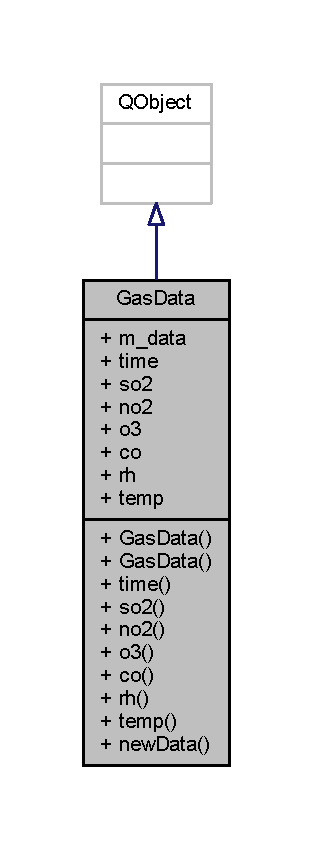
\includegraphics[width=150pt]{class_gas_data__inherit__graph}
\end{center}
\end{figure}


Gas\+Data 的协作图\+:
\nopagebreak
\begin{figure}[H]
\begin{center}
\leavevmode
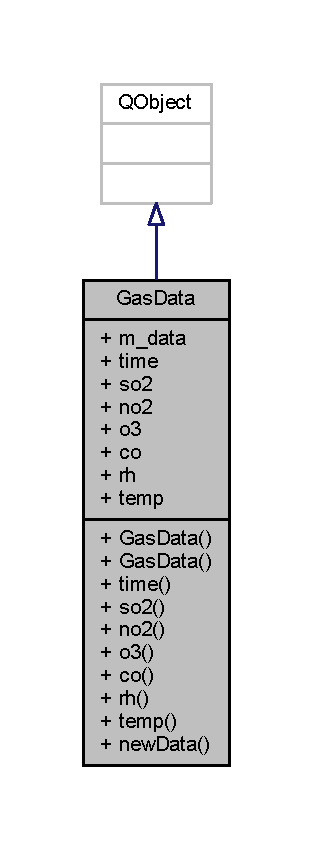
\includegraphics[width=150pt]{class_gas_data__coll__graph}
\end{center}
\end{figure}
\subsection*{Public 槽}
\begin{DoxyCompactItemize}
\item 
void \hyperlink{class_gas_data_a3f73b70a55cf1f7b39099500cacb9e13}{new\+Data} ()
\end{DoxyCompactItemize}
\subsection*{信号}
\begin{DoxyCompactItemize}
\item 
void \hyperlink{class_gas_data_a0b0142d54233b7c659c3677a98ac6408}{time\+Changed} ()
\item 
void \hyperlink{class_gas_data_a88c01ec0f19987e146e488f3b797c415}{so2\+Changed} ()
\item 
void \hyperlink{class_gas_data_af274f1190089b70ef37f29cd0f99cf98}{no2\+Changed} ()
\item 
void \hyperlink{class_gas_data_a6ae59169bddd89f6d5a343e09d0fafb9}{co\+Changed} ()
\item 
void \hyperlink{class_gas_data_a0dbd3935dd960ee64f923b289da91534}{o3\+Changed} ()
\item 
void \hyperlink{class_gas_data_aca9ccae43ed434f654b2bdd785ba5088}{rh\+Changed} ()
\item 
void \hyperlink{class_gas_data_a99353a1207bea33ba06d5f36c0607c56}{temp\+Changed} ()
\item 
void \hyperlink{class_gas_data_af2b0284599635c7eecdb221d5b2b4f14}{data\+Updated} ()
\end{DoxyCompactItemize}
\subsection*{Public 成员函数}
\begin{DoxyCompactItemize}
\item 
\hyperlink{class_gas_data_ad2c93e20d8bc78ed424620a7cda0eaf3}{Gas\+Data} (Q\+Object $\ast$parent=0)
\item 
\hyperlink{class_gas_data_af8180388cf3d05085350be220defcfe6}{Gas\+Data} (qint16 $\ast$buffer)
\item 
qreal \hyperlink{class_gas_data_a0bd45899366f0c1aef068ff36e58cf40}{time} ()
\item 
qreal \hyperlink{class_gas_data_a1bb0e9b83b219aee6056cba5b95d6e57}{so2} ()
\item 
qreal \hyperlink{class_gas_data_ab60937b48c6f7bb235ac039ca144e1dc}{no2} ()
\item 
qreal \hyperlink{class_gas_data_a96adbc847434323af3b5d9f519d3897e}{o3} ()
\item 
qreal \hyperlink{class_gas_data_a0b28ed478992c372ea7a4f78e4c2435f}{co} ()
\item 
qreal \hyperlink{class_gas_data_a12dbcfe821d2c16caf9743842dc3ef4a}{rh} ()
\item 
qreal \hyperlink{class_gas_data_a5841654a877a78d2e511d0c47d931f45}{temp} ()
\end{DoxyCompactItemize}
\subsection*{Public 属性}
\begin{DoxyCompactItemize}
\item 
Q\+List$<$ qreal $>$ \hyperlink{class_gas_data_a9a9580213b02c5be6f69016afc12f714}{m\+\_\+data}
\end{DoxyCompactItemize}
\subsection*{属性}
\begin{DoxyCompactItemize}
\item 
qreal \hyperlink{class_gas_data_adc494c358095749e8548c282c7e83cb2}{time}
\item 
qreal \hyperlink{class_gas_data_af793f7ce28e6253cde7e64157085a78d}{so2}
\item 
qreal \hyperlink{class_gas_data_ac639f2784cc5928b18698719100ec4e4}{no2}
\item 
qreal \hyperlink{class_gas_data_a3d5fdde02a26dff391b676b8fbe13a2d}{o3}
\item 
qreal \hyperlink{class_gas_data_aec8d615eb86254833ed796edcf8a8221}{co}
\item 
qreal \hyperlink{class_gas_data_a521479d6e53eeac6c5f8b61479c7e383}{rh}
\item 
qreal \hyperlink{class_gas_data_a00dfe6cd501e6bb0dcb555b5e3f1bbf2}{temp}
\end{DoxyCompactItemize}


\subsection{构造及析构函数说明}
\index{Gas\+Data@{Gas\+Data}!Gas\+Data@{Gas\+Data}}
\index{Gas\+Data@{Gas\+Data}!Gas\+Data@{Gas\+Data}}
\subsubsection[{\texorpdfstring{Gas\+Data(\+Q\+Object $\ast$parent=0)}{GasData(QObject *parent=0)}}]{\setlength{\rightskip}{0pt plus 5cm}Gas\+Data\+::\+Gas\+Data (
\begin{DoxyParamCaption}
\item[{Q\+Object $\ast$}]{parent = {\ttfamily 0}}
\end{DoxyParamCaption}
)\hspace{0.3cm}{\ttfamily [explicit]}}\hypertarget{class_gas_data_ad2c93e20d8bc78ed424620a7cda0eaf3}{}\label{class_gas_data_ad2c93e20d8bc78ed424620a7cda0eaf3}
\index{Gas\+Data@{Gas\+Data}!Gas\+Data@{Gas\+Data}}
\index{Gas\+Data@{Gas\+Data}!Gas\+Data@{Gas\+Data}}
\subsubsection[{\texorpdfstring{Gas\+Data(qint16 $\ast$buffer)}{GasData(qint16 *buffer)}}]{\setlength{\rightskip}{0pt plus 5cm}Gas\+Data\+::\+Gas\+Data (
\begin{DoxyParamCaption}
\item[{qint16 $\ast$}]{buffer}
\end{DoxyParamCaption}
)}\hypertarget{class_gas_data_af8180388cf3d05085350be220defcfe6}{}\label{class_gas_data_af8180388cf3d05085350be220defcfe6}


\subsection{成员函数说明}
\index{Gas\+Data@{Gas\+Data}!co@{co}}
\index{co@{co}!Gas\+Data@{Gas\+Data}}
\subsubsection[{\texorpdfstring{co()}{co()}}]{\setlength{\rightskip}{0pt plus 5cm}qreal Gas\+Data\+::co (
\begin{DoxyParamCaption}
{}
\end{DoxyParamCaption}
)}\hypertarget{class_gas_data_a0b28ed478992c372ea7a4f78e4c2435f}{}\label{class_gas_data_a0b28ed478992c372ea7a4f78e4c2435f}
\index{Gas\+Data@{Gas\+Data}!co\+Changed@{co\+Changed}}
\index{co\+Changed@{co\+Changed}!Gas\+Data@{Gas\+Data}}
\subsubsection[{\texorpdfstring{co\+Changed}{coChanged}}]{\setlength{\rightskip}{0pt plus 5cm}void Gas\+Data\+::co\+Changed (
\begin{DoxyParamCaption}
{}
\end{DoxyParamCaption}
)\hspace{0.3cm}{\ttfamily [signal]}}\hypertarget{class_gas_data_a6ae59169bddd89f6d5a343e09d0fafb9}{}\label{class_gas_data_a6ae59169bddd89f6d5a343e09d0fafb9}
\index{Gas\+Data@{Gas\+Data}!data\+Updated@{data\+Updated}}
\index{data\+Updated@{data\+Updated}!Gas\+Data@{Gas\+Data}}
\subsubsection[{\texorpdfstring{data\+Updated}{dataUpdated}}]{\setlength{\rightskip}{0pt plus 5cm}void Gas\+Data\+::data\+Updated (
\begin{DoxyParamCaption}
{}
\end{DoxyParamCaption}
)\hspace{0.3cm}{\ttfamily [signal]}}\hypertarget{class_gas_data_af2b0284599635c7eecdb221d5b2b4f14}{}\label{class_gas_data_af2b0284599635c7eecdb221d5b2b4f14}
\index{Gas\+Data@{Gas\+Data}!new\+Data@{new\+Data}}
\index{new\+Data@{new\+Data}!Gas\+Data@{Gas\+Data}}
\subsubsection[{\texorpdfstring{new\+Data}{newData}}]{\setlength{\rightskip}{0pt plus 5cm}void Gas\+Data\+::new\+Data (
\begin{DoxyParamCaption}
{}
\end{DoxyParamCaption}
)\hspace{0.3cm}{\ttfamily [slot]}}\hypertarget{class_gas_data_a3f73b70a55cf1f7b39099500cacb9e13}{}\label{class_gas_data_a3f73b70a55cf1f7b39099500cacb9e13}
\index{Gas\+Data@{Gas\+Data}!no2@{no2}}
\index{no2@{no2}!Gas\+Data@{Gas\+Data}}
\subsubsection[{\texorpdfstring{no2()}{no2()}}]{\setlength{\rightskip}{0pt plus 5cm}qreal Gas\+Data\+::no2 (
\begin{DoxyParamCaption}
{}
\end{DoxyParamCaption}
)}\hypertarget{class_gas_data_ab60937b48c6f7bb235ac039ca144e1dc}{}\label{class_gas_data_ab60937b48c6f7bb235ac039ca144e1dc}
\index{Gas\+Data@{Gas\+Data}!no2\+Changed@{no2\+Changed}}
\index{no2\+Changed@{no2\+Changed}!Gas\+Data@{Gas\+Data}}
\subsubsection[{\texorpdfstring{no2\+Changed}{no2Changed}}]{\setlength{\rightskip}{0pt plus 5cm}void Gas\+Data\+::no2\+Changed (
\begin{DoxyParamCaption}
{}
\end{DoxyParamCaption}
)\hspace{0.3cm}{\ttfamily [signal]}}\hypertarget{class_gas_data_af274f1190089b70ef37f29cd0f99cf98}{}\label{class_gas_data_af274f1190089b70ef37f29cd0f99cf98}
\index{Gas\+Data@{Gas\+Data}!o3@{o3}}
\index{o3@{o3}!Gas\+Data@{Gas\+Data}}
\subsubsection[{\texorpdfstring{o3()}{o3()}}]{\setlength{\rightskip}{0pt plus 5cm}qreal Gas\+Data\+::o3 (
\begin{DoxyParamCaption}
{}
\end{DoxyParamCaption}
)}\hypertarget{class_gas_data_a96adbc847434323af3b5d9f519d3897e}{}\label{class_gas_data_a96adbc847434323af3b5d9f519d3897e}
\index{Gas\+Data@{Gas\+Data}!o3\+Changed@{o3\+Changed}}
\index{o3\+Changed@{o3\+Changed}!Gas\+Data@{Gas\+Data}}
\subsubsection[{\texorpdfstring{o3\+Changed}{o3Changed}}]{\setlength{\rightskip}{0pt plus 5cm}void Gas\+Data\+::o3\+Changed (
\begin{DoxyParamCaption}
{}
\end{DoxyParamCaption}
)\hspace{0.3cm}{\ttfamily [signal]}}\hypertarget{class_gas_data_a0dbd3935dd960ee64f923b289da91534}{}\label{class_gas_data_a0dbd3935dd960ee64f923b289da91534}
\index{Gas\+Data@{Gas\+Data}!rh@{rh}}
\index{rh@{rh}!Gas\+Data@{Gas\+Data}}
\subsubsection[{\texorpdfstring{rh()}{rh()}}]{\setlength{\rightskip}{0pt plus 5cm}qreal Gas\+Data\+::rh (
\begin{DoxyParamCaption}
{}
\end{DoxyParamCaption}
)}\hypertarget{class_gas_data_a12dbcfe821d2c16caf9743842dc3ef4a}{}\label{class_gas_data_a12dbcfe821d2c16caf9743842dc3ef4a}
\index{Gas\+Data@{Gas\+Data}!rh\+Changed@{rh\+Changed}}
\index{rh\+Changed@{rh\+Changed}!Gas\+Data@{Gas\+Data}}
\subsubsection[{\texorpdfstring{rh\+Changed}{rhChanged}}]{\setlength{\rightskip}{0pt plus 5cm}void Gas\+Data\+::rh\+Changed (
\begin{DoxyParamCaption}
{}
\end{DoxyParamCaption}
)\hspace{0.3cm}{\ttfamily [signal]}}\hypertarget{class_gas_data_aca9ccae43ed434f654b2bdd785ba5088}{}\label{class_gas_data_aca9ccae43ed434f654b2bdd785ba5088}
\index{Gas\+Data@{Gas\+Data}!so2@{so2}}
\index{so2@{so2}!Gas\+Data@{Gas\+Data}}
\subsubsection[{\texorpdfstring{so2()}{so2()}}]{\setlength{\rightskip}{0pt plus 5cm}qreal Gas\+Data\+::so2 (
\begin{DoxyParamCaption}
{}
\end{DoxyParamCaption}
)}\hypertarget{class_gas_data_a1bb0e9b83b219aee6056cba5b95d6e57}{}\label{class_gas_data_a1bb0e9b83b219aee6056cba5b95d6e57}
\index{Gas\+Data@{Gas\+Data}!so2\+Changed@{so2\+Changed}}
\index{so2\+Changed@{so2\+Changed}!Gas\+Data@{Gas\+Data}}
\subsubsection[{\texorpdfstring{so2\+Changed}{so2Changed}}]{\setlength{\rightskip}{0pt plus 5cm}void Gas\+Data\+::so2\+Changed (
\begin{DoxyParamCaption}
{}
\end{DoxyParamCaption}
)\hspace{0.3cm}{\ttfamily [signal]}}\hypertarget{class_gas_data_a88c01ec0f19987e146e488f3b797c415}{}\label{class_gas_data_a88c01ec0f19987e146e488f3b797c415}
\index{Gas\+Data@{Gas\+Data}!temp@{temp}}
\index{temp@{temp}!Gas\+Data@{Gas\+Data}}
\subsubsection[{\texorpdfstring{temp()}{temp()}}]{\setlength{\rightskip}{0pt plus 5cm}qreal Gas\+Data\+::temp (
\begin{DoxyParamCaption}
{}
\end{DoxyParamCaption}
)}\hypertarget{class_gas_data_a5841654a877a78d2e511d0c47d931f45}{}\label{class_gas_data_a5841654a877a78d2e511d0c47d931f45}
\index{Gas\+Data@{Gas\+Data}!temp\+Changed@{temp\+Changed}}
\index{temp\+Changed@{temp\+Changed}!Gas\+Data@{Gas\+Data}}
\subsubsection[{\texorpdfstring{temp\+Changed}{tempChanged}}]{\setlength{\rightskip}{0pt plus 5cm}void Gas\+Data\+::temp\+Changed (
\begin{DoxyParamCaption}
{}
\end{DoxyParamCaption}
)\hspace{0.3cm}{\ttfamily [signal]}}\hypertarget{class_gas_data_a99353a1207bea33ba06d5f36c0607c56}{}\label{class_gas_data_a99353a1207bea33ba06d5f36c0607c56}
\index{Gas\+Data@{Gas\+Data}!time@{time}}
\index{time@{time}!Gas\+Data@{Gas\+Data}}
\subsubsection[{\texorpdfstring{time()}{time()}}]{\setlength{\rightskip}{0pt plus 5cm}qreal Gas\+Data\+::time (
\begin{DoxyParamCaption}
{}
\end{DoxyParamCaption}
)}\hypertarget{class_gas_data_a0bd45899366f0c1aef068ff36e58cf40}{}\label{class_gas_data_a0bd45899366f0c1aef068ff36e58cf40}
\index{Gas\+Data@{Gas\+Data}!time\+Changed@{time\+Changed}}
\index{time\+Changed@{time\+Changed}!Gas\+Data@{Gas\+Data}}
\subsubsection[{\texorpdfstring{time\+Changed}{timeChanged}}]{\setlength{\rightskip}{0pt plus 5cm}void Gas\+Data\+::time\+Changed (
\begin{DoxyParamCaption}
{}
\end{DoxyParamCaption}
)\hspace{0.3cm}{\ttfamily [signal]}}\hypertarget{class_gas_data_a0b0142d54233b7c659c3677a98ac6408}{}\label{class_gas_data_a0b0142d54233b7c659c3677a98ac6408}


\subsection{类成员变量说明}
\index{Gas\+Data@{Gas\+Data}!m\+\_\+data@{m\+\_\+data}}
\index{m\+\_\+data@{m\+\_\+data}!Gas\+Data@{Gas\+Data}}
\subsubsection[{\texorpdfstring{m\+\_\+data}{m_data}}]{\setlength{\rightskip}{0pt plus 5cm}Q\+List$<$qreal$>$ Gas\+Data\+::m\+\_\+data}\hypertarget{class_gas_data_a9a9580213b02c5be6f69016afc12f714}{}\label{class_gas_data_a9a9580213b02c5be6f69016afc12f714}


\subsection{属性说明}
\index{Gas\+Data@{Gas\+Data}!co@{co}}
\index{co@{co}!Gas\+Data@{Gas\+Data}}
\subsubsection[{\texorpdfstring{co}{co}}]{\setlength{\rightskip}{0pt plus 5cm}qreal Gas\+Data\+::co\hspace{0.3cm}{\ttfamily [read]}}\hypertarget{class_gas_data_aec8d615eb86254833ed796edcf8a8221}{}\label{class_gas_data_aec8d615eb86254833ed796edcf8a8221}
\index{Gas\+Data@{Gas\+Data}!no2@{no2}}
\index{no2@{no2}!Gas\+Data@{Gas\+Data}}
\subsubsection[{\texorpdfstring{no2}{no2}}]{\setlength{\rightskip}{0pt plus 5cm}qreal Gas\+Data\+::no2\hspace{0.3cm}{\ttfamily [read]}}\hypertarget{class_gas_data_ac639f2784cc5928b18698719100ec4e4}{}\label{class_gas_data_ac639f2784cc5928b18698719100ec4e4}
\index{Gas\+Data@{Gas\+Data}!o3@{o3}}
\index{o3@{o3}!Gas\+Data@{Gas\+Data}}
\subsubsection[{\texorpdfstring{o3}{o3}}]{\setlength{\rightskip}{0pt plus 5cm}qreal Gas\+Data\+::o3\hspace{0.3cm}{\ttfamily [read]}}\hypertarget{class_gas_data_a3d5fdde02a26dff391b676b8fbe13a2d}{}\label{class_gas_data_a3d5fdde02a26dff391b676b8fbe13a2d}
\index{Gas\+Data@{Gas\+Data}!rh@{rh}}
\index{rh@{rh}!Gas\+Data@{Gas\+Data}}
\subsubsection[{\texorpdfstring{rh}{rh}}]{\setlength{\rightskip}{0pt plus 5cm}qreal Gas\+Data\+::rh\hspace{0.3cm}{\ttfamily [read]}}\hypertarget{class_gas_data_a521479d6e53eeac6c5f8b61479c7e383}{}\label{class_gas_data_a521479d6e53eeac6c5f8b61479c7e383}
\index{Gas\+Data@{Gas\+Data}!so2@{so2}}
\index{so2@{so2}!Gas\+Data@{Gas\+Data}}
\subsubsection[{\texorpdfstring{so2}{so2}}]{\setlength{\rightskip}{0pt plus 5cm}qreal Gas\+Data\+::so2\hspace{0.3cm}{\ttfamily [read]}}\hypertarget{class_gas_data_af793f7ce28e6253cde7e64157085a78d}{}\label{class_gas_data_af793f7ce28e6253cde7e64157085a78d}
\index{Gas\+Data@{Gas\+Data}!temp@{temp}}
\index{temp@{temp}!Gas\+Data@{Gas\+Data}}
\subsubsection[{\texorpdfstring{temp}{temp}}]{\setlength{\rightskip}{0pt plus 5cm}qreal Gas\+Data\+::temp\hspace{0.3cm}{\ttfamily [read]}}\hypertarget{class_gas_data_a00dfe6cd501e6bb0dcb555b5e3f1bbf2}{}\label{class_gas_data_a00dfe6cd501e6bb0dcb555b5e3f1bbf2}
\index{Gas\+Data@{Gas\+Data}!time@{time}}
\index{time@{time}!Gas\+Data@{Gas\+Data}}
\subsubsection[{\texorpdfstring{time}{time}}]{\setlength{\rightskip}{0pt plus 5cm}qreal Gas\+Data\+::time\hspace{0.3cm}{\ttfamily [read]}}\hypertarget{class_gas_data_adc494c358095749e8548c282c7e83cb2}{}\label{class_gas_data_adc494c358095749e8548c282c7e83cb2}


该类的文档由以下文件生成\+:\begin{DoxyCompactItemize}
\item 
\hyperlink{gasdata_8h}{gasdata.\+h}\item 
\hyperlink{gasdata_8cpp}{gasdata.\+cpp}\end{DoxyCompactItemize}

\hypertarget{class_serial}{}\section{Serial类 参考}
\label{class_serial}\index{Serial@{Serial}}


{\ttfamily \#include $<$serial.\+h$>$}



类 Serial 继承关系图\+:
\nopagebreak
\begin{figure}[H]
\begin{center}
\leavevmode
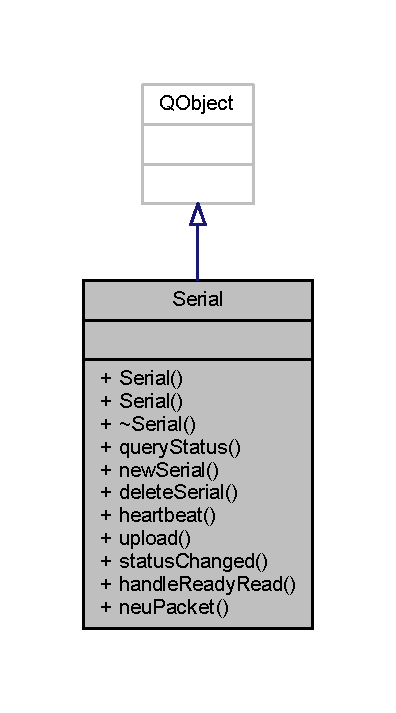
\includegraphics[width=190pt]{class_serial__inherit__graph}
\end{center}
\end{figure}


Serial 的协作图\+:
\nopagebreak
\begin{figure}[H]
\begin{center}
\leavevmode
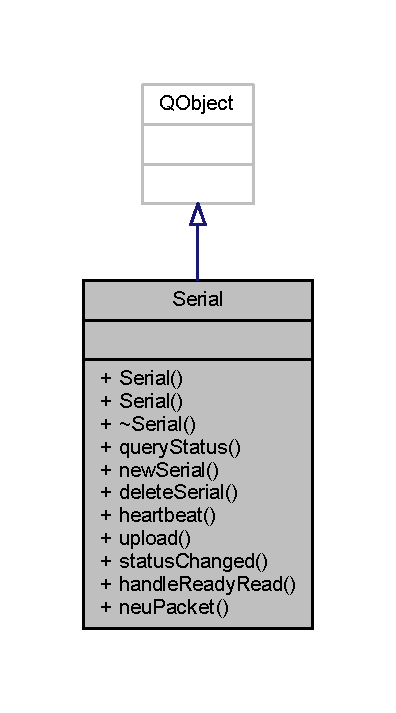
\includegraphics[width=190pt]{class_serial__coll__graph}
\end{center}
\end{figure}
\subsection*{Public 槽}
\begin{DoxyCompactItemize}
\item 
void \hyperlink{class_serial_af6d54e816b6ecdb4c9591a358dbd5bba}{new\+Serial} ()
\item 
void \hyperlink{class_serial_a518ed82ddf35ec61ea9a2f6eeb5dbbca}{delete\+Serial} ()
\item 
void \hyperlink{class_serial_a99aebe8e75cc2074d071a4cdf770055f}{heartbeat} ()
\item 
void \hyperlink{class_serial_aa4ac5bea11414ef5f7e0380674a93d92}{upload} ()
\item 
void \hyperlink{class_serial_a86b9ae52feeb06df6f26b7aeb2203573}{status\+Changed} (bool s)
\item 
void \hyperlink{class_serial_a7d1a32468b83b21ccd377675c72908a2}{handle\+Ready\+Read} ()
\item 
void \hyperlink{class_serial_a3cf77ae7d445be45fe265474db2fa104}{neu\+Packet} (Q\+Byte\+Array const \&d)
\end{DoxyCompactItemize}
\subsection*{信号}
\begin{DoxyCompactItemize}
\item 
void \hyperlink{class_serial_ab7458d9ecc6c44071563f00d027e58f3}{status\+Update} (bool)
\item 
void \hyperlink{class_serial_a39981427dda0ddaedbecff23d1b44ef9}{close\+Serial} ()
\end{DoxyCompactItemize}
\subsection*{Public 成员函数}
\begin{DoxyCompactItemize}
\item 
\hyperlink{class_serial_a994a3a6972a06a34b8231ec5f2223b46}{Serial} (Q\+Object $\ast$parent=0)
\item 
\hyperlink{class_serial_a379cf1950618d1197d90668d5305dbf8}{Serial} (int id, Q\+List$<$ qreal $>$ $\ast$data, Q\+Object $\ast$parent=0)
\item 
\hyperlink{class_serial_a5b32c394c0ff923a4ef1c13cfb20a6ba}{$\sim$\+Serial} ()
\item 
void \hyperlink{class_serial_a44ac0f4e8c2bdb5d6cb31a7f263f6b23}{query\+Status} (int code=3)
\end{DoxyCompactItemize}


\subsection{构造及析构函数说明}
\index{Serial@{Serial}!Serial@{Serial}}
\index{Serial@{Serial}!Serial@{Serial}}
\subsubsection[{\texorpdfstring{Serial(\+Q\+Object $\ast$parent=0)}{Serial(QObject *parent=0)}}]{\setlength{\rightskip}{0pt plus 5cm}Serial\+::\+Serial (
\begin{DoxyParamCaption}
\item[{Q\+Object $\ast$}]{parent = {\ttfamily 0}}
\end{DoxyParamCaption}
)\hspace{0.3cm}{\ttfamily [explicit]}}\hypertarget{class_serial_a994a3a6972a06a34b8231ec5f2223b46}{}\label{class_serial_a994a3a6972a06a34b8231ec5f2223b46}
\index{Serial@{Serial}!Serial@{Serial}}
\index{Serial@{Serial}!Serial@{Serial}}
\subsubsection[{\texorpdfstring{Serial(int id, Q\+List$<$ qreal $>$ $\ast$data, Q\+Object $\ast$parent=0)}{Serial(int id, QList< qreal > *data, QObject *parent=0)}}]{\setlength{\rightskip}{0pt plus 5cm}Serial\+::\+Serial (
\begin{DoxyParamCaption}
\item[{int}]{id, }
\item[{Q\+List$<$ qreal $>$ $\ast$}]{data, }
\item[{Q\+Object $\ast$}]{parent = {\ttfamily 0}}
\end{DoxyParamCaption}
)}\hypertarget{class_serial_a379cf1950618d1197d90668d5305dbf8}{}\label{class_serial_a379cf1950618d1197d90668d5305dbf8}
\index{Serial@{Serial}!````~Serial@{$\sim$\+Serial}}
\index{````~Serial@{$\sim$\+Serial}!Serial@{Serial}}
\subsubsection[{\texorpdfstring{$\sim$\+Serial()}{~Serial()}}]{\setlength{\rightskip}{0pt plus 5cm}Serial\+::$\sim$\+Serial (
\begin{DoxyParamCaption}
{}
\end{DoxyParamCaption}
)}\hypertarget{class_serial_a5b32c394c0ff923a4ef1c13cfb20a6ba}{}\label{class_serial_a5b32c394c0ff923a4ef1c13cfb20a6ba}


\subsection{成员函数说明}
\index{Serial@{Serial}!close\+Serial@{close\+Serial}}
\index{close\+Serial@{close\+Serial}!Serial@{Serial}}
\subsubsection[{\texorpdfstring{close\+Serial}{closeSerial}}]{\setlength{\rightskip}{0pt plus 5cm}void Serial\+::close\+Serial (
\begin{DoxyParamCaption}
{}
\end{DoxyParamCaption}
)\hspace{0.3cm}{\ttfamily [signal]}}\hypertarget{class_serial_a39981427dda0ddaedbecff23d1b44ef9}{}\label{class_serial_a39981427dda0ddaedbecff23d1b44ef9}
\index{Serial@{Serial}!delete\+Serial@{delete\+Serial}}
\index{delete\+Serial@{delete\+Serial}!Serial@{Serial}}
\subsubsection[{\texorpdfstring{delete\+Serial}{deleteSerial}}]{\setlength{\rightskip}{0pt plus 5cm}void Serial\+::delete\+Serial (
\begin{DoxyParamCaption}
{}
\end{DoxyParamCaption}
)\hspace{0.3cm}{\ttfamily [slot]}}\hypertarget{class_serial_a518ed82ddf35ec61ea9a2f6eeb5dbbca}{}\label{class_serial_a518ed82ddf35ec61ea9a2f6eeb5dbbca}
\index{Serial@{Serial}!handle\+Ready\+Read@{handle\+Ready\+Read}}
\index{handle\+Ready\+Read@{handle\+Ready\+Read}!Serial@{Serial}}
\subsubsection[{\texorpdfstring{handle\+Ready\+Read}{handleReadyRead}}]{\setlength{\rightskip}{0pt plus 5cm}void Serial\+::handle\+Ready\+Read (
\begin{DoxyParamCaption}
{}
\end{DoxyParamCaption}
)\hspace{0.3cm}{\ttfamily [slot]}}\hypertarget{class_serial_a7d1a32468b83b21ccd377675c72908a2}{}\label{class_serial_a7d1a32468b83b21ccd377675c72908a2}
\index{Serial@{Serial}!heartbeat@{heartbeat}}
\index{heartbeat@{heartbeat}!Serial@{Serial}}
\subsubsection[{\texorpdfstring{heartbeat}{heartbeat}}]{\setlength{\rightskip}{0pt plus 5cm}void Serial\+::heartbeat (
\begin{DoxyParamCaption}
{}
\end{DoxyParamCaption}
)\hspace{0.3cm}{\ttfamily [slot]}}\hypertarget{class_serial_a99aebe8e75cc2074d071a4cdf770055f}{}\label{class_serial_a99aebe8e75cc2074d071a4cdf770055f}
\index{Serial@{Serial}!neu\+Packet@{neu\+Packet}}
\index{neu\+Packet@{neu\+Packet}!Serial@{Serial}}
\subsubsection[{\texorpdfstring{neu\+Packet}{neuPacket}}]{\setlength{\rightskip}{0pt plus 5cm}void Serial\+::neu\+Packet (
\begin{DoxyParamCaption}
\item[{Q\+Byte\+Array const \&}]{d}
\end{DoxyParamCaption}
)\hspace{0.3cm}{\ttfamily [slot]}}\hypertarget{class_serial_a3cf77ae7d445be45fe265474db2fa104}{}\label{class_serial_a3cf77ae7d445be45fe265474db2fa104}
\index{Serial@{Serial}!new\+Serial@{new\+Serial}}
\index{new\+Serial@{new\+Serial}!Serial@{Serial}}
\subsubsection[{\texorpdfstring{new\+Serial}{newSerial}}]{\setlength{\rightskip}{0pt plus 5cm}void Serial\+::new\+Serial (
\begin{DoxyParamCaption}
{}
\end{DoxyParamCaption}
)\hspace{0.3cm}{\ttfamily [slot]}}\hypertarget{class_serial_af6d54e816b6ecdb4c9591a358dbd5bba}{}\label{class_serial_af6d54e816b6ecdb4c9591a358dbd5bba}
\index{Serial@{Serial}!query\+Status@{query\+Status}}
\index{query\+Status@{query\+Status}!Serial@{Serial}}
\subsubsection[{\texorpdfstring{query\+Status(int code=3)}{queryStatus(int code=3)}}]{\setlength{\rightskip}{0pt plus 5cm}void Serial\+::query\+Status (
\begin{DoxyParamCaption}
\item[{int}]{code = {\ttfamily 3}}
\end{DoxyParamCaption}
)}\hypertarget{class_serial_a44ac0f4e8c2bdb5d6cb31a7f263f6b23}{}\label{class_serial_a44ac0f4e8c2bdb5d6cb31a7f263f6b23}
\index{Serial@{Serial}!status\+Changed@{status\+Changed}}
\index{status\+Changed@{status\+Changed}!Serial@{Serial}}
\subsubsection[{\texorpdfstring{status\+Changed}{statusChanged}}]{\setlength{\rightskip}{0pt plus 5cm}void Serial\+::status\+Changed (
\begin{DoxyParamCaption}
\item[{bool}]{s}
\end{DoxyParamCaption}
)\hspace{0.3cm}{\ttfamily [slot]}}\hypertarget{class_serial_a86b9ae52feeb06df6f26b7aeb2203573}{}\label{class_serial_a86b9ae52feeb06df6f26b7aeb2203573}
\index{Serial@{Serial}!status\+Update@{status\+Update}}
\index{status\+Update@{status\+Update}!Serial@{Serial}}
\subsubsection[{\texorpdfstring{status\+Update}{statusUpdate}}]{\setlength{\rightskip}{0pt plus 5cm}void Serial\+::status\+Update (
\begin{DoxyParamCaption}
\item[{bool}]{}
\end{DoxyParamCaption}
)\hspace{0.3cm}{\ttfamily [signal]}}\hypertarget{class_serial_ab7458d9ecc6c44071563f00d027e58f3}{}\label{class_serial_ab7458d9ecc6c44071563f00d027e58f3}
\index{Serial@{Serial}!upload@{upload}}
\index{upload@{upload}!Serial@{Serial}}
\subsubsection[{\texorpdfstring{upload}{upload}}]{\setlength{\rightskip}{0pt plus 5cm}void Serial\+::upload (
\begin{DoxyParamCaption}
{}
\end{DoxyParamCaption}
)\hspace{0.3cm}{\ttfamily [slot]}}\hypertarget{class_serial_aa4ac5bea11414ef5f7e0380674a93d92}{}\label{class_serial_aa4ac5bea11414ef5f7e0380674a93d92}


该类的文档由以下文件生成\+:\begin{DoxyCompactItemize}
\item 
\hyperlink{serial_8h}{serial.\+h}\item 
\hyperlink{serial_8cpp}{serial.\+cpp}\end{DoxyCompactItemize}

\hypertarget{class_timer}{}\section{Timer类 参考}
\label{class_timer}\index{Timer@{Timer}}


{\ttfamily \#include $<$timer.\+h$>$}



类 Timer 继承关系图\+:
\nopagebreak
\begin{figure}[H]
\begin{center}
\leavevmode
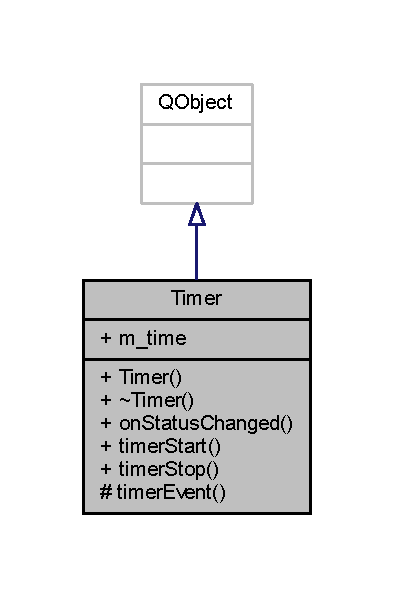
\includegraphics[width=189pt]{class_timer__inherit__graph}
\end{center}
\end{figure}


Timer 的协作图\+:
\nopagebreak
\begin{figure}[H]
\begin{center}
\leavevmode
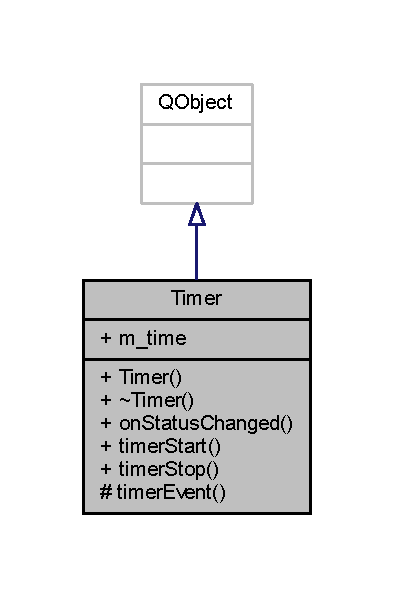
\includegraphics[width=189pt]{class_timer__coll__graph}
\end{center}
\end{figure}
\subsection*{Public 槽}
\begin{DoxyCompactItemize}
\item 
void \hyperlink{class_timer_a3dcb374fa1f7379ac2fe1130aef2b9b7}{on\+Status\+Changed} (bool s)
\item 
void \hyperlink{class_timer_a69ba0272573a9dc28b5cb48242a88fd1}{timer\+Start} ()
\item 
void \hyperlink{class_timer_adf2076ba5054ae36fc590b3d9affe6f9}{timer\+Stop} ()
\end{DoxyCompactItemize}
\subsection*{信号}
\begin{DoxyCompactItemize}
\item 
void \hyperlink{class_timer_ab8b4318d87a4ce20f552168be58dce1f}{timeout} ()
\end{DoxyCompactItemize}
\subsection*{Public 成员函数}
\begin{DoxyCompactItemize}
\item 
\hyperlink{class_timer_a32e29d892968736ffe67235892804f69}{Timer} (int interval=1000, Q\+Object $\ast$parent=0)
\item 
\hyperlink{class_timer_a14fa469c4c295c5fa6e66a4ad1092146}{$\sim$\+Timer} ()
\end{DoxyCompactItemize}
\subsection*{Public 属性}
\begin{DoxyCompactItemize}
\item 
int \hyperlink{class_timer_a89e77495174acab64a97e5aa49858cf4}{m\+\_\+time}
\end{DoxyCompactItemize}
\subsection*{Protected 成员函数}
\begin{DoxyCompactItemize}
\item 
void \hyperlink{class_timer_a45807ea29e5176d9eea65d3ee49a335a}{timer\+Event} (Q\+Timer\+Event $\ast$event)
\end{DoxyCompactItemize}


\subsection{构造及析构函数说明}
\index{Timer@{Timer}!Timer@{Timer}}
\index{Timer@{Timer}!Timer@{Timer}}
\subsubsection[{\texorpdfstring{Timer(int interval=1000, Q\+Object $\ast$parent=0)}{Timer(int interval=1000, QObject *parent=0)}}]{\setlength{\rightskip}{0pt plus 5cm}Timer\+::\+Timer (
\begin{DoxyParamCaption}
\item[{int}]{interval = {\ttfamily 1000}, }
\item[{Q\+Object $\ast$}]{parent = {\ttfamily 0}}
\end{DoxyParamCaption}
)\hspace{0.3cm}{\ttfamily [explicit]}}\hypertarget{class_timer_a32e29d892968736ffe67235892804f69}{}\label{class_timer_a32e29d892968736ffe67235892804f69}
\index{Timer@{Timer}!````~Timer@{$\sim$\+Timer}}
\index{````~Timer@{$\sim$\+Timer}!Timer@{Timer}}
\subsubsection[{\texorpdfstring{$\sim$\+Timer()}{~Timer()}}]{\setlength{\rightskip}{0pt plus 5cm}Timer\+::$\sim$\+Timer (
\begin{DoxyParamCaption}
{}
\end{DoxyParamCaption}
)}\hypertarget{class_timer_a14fa469c4c295c5fa6e66a4ad1092146}{}\label{class_timer_a14fa469c4c295c5fa6e66a4ad1092146}


\subsection{成员函数说明}
\index{Timer@{Timer}!on\+Status\+Changed@{on\+Status\+Changed}}
\index{on\+Status\+Changed@{on\+Status\+Changed}!Timer@{Timer}}
\subsubsection[{\texorpdfstring{on\+Status\+Changed}{onStatusChanged}}]{\setlength{\rightskip}{0pt plus 5cm}void Timer\+::on\+Status\+Changed (
\begin{DoxyParamCaption}
\item[{bool}]{s}
\end{DoxyParamCaption}
)\hspace{0.3cm}{\ttfamily [slot]}}\hypertarget{class_timer_a3dcb374fa1f7379ac2fe1130aef2b9b7}{}\label{class_timer_a3dcb374fa1f7379ac2fe1130aef2b9b7}
\index{Timer@{Timer}!timeout@{timeout}}
\index{timeout@{timeout}!Timer@{Timer}}
\subsubsection[{\texorpdfstring{timeout}{timeout}}]{\setlength{\rightskip}{0pt plus 5cm}void Timer\+::timeout (
\begin{DoxyParamCaption}
{}
\end{DoxyParamCaption}
)\hspace{0.3cm}{\ttfamily [signal]}}\hypertarget{class_timer_ab8b4318d87a4ce20f552168be58dce1f}{}\label{class_timer_ab8b4318d87a4ce20f552168be58dce1f}
\index{Timer@{Timer}!timer\+Event@{timer\+Event}}
\index{timer\+Event@{timer\+Event}!Timer@{Timer}}
\subsubsection[{\texorpdfstring{timer\+Event(\+Q\+Timer\+Event $\ast$event)}{timerEvent(QTimerEvent *event)}}]{\setlength{\rightskip}{0pt plus 5cm}void Timer\+::timer\+Event (
\begin{DoxyParamCaption}
\item[{Q\+Timer\+Event $\ast$}]{event}
\end{DoxyParamCaption}
)\hspace{0.3cm}{\ttfamily [protected]}}\hypertarget{class_timer_a45807ea29e5176d9eea65d3ee49a335a}{}\label{class_timer_a45807ea29e5176d9eea65d3ee49a335a}
\index{Timer@{Timer}!timer\+Start@{timer\+Start}}
\index{timer\+Start@{timer\+Start}!Timer@{Timer}}
\subsubsection[{\texorpdfstring{timer\+Start}{timerStart}}]{\setlength{\rightskip}{0pt plus 5cm}void Timer\+::timer\+Start (
\begin{DoxyParamCaption}
{}
\end{DoxyParamCaption}
)\hspace{0.3cm}{\ttfamily [slot]}}\hypertarget{class_timer_a69ba0272573a9dc28b5cb48242a88fd1}{}\label{class_timer_a69ba0272573a9dc28b5cb48242a88fd1}
\index{Timer@{Timer}!timer\+Stop@{timer\+Stop}}
\index{timer\+Stop@{timer\+Stop}!Timer@{Timer}}
\subsubsection[{\texorpdfstring{timer\+Stop}{timerStop}}]{\setlength{\rightskip}{0pt plus 5cm}void Timer\+::timer\+Stop (
\begin{DoxyParamCaption}
{}
\end{DoxyParamCaption}
)\hspace{0.3cm}{\ttfamily [slot]}}\hypertarget{class_timer_adf2076ba5054ae36fc590b3d9affe6f9}{}\label{class_timer_adf2076ba5054ae36fc590b3d9affe6f9}


\subsection{类成员变量说明}
\index{Timer@{Timer}!m\+\_\+time@{m\+\_\+time}}
\index{m\+\_\+time@{m\+\_\+time}!Timer@{Timer}}
\subsubsection[{\texorpdfstring{m\+\_\+time}{m_time}}]{\setlength{\rightskip}{0pt plus 5cm}int Timer\+::m\+\_\+time}\hypertarget{class_timer_a89e77495174acab64a97e5aa49858cf4}{}\label{class_timer_a89e77495174acab64a97e5aa49858cf4}


该类的文档由以下文件生成\+:\begin{DoxyCompactItemize}
\item 
\hyperlink{timer_8h}{timer.\+h}\item 
\hyperlink{timer_8cpp}{timer.\+cpp}\end{DoxyCompactItemize}

\chapter{文件说明}
\hypertarget{dac_8cpp}{}\section{dac.\+cpp 文件参考}
\label{dac_8cpp}\index{dac.\+cpp@{dac.\+cpp}}
{\ttfamily \#include \char`\"{}dac.\+h\char`\"{}}\\*
{\ttfamily \#include \char`\"{}daparameters.\+h\char`\"{}}\\*
{\ttfamily \#include $<$Qt\+Math$>$}\\*
dac.\+cpp 的引用(Include)关系图\+:
\nopagebreak
\begin{figure}[H]
\begin{center}
\leavevmode
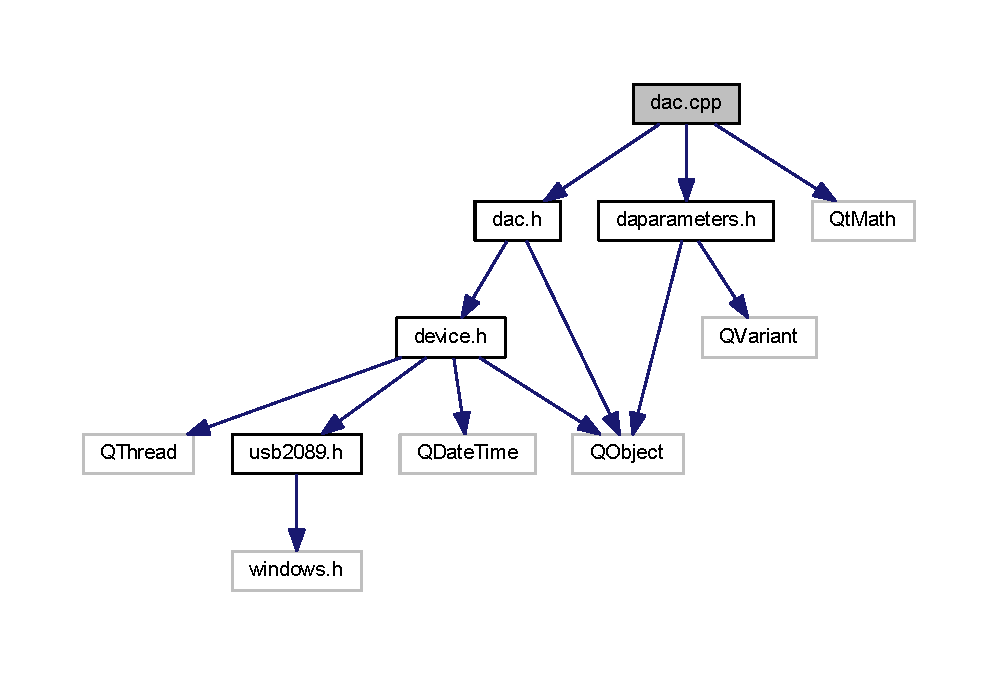
\includegraphics[width=350pt]{dac_8cpp__incl}
\end{center}
\end{figure}

\hypertarget{dac_8h}{}\section{dac.\+h 文件参考}
\label{dac_8h}\index{dac.\+h@{dac.\+h}}
{\ttfamily \#include $<$Q\+Object$>$}\\*
{\ttfamily \#include \char`\"{}device.\+h\char`\"{}}\\*
dac.\+h 的引用(Include)关系图\+:
\nopagebreak
\begin{figure}[H]
\begin{center}
\leavevmode
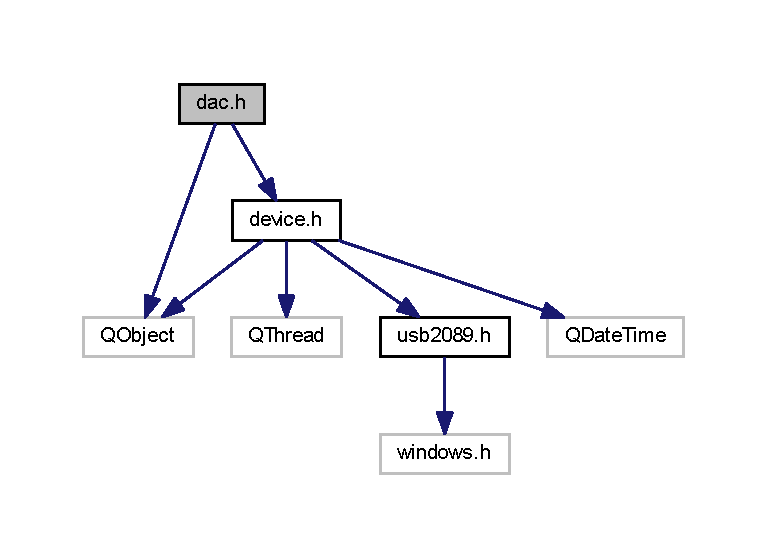
\includegraphics[width=350pt]{dac_8h__incl}
\end{center}
\end{figure}
此图展示该文件直接或间接的被哪些文件引用了\+:
\nopagebreak
\begin{figure}[H]
\begin{center}
\leavevmode
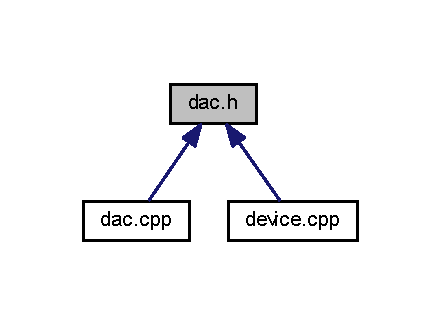
\includegraphics[width=212pt]{dac_8h__dep__incl}
\end{center}
\end{figure}
\subsection*{类}
\begin{DoxyCompactItemize}
\item 
class \hyperlink{class_d_a_c}{D\+AC}
\end{DoxyCompactItemize}
\subsection*{宏定义}
\begin{DoxyCompactItemize}
\item 
\#define \hyperlink{dac_8h_a65b26605d90a0bcd0e13e05db54f551f}{R\+ES}~25.\+0
\end{DoxyCompactItemize}


\subsection{宏定义说明}
\index{dac.\+h@{dac.\+h}!R\+ES@{R\+ES}}
\index{R\+ES@{R\+ES}!dac.\+h@{dac.\+h}}
\subsubsection[{\texorpdfstring{R\+ES}{RES}}]{\setlength{\rightskip}{0pt plus 5cm}\#define R\+ES~25.\+0}\hypertarget{dac_8h_a65b26605d90a0bcd0e13e05db54f551f}{}\label{dac_8h_a65b26605d90a0bcd0e13e05db54f551f}

\hypertarget{daparameters_8cpp}{}\section{daparameters.\+cpp 文件参考}
\label{daparameters_8cpp}\index{daparameters.\+cpp@{daparameters.\+cpp}}
{\ttfamily \#include \char`\"{}daparameters.\+h\char`\"{}}\\*
daparameters.\+cpp 的引用(Include)关系图\+:
\nopagebreak
\begin{figure}[H]
\begin{center}
\leavevmode
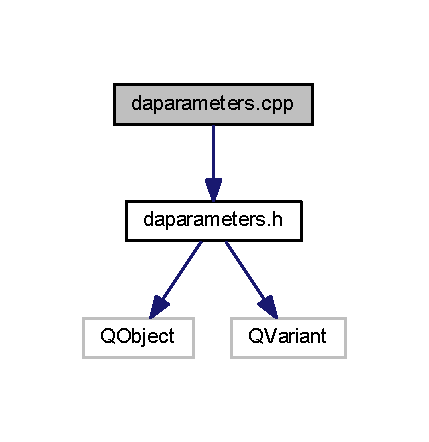
\includegraphics[width=206pt]{daparameters_8cpp__incl}
\end{center}
\end{figure}

\hypertarget{daparameters_8h}{}\section{daparameters.\+h 文件参考}
\label{daparameters_8h}\index{daparameters.\+h@{daparameters.\+h}}
{\ttfamily \#include $<$Q\+Object$>$}\\*
{\ttfamily \#include $<$Q\+Variant$>$}\\*
daparameters.\+h 的引用(Include)关系图\+:
\nopagebreak
\begin{figure}[H]
\begin{center}
\leavevmode
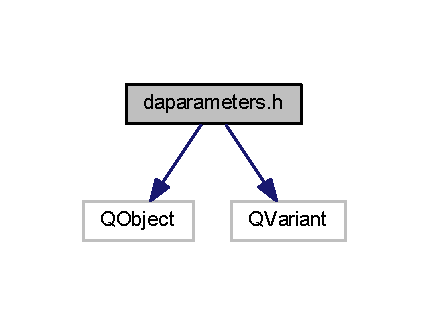
\includegraphics[width=206pt]{daparameters_8h__incl}
\end{center}
\end{figure}
此图展示该文件直接或间接的被哪些文件引用了\+:
\nopagebreak
\begin{figure}[H]
\begin{center}
\leavevmode
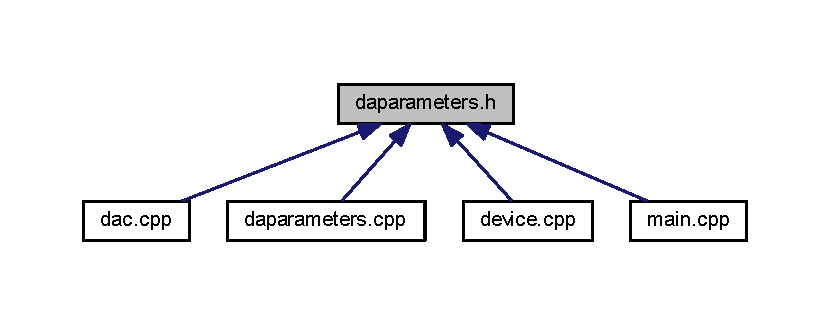
\includegraphics[width=350pt]{daparameters_8h__dep__incl}
\end{center}
\end{figure}
\subsection*{类}
\begin{DoxyCompactItemize}
\item 
class \hyperlink{class_d_a_parameters}{D\+A\+Parameters}
\end{DoxyCompactItemize}
\subsection*{宏定义}
\begin{DoxyCompactItemize}
\item 
\#define \hyperlink{daparameters_8h_a8c6378801cd6a711ec34d75a857cb77d}{D\+A\+C\+H\+A\+N\+N\+EL}~12
\end{DoxyCompactItemize}


\subsection{宏定义说明}
\index{daparameters.\+h@{daparameters.\+h}!D\+A\+C\+H\+A\+N\+N\+EL@{D\+A\+C\+H\+A\+N\+N\+EL}}
\index{D\+A\+C\+H\+A\+N\+N\+EL@{D\+A\+C\+H\+A\+N\+N\+EL}!daparameters.\+h@{daparameters.\+h}}
\subsubsection[{\texorpdfstring{D\+A\+C\+H\+A\+N\+N\+EL}{DACHANNEL}}]{\setlength{\rightskip}{0pt plus 5cm}\#define D\+A\+C\+H\+A\+N\+N\+EL~12}\hypertarget{daparameters_8h_a8c6378801cd6a711ec34d75a857cb77d}{}\label{daparameters_8h_a8c6378801cd6a711ec34d75a857cb77d}

\hypertarget{daq_8cpp}{}\section{daq.\+cpp 文件参考}
\label{daq_8cpp}\index{daq.\+cpp@{daq.\+cpp}}
{\ttfamily \#include \char`\"{}daq.\+h\char`\"{}}\\*
{\ttfamily \#include $<$Q\+Date\+Time$>$}\\*
daq.\+cpp 的引用(Include)关系图\+:
\nopagebreak
\begin{figure}[H]
\begin{center}
\leavevmode
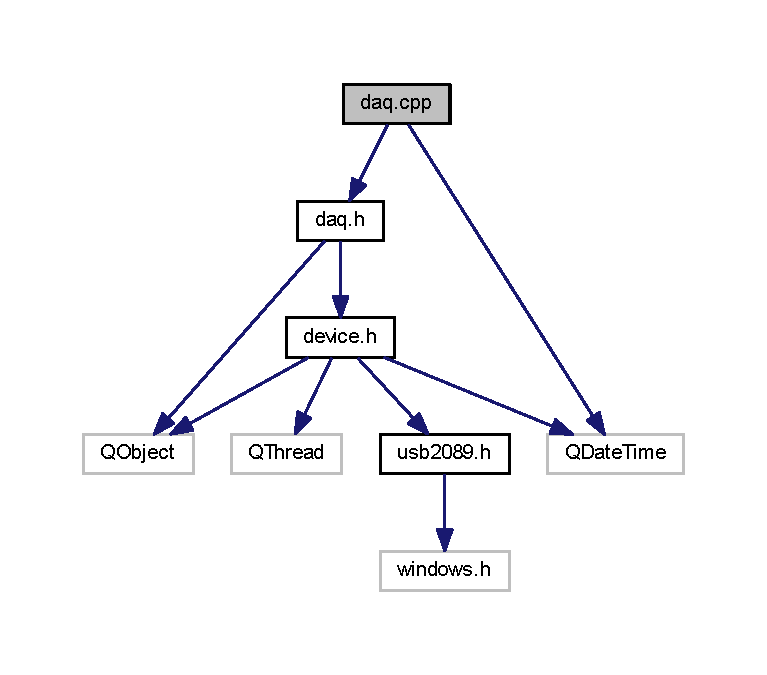
\includegraphics[width=350pt]{daq_8cpp__incl}
\end{center}
\end{figure}

\hypertarget{daq_8h}{}\section{daq.\+h 文件参考}
\label{daq_8h}\index{daq.\+h@{daq.\+h}}
{\ttfamily \#include $<$Q\+Object$>$}\\*
{\ttfamily \#include \char`\"{}device.\+h\char`\"{}}\\*
daq.\+h 的引用(Include)关系图\+:
\nopagebreak
\begin{figure}[H]
\begin{center}
\leavevmode
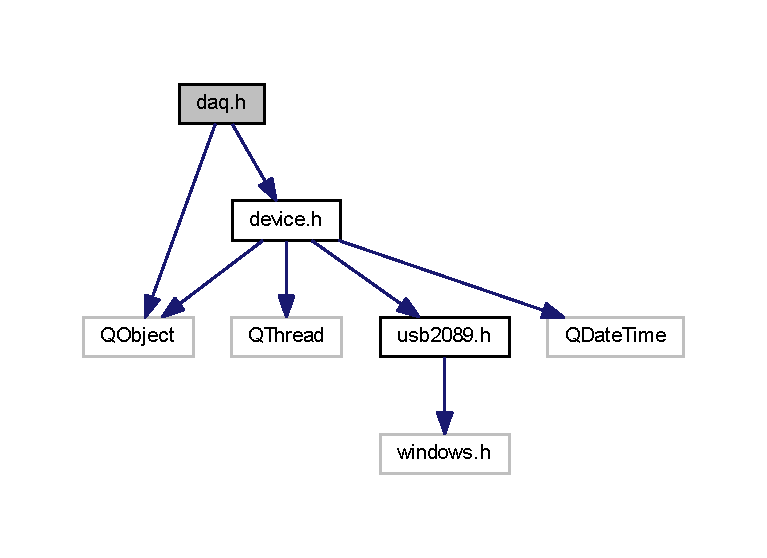
\includegraphics[width=350pt]{daq_8h__incl}
\end{center}
\end{figure}
此图展示该文件直接或间接的被哪些文件引用了\+:
\nopagebreak
\begin{figure}[H]
\begin{center}
\leavevmode
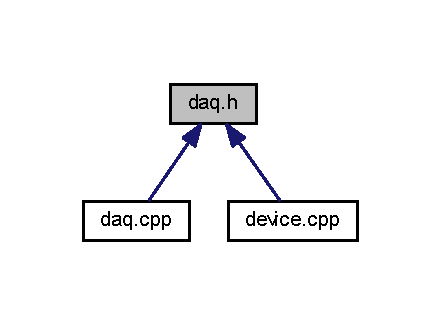
\includegraphics[width=212pt]{daq_8h__dep__incl}
\end{center}
\end{figure}
\subsection*{类}
\begin{DoxyCompactItemize}
\item 
class \hyperlink{class_d_a_q}{D\+AQ}
\end{DoxyCompactItemize}

\hypertarget{database_8cpp}{}\section{database.\+cpp 文件参考}
\label{database_8cpp}\index{database.\+cpp@{database.\+cpp}}
{\ttfamily \#include \char`\"{}database.\+h\char`\"{}}\\*
{\ttfamily \#include $<$Q\+Sql\+Database$>$}\\*
{\ttfamily \#include $<$Q\+Sql\+Query$>$}\\*
{\ttfamily \#include $<$Q\+Thread$>$}\\*
{\ttfamily \#include $<$Q\+Reg\+Exp$>$}\\*
{\ttfamily \#include $<$Qt\+Xlsx$>$}\\*
database.\+cpp 的引用(Include)关系图\+:
\nopagebreak
\begin{figure}[H]
\begin{center}
\leavevmode
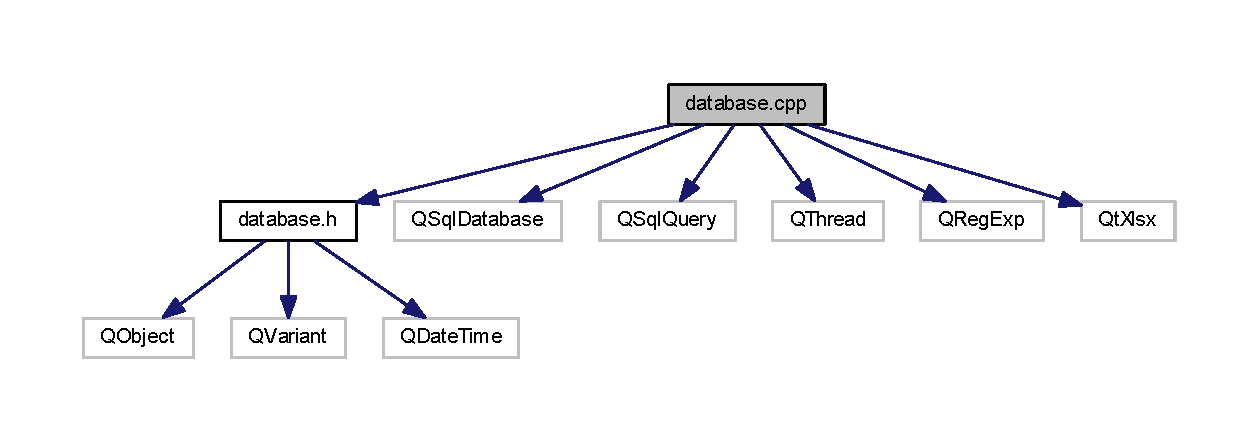
\includegraphics[width=350pt]{database_8cpp__incl}
\end{center}
\end{figure}

\hypertarget{database_8h}{}\section{database.\+h 文件参考}
\label{database_8h}\index{database.\+h@{database.\+h}}
{\ttfamily \#include $<$Q\+Object$>$}\\*
{\ttfamily \#include $<$Q\+Variant$>$}\\*
{\ttfamily \#include $<$Q\+Date\+Time$>$}\\*
database.\+h 的引用(Include)关系图\+:
\nopagebreak
\begin{figure}[H]
\begin{center}
\leavevmode
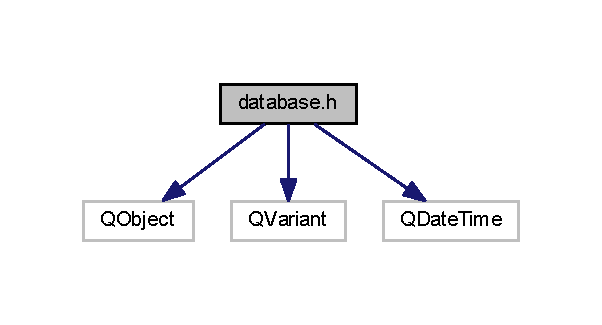
\includegraphics[width=289pt]{database_8h__incl}
\end{center}
\end{figure}
此图展示该文件直接或间接的被哪些文件引用了\+:
\nopagebreak
\begin{figure}[H]
\begin{center}
\leavevmode
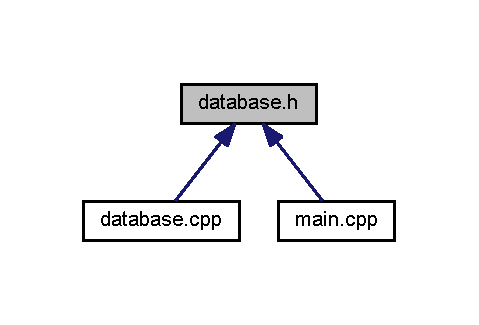
\includegraphics[width=230pt]{database_8h__dep__incl}
\end{center}
\end{figure}
\subsection*{类}
\begin{DoxyCompactItemize}
\item 
class \hyperlink{class_d_b_worker}{D\+B\+Worker}
\item 
class \hyperlink{class_database}{Database}
\end{DoxyCompactItemize}

\hypertarget{datasource_8cpp}{}\section{datasource.\+cpp 文件参考}
\label{datasource_8cpp}\index{datasource.\+cpp@{datasource.\+cpp}}
{\ttfamily \#include \char`\"{}datasource.\+h\char`\"{}}\\*
{\ttfamily \#include \char`\"{}device.\+h\char`\"{}}\\*
{\ttfamily \#include $<$Qt\+Charts/\+Q\+X\+Y\+Series$>$}\\*
{\ttfamily \#include $<$Qt\+Charts/\+Q\+Area\+Series$>$}\\*
{\ttfamily \#include $<$Qt\+Quick/\+Q\+Quick\+View$>$}\\*
{\ttfamily \#include $<$Qt\+Quick/\+Q\+Quick\+Item$>$}\\*
{\ttfamily \#include $<$Qt\+Core/\+Q\+Debug$>$}\\*
{\ttfamily \#include $<$Qt\+Core/\+Qt\+Math$>$}\\*
{\ttfamily \#include $<$Qt\+Global$>$}\\*
datasource.\+cpp 的引用(Include)关系图\+:
\nopagebreak
\begin{figure}[H]
\begin{center}
\leavevmode
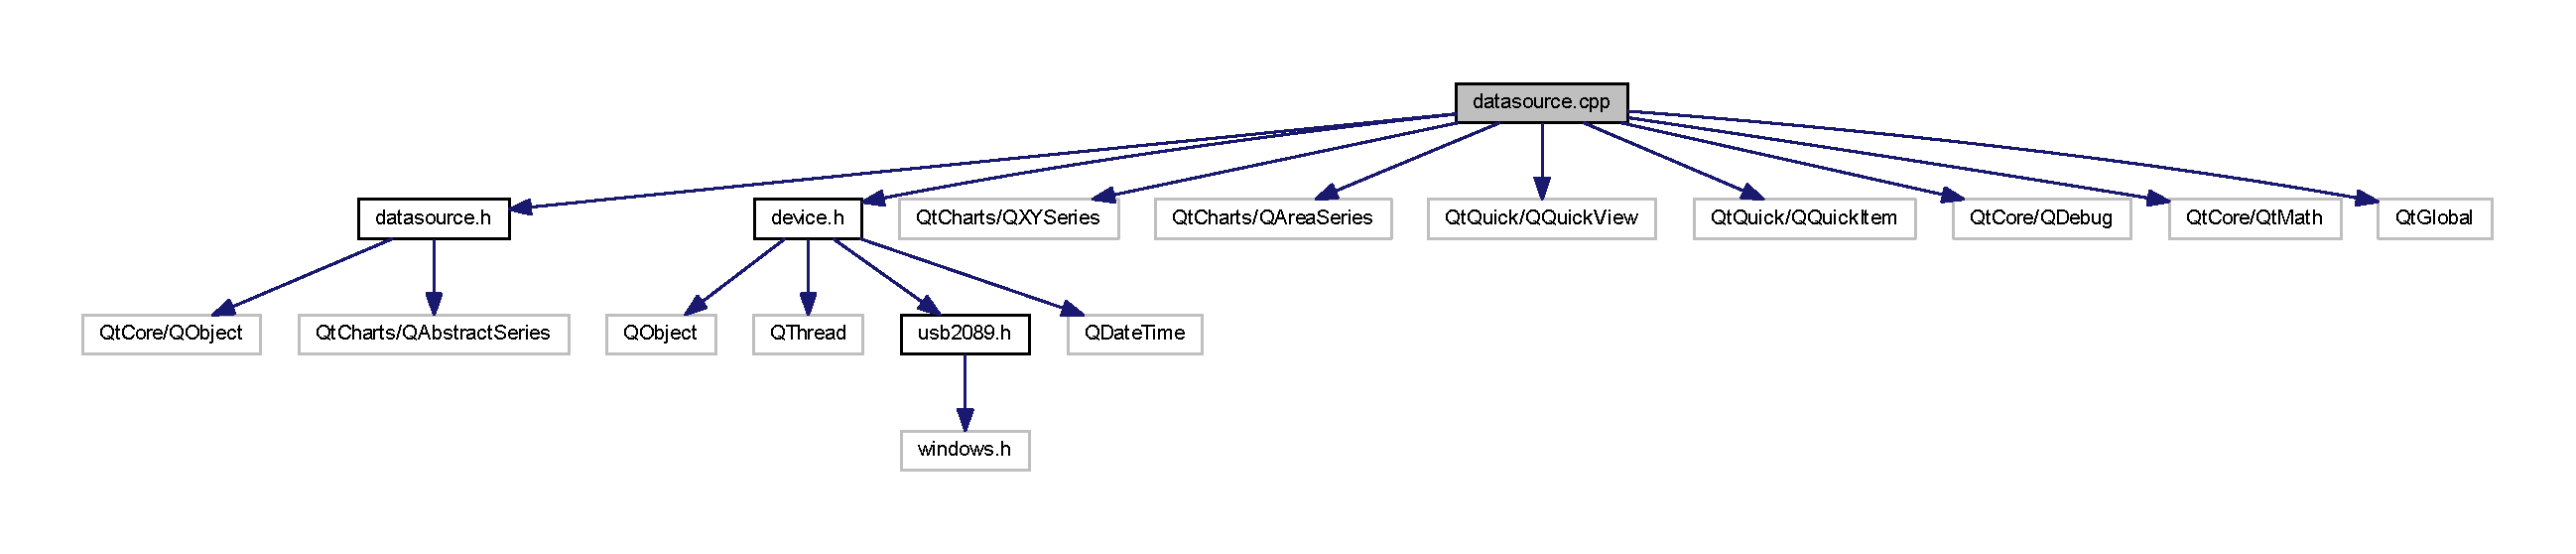
\includegraphics[width=350pt]{datasource_8cpp__incl}
\end{center}
\end{figure}

\hypertarget{datasource_8h}{}\section{datasource.\+h 文件参考}
\label{datasource_8h}\index{datasource.\+h@{datasource.\+h}}
{\ttfamily \#include $<$Qt\+Core/\+Q\+Object$>$}\\*
{\ttfamily \#include $<$Qt\+Charts/\+Q\+Abstract\+Series$>$}\\*
datasource.\+h 的引用(Include)关系图\+:
\nopagebreak
\begin{figure}[H]
\begin{center}
\leavevmode
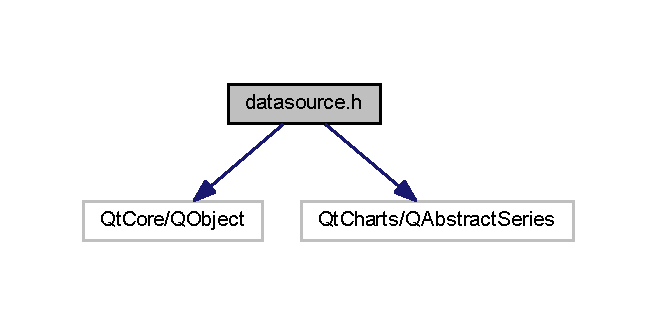
\includegraphics[width=316pt]{datasource_8h__incl}
\end{center}
\end{figure}
此图展示该文件直接或间接的被哪些文件引用了\+:
\nopagebreak
\begin{figure}[H]
\begin{center}
\leavevmode
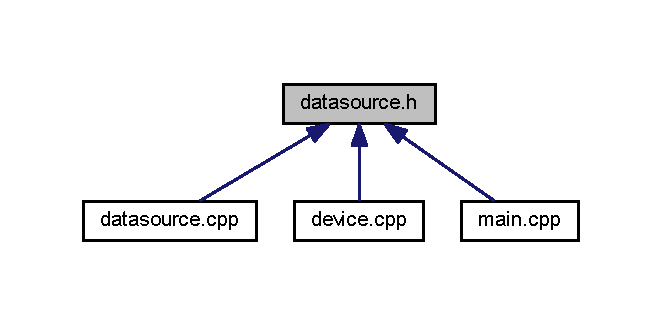
\includegraphics[width=318pt]{datasource_8h__dep__incl}
\end{center}
\end{figure}
\subsection*{类}
\begin{DoxyCompactItemize}
\item 
class \hyperlink{class_data_source}{Data\+Source}
\end{DoxyCompactItemize}

\hypertarget{device_8cpp}{}\section{device.\+cpp 文件参考}
\label{device_8cpp}\index{device.\+cpp@{device.\+cpp}}
{\ttfamily \#include \char`\"{}device.\+h\char`\"{}}\\*
{\ttfamily \#include \char`\"{}serial.\+h\char`\"{}}\\*
{\ttfamily \#include \char`\"{}daq.\+h\char`\"{}}\\*
{\ttfamily \#include \char`\"{}dac.\+h\char`\"{}}\\*
{\ttfamily \#include \char`\"{}gasdata.\+h\char`\"{}}\\*
{\ttfamily \#include \char`\"{}daparameters.\+h\char`\"{}}\\*
{\ttfamily \#include \char`\"{}datasource.\+h\char`\"{}}\\*
{\ttfamily \#include \char`\"{}timer.\+h\char`\"{}}\\*
device.\+cpp 的引用(Include)关系图\+:
\nopagebreak
\begin{figure}[H]
\begin{center}
\leavevmode
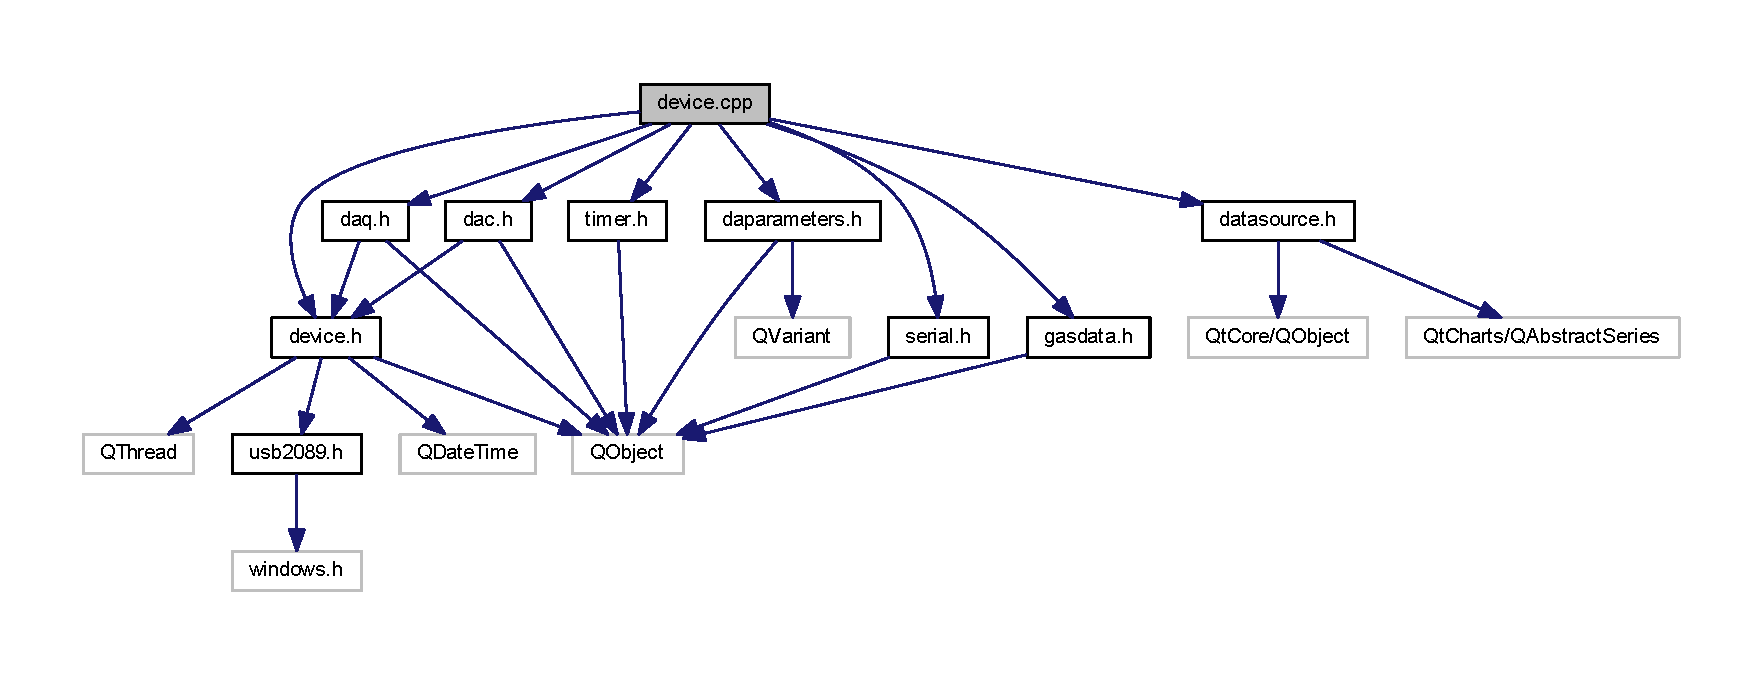
\includegraphics[width=350pt]{device_8cpp__incl}
\end{center}
\end{figure}

\hypertarget{device_8h}{}\section{device.\+h 文件参考}
\label{device_8h}\index{device.\+h@{device.\+h}}
{\ttfamily \#include $<$Q\+Object$>$}\\*
{\ttfamily \#include $<$Q\+Thread$>$}\\*
{\ttfamily \#include \char`\"{}usb2089.\+h\char`\"{}}\\*
{\ttfamily \#include $<$Q\+Date\+Time$>$}\\*
device.\+h 的引用(Include)关系图\+:
\nopagebreak
\begin{figure}[H]
\begin{center}
\leavevmode
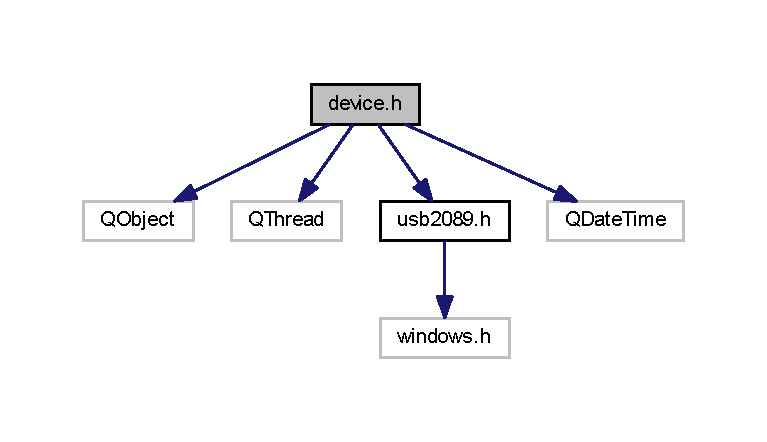
\includegraphics[width=350pt]{device_8h__incl}
\end{center}
\end{figure}
此图展示该文件直接或间接的被哪些文件引用了\+:
\nopagebreak
\begin{figure}[H]
\begin{center}
\leavevmode
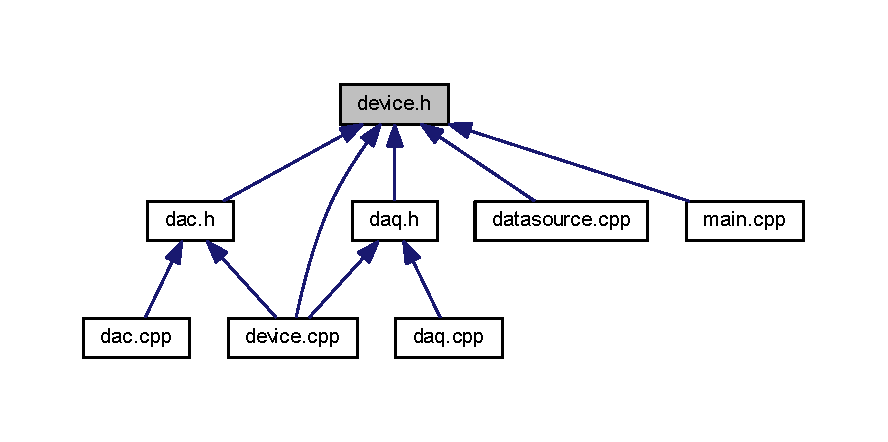
\includegraphics[width=350pt]{device_8h__dep__incl}
\end{center}
\end{figure}
\subsection*{类}
\begin{DoxyCompactItemize}
\item 
class \hyperlink{class_device}{Device}
\end{DoxyCompactItemize}
\subsection*{宏定义}
\begin{DoxyCompactItemize}
\item 
\#define \hyperlink{device_8h_a3dc717773b96807e0f47b500b2f7ac04}{D\+E\+V\+C\+NT}~2
\item 
\#define \hyperlink{device_8h_aa58e0287a2b6f1815a98c7e5e6724e20}{D\+E\+V\+ID}~0
\end{DoxyCompactItemize}


\subsection{宏定义说明}
\index{device.\+h@{device.\+h}!D\+E\+V\+C\+NT@{D\+E\+V\+C\+NT}}
\index{D\+E\+V\+C\+NT@{D\+E\+V\+C\+NT}!device.\+h@{device.\+h}}
\subsubsection[{\texorpdfstring{D\+E\+V\+C\+NT}{DEVCNT}}]{\setlength{\rightskip}{0pt plus 5cm}\#define D\+E\+V\+C\+NT~2}\hypertarget{device_8h_a3dc717773b96807e0f47b500b2f7ac04}{}\label{device_8h_a3dc717773b96807e0f47b500b2f7ac04}
\index{device.\+h@{device.\+h}!D\+E\+V\+ID@{D\+E\+V\+ID}}
\index{D\+E\+V\+ID@{D\+E\+V\+ID}!device.\+h@{device.\+h}}
\subsubsection[{\texorpdfstring{D\+E\+V\+ID}{DEVID}}]{\setlength{\rightskip}{0pt plus 5cm}\#define D\+E\+V\+ID~0}\hypertarget{device_8h_aa58e0287a2b6f1815a98c7e5e6724e20}{}\label{device_8h_aa58e0287a2b6f1815a98c7e5e6724e20}

\hypertarget{gasdata_8cpp}{}\section{gasdata.\+cpp 文件参考}
\label{gasdata_8cpp}\index{gasdata.\+cpp@{gasdata.\+cpp}}
{\ttfamily \#include \char`\"{}gasdata.\+h\char`\"{}}\\*
{\ttfamily \#include $<$Q\+Date\+Time$>$}\\*
gasdata.\+cpp 的引用(Include)关系图\+:
\nopagebreak
\begin{figure}[H]
\begin{center}
\leavevmode
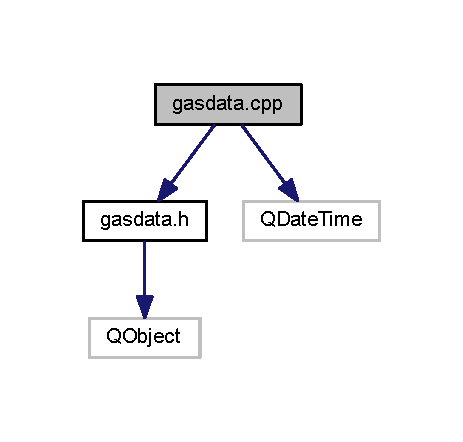
\includegraphics[width=222pt]{gasdata_8cpp__incl}
\end{center}
\end{figure}

\hypertarget{gasdata_8h}{}\section{gasdata.\+h 文件参考}
\label{gasdata_8h}\index{gasdata.\+h@{gasdata.\+h}}
{\ttfamily \#include $<$Q\+Object$>$}\\*
gasdata.\+h 的引用(Include)关系图\+:
\nopagebreak
\begin{figure}[H]
\begin{center}
\leavevmode
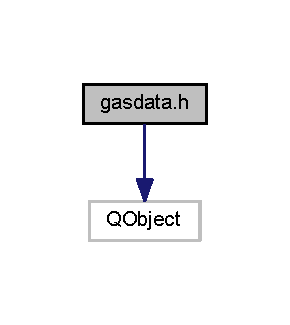
\includegraphics[width=139pt]{gasdata_8h__incl}
\end{center}
\end{figure}
此图展示该文件直接或间接的被哪些文件引用了\+:
\nopagebreak
\begin{figure}[H]
\begin{center}
\leavevmode
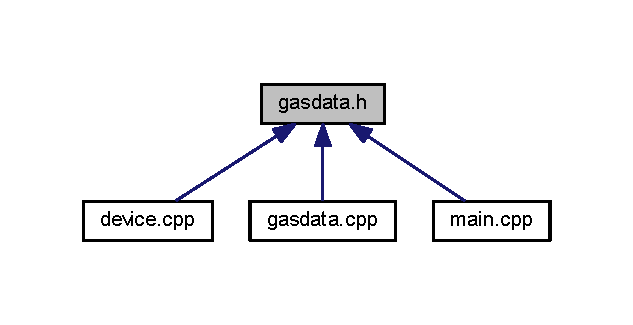
\includegraphics[width=304pt]{gasdata_8h__dep__incl}
\end{center}
\end{figure}
\subsection*{类}
\begin{DoxyCompactItemize}
\item 
class \hyperlink{class_gas_data}{Gas\+Data}
\end{DoxyCompactItemize}

\hypertarget{main_8cpp}{}\section{main.\+cpp 文件参考}
\label{main_8cpp}\index{main.\+cpp@{main.\+cpp}}
{\ttfamily \#include $<$Q\+Application$>$}\\*
{\ttfamily \#include $<$Q\+Qml\+Application\+Engine$>$}\\*
{\ttfamily \#include $<$Q\+Thread$>$}\\*
{\ttfamily \#include $<$Qt\+Web\+Engine$>$}\\*
{\ttfamily \#include $<$Qt\+Qml$>$}\\*
{\ttfamily \#include \char`\"{}device.\+h\char`\"{}}\\*
{\ttfamily \#include \char`\"{}gasdata.\+h\char`\"{}}\\*
{\ttfamily \#include \char`\"{}daparameters.\+h\char`\"{}}\\*
{\ttfamily \#include \char`\"{}datasource.\+h\char`\"{}}\\*
{\ttfamily \#include \char`\"{}database.\+h\char`\"{}}\\*
{\ttfamily \#include $<$Q\+Data\+Stream$>$}\\*
main.\+cpp 的引用(Include)关系图\+:
\nopagebreak
\begin{figure}[H]
\begin{center}
\leavevmode
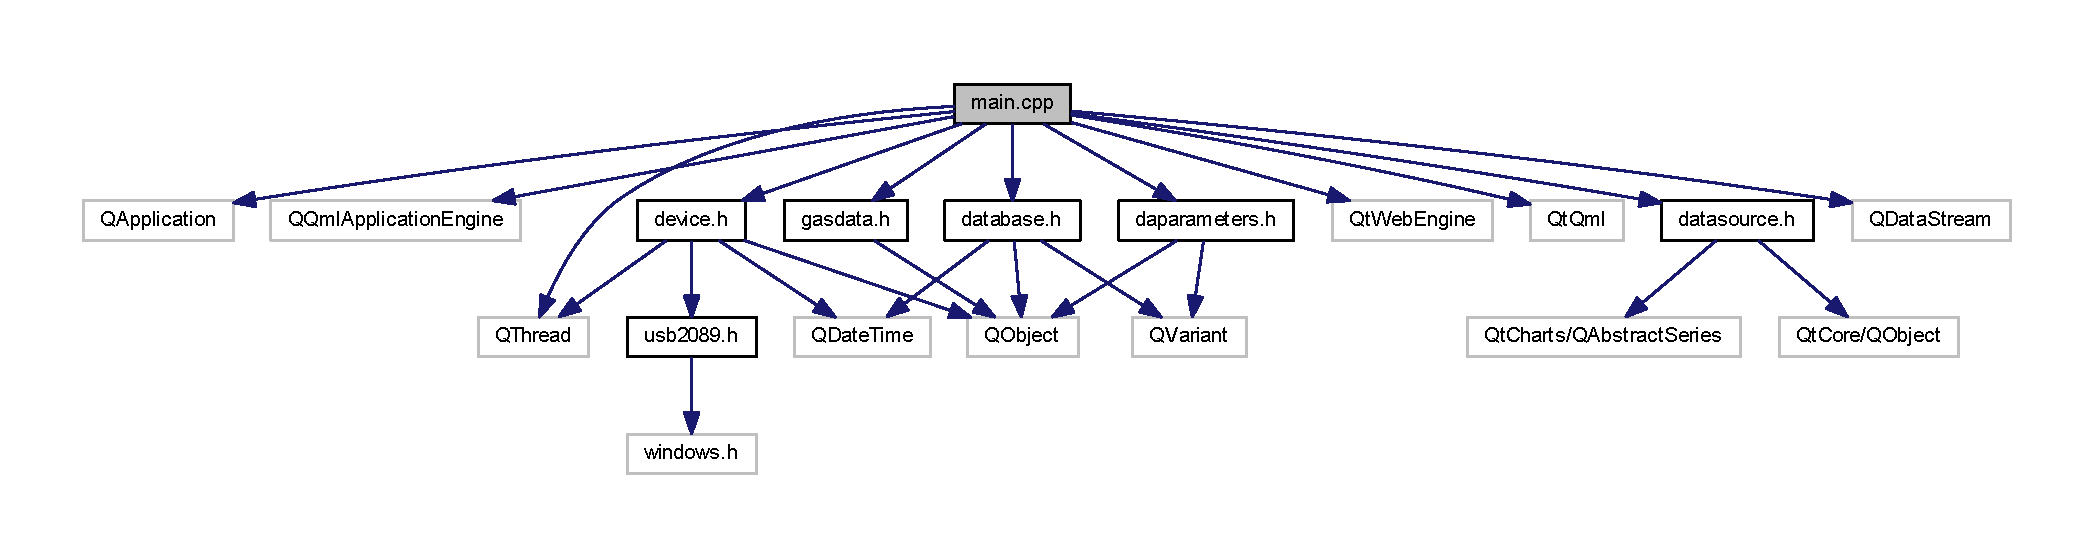
\includegraphics[width=350pt]{main_8cpp__incl}
\end{center}
\end{figure}
\subsection*{函数}
\begin{DoxyCompactItemize}
\item 
int \hyperlink{main_8cpp_a3c04138a5bfe5d72780bb7e82a18e627}{main} (int argc, char $\ast$$\ast$argv)
\end{DoxyCompactItemize}
\subsection*{变量}
\begin{DoxyCompactItemize}
\item 
qint16 \hyperlink{main_8cpp_a13b8719ad4f98332b84f4dc6f3ef447c}{ad\+Buffer} \mbox{[}1024\mbox{]}
\end{DoxyCompactItemize}


\subsection{函数说明}
\index{main.\+cpp@{main.\+cpp}!main@{main}}
\index{main@{main}!main.\+cpp@{main.\+cpp}}
\subsubsection[{\texorpdfstring{main(int argc, char $\ast$$\ast$argv)}{main(int argc, char **argv)}}]{\setlength{\rightskip}{0pt plus 5cm}int main (
\begin{DoxyParamCaption}
\item[{int}]{argc, }
\item[{char $\ast$$\ast$}]{argv}
\end{DoxyParamCaption}
)}\hypertarget{main_8cpp_a3c04138a5bfe5d72780bb7e82a18e627}{}\label{main_8cpp_a3c04138a5bfe5d72780bb7e82a18e627}


\subsection{变量说明}
\index{main.\+cpp@{main.\+cpp}!ad\+Buffer@{ad\+Buffer}}
\index{ad\+Buffer@{ad\+Buffer}!main.\+cpp@{main.\+cpp}}
\subsubsection[{\texorpdfstring{ad\+Buffer}{adBuffer}}]{\setlength{\rightskip}{0pt plus 5cm}qint16 ad\+Buffer\mbox{[}1024\mbox{]}}\hypertarget{main_8cpp_a13b8719ad4f98332b84f4dc6f3ef447c}{}\label{main_8cpp_a13b8719ad4f98332b84f4dc6f3ef447c}

\hypertarget{serial_8cpp}{}\section{serial.\+cpp 文件参考}
\label{serial_8cpp}\index{serial.\+cpp@{serial.\+cpp}}
{\ttfamily \#include \char`\"{}serial.\+h\char`\"{}}\\*
{\ttfamily \#include $<$Q\+Serial\+Port$>$}\\*
{\ttfamily \#include $<$Q\+Data\+Stream$>$}\\*
serial.\+cpp 的引用(Include)关系图\+:
\nopagebreak
\begin{figure}[H]
\begin{center}
\leavevmode
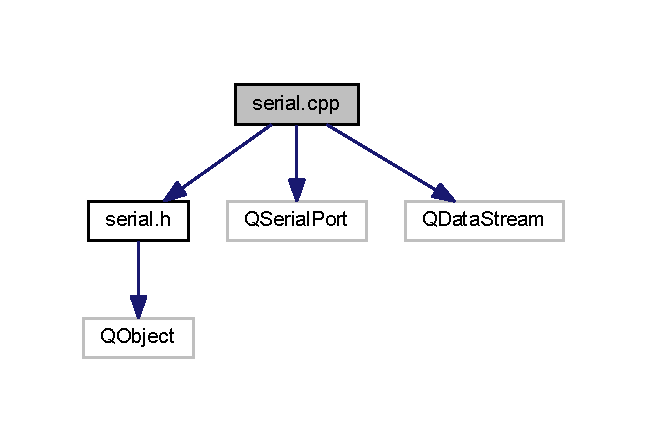
\includegraphics[width=311pt]{serial_8cpp__incl}
\end{center}
\end{figure}

\hypertarget{serial_8h}{}\section{serial.\+h 文件参考}
\label{serial_8h}\index{serial.\+h@{serial.\+h}}
{\ttfamily \#include $<$Q\+Object$>$}\\*
serial.\+h 的引用(Include)关系图\+:
\nopagebreak
\begin{figure}[H]
\begin{center}
\leavevmode
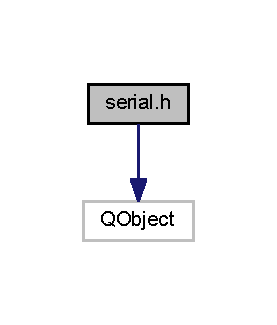
\includegraphics[width=133pt]{serial_8h__incl}
\end{center}
\end{figure}
此图展示该文件直接或间接的被哪些文件引用了\+:
\nopagebreak
\begin{figure}[H]
\begin{center}
\leavevmode
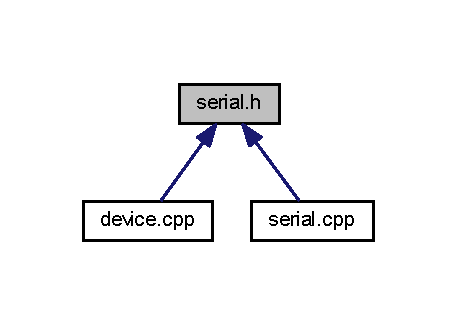
\includegraphics[width=220pt]{serial_8h__dep__incl}
\end{center}
\end{figure}
\subsection*{类}
\begin{DoxyCompactItemize}
\item 
class \hyperlink{class_serial}{Serial}
\end{DoxyCompactItemize}
\subsection*{宏定义}
\begin{DoxyCompactItemize}
\item 
\#define \hyperlink{serial_8h_ac0beba2a174e40134363704220906af7}{P\+O\+R\+T\+N\+A\+ME}~\char`\"{}C\+O\+M3\char`\"{}
\end{DoxyCompactItemize}


\subsection{宏定义说明}
\index{serial.\+h@{serial.\+h}!P\+O\+R\+T\+N\+A\+ME@{P\+O\+R\+T\+N\+A\+ME}}
\index{P\+O\+R\+T\+N\+A\+ME@{P\+O\+R\+T\+N\+A\+ME}!serial.\+h@{serial.\+h}}
\subsubsection[{\texorpdfstring{P\+O\+R\+T\+N\+A\+ME}{PORTNAME}}]{\setlength{\rightskip}{0pt plus 5cm}\#define P\+O\+R\+T\+N\+A\+ME~\char`\"{}C\+O\+M3\char`\"{}}\hypertarget{serial_8h_ac0beba2a174e40134363704220906af7}{}\label{serial_8h_ac0beba2a174e40134363704220906af7}

\hypertarget{timer_8cpp}{}\section{timer.\+cpp 文件参考}
\label{timer_8cpp}\index{timer.\+cpp@{timer.\+cpp}}
{\ttfamily \#include \char`\"{}timer.\+h\char`\"{}}\\*
timer.\+cpp 的引用(Include)关系图\+:
\nopagebreak
\begin{figure}[H]
\begin{center}
\leavevmode
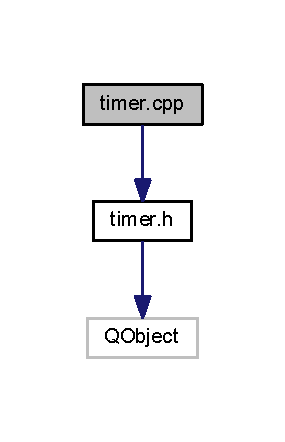
\includegraphics[width=137pt]{timer_8cpp__incl}
\end{center}
\end{figure}

\hypertarget{timer_8h}{}\section{timer.\+h 文件参考}
\label{timer_8h}\index{timer.\+h@{timer.\+h}}
{\ttfamily \#include $<$Q\+Object$>$}\\*
timer.\+h 的引用(Include)关系图\+:
\nopagebreak
\begin{figure}[H]
\begin{center}
\leavevmode
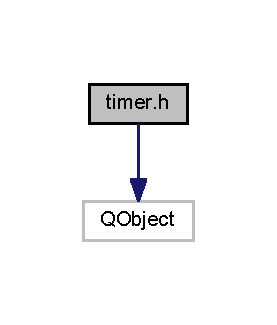
\includegraphics[width=133pt]{timer_8h__incl}
\end{center}
\end{figure}
此图展示该文件直接或间接的被哪些文件引用了\+:
\nopagebreak
\begin{figure}[H]
\begin{center}
\leavevmode
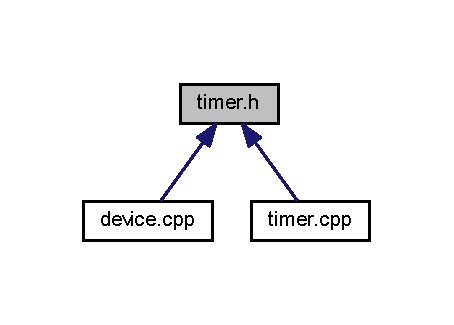
\includegraphics[width=218pt]{timer_8h__dep__incl}
\end{center}
\end{figure}
\subsection*{类}
\begin{DoxyCompactItemize}
\item 
class \hyperlink{class_timer}{Timer}
\end{DoxyCompactItemize}

\hypertarget{usb2089_8h}{}\section{usb2089.\+h 文件参考}
\label{usb2089_8h}\index{usb2089.\+h@{usb2089.\+h}}
{\ttfamily \#include $<$windows.\+h$>$}\\*
usb2089.\+h 的引用(Include)关系图\+:
\nopagebreak
\begin{figure}[H]
\begin{center}
\leavevmode
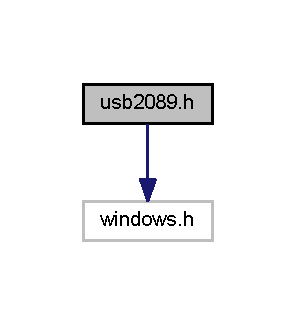
\includegraphics[width=142pt]{usb2089_8h__incl}
\end{center}
\end{figure}
此图展示该文件直接或间接的被哪些文件引用了\+:
\nopagebreak
\begin{figure}[H]
\begin{center}
\leavevmode
\includegraphics[width=350pt]{usb2089_8h__dep__incl}
\end{center}
\end{figure}
\subsection*{类}
\begin{DoxyCompactItemize}
\item 
struct \hyperlink{struct___u_s_b2089___p_a_r_a___a_d}{\+\_\+\+U\+S\+B2089\+\_\+\+P\+A\+R\+A\+\_\+\+AD}
\end{DoxyCompactItemize}
\subsection*{宏定义}
\begin{DoxyCompactItemize}
\item 
\#define \hyperlink{usb2089_8h_a7bcd7cf37ca113cfc3b43f879e86b2c4}{D\+E\+V\+A\+PI}~\+\_\+\+\_\+declspec(dllimport)
\end{DoxyCompactItemize}
\subsection*{类型定义}
\begin{DoxyCompactItemize}
\item 
typedef struct \hyperlink{struct___u_s_b2089___p_a_r_a___a_d}{\+\_\+\+U\+S\+B2089\+\_\+\+P\+A\+R\+A\+\_\+\+AD} \hyperlink{usb2089_8h_a7e2242389eec239fbf45ae3dd7ba053f}{U\+S\+B2089\+\_\+\+P\+A\+R\+A\+\_\+\+AD}
\item 
typedef struct \hyperlink{struct___u_s_b2089___p_a_r_a___a_d}{\+\_\+\+U\+S\+B2089\+\_\+\+P\+A\+R\+A\+\_\+\+AD} $\ast$ \hyperlink{usb2089_8h_a0d5fb97ed329abb3e67f76c2bd4959db}{P\+U\+S\+B2089\+\_\+\+P\+A\+R\+A\+\_\+\+AD}
\end{DoxyCompactItemize}
\subsection*{函数}
\begin{DoxyCompactItemize}
\item 
H\+A\+N\+D\+LE \hyperlink{usb2089_8h_a7bcd7cf37ca113cfc3b43f879e86b2c4}{D\+E\+V\+A\+PI} F\+AR P\+A\+S\+C\+AL \hyperlink{usb2089_8h_acf1e685b4881d03a964da49293c1df7e}{U\+S\+B2089\+\_\+\+Create\+Device} (int Device\+Lgc\+ID=0)
\item 
int \hyperlink{usb2089_8h_a7bcd7cf37ca113cfc3b43f879e86b2c4}{D\+E\+V\+A\+PI} F\+AR P\+A\+S\+C\+AL \hyperlink{usb2089_8h_ae080cea798e33b1d405b6a7d827d9006}{U\+S\+B2089\+\_\+\+Get\+Device\+Count} (H\+A\+N\+D\+LE h\+Device)
\item 
int \hyperlink{usb2089_8h_a7bcd7cf37ca113cfc3b43f879e86b2c4}{D\+E\+V\+A\+PI} F\+AR P\+A\+S\+C\+AL \hyperlink{usb2089_8h_a68e7fc40f04d78bfcbaf7136906923dc}{U\+S\+B2089\+\_\+\+Get\+Device\+Current\+ID} (H\+A\+N\+D\+LE h\+Device)
\item 
B\+O\+OL \hyperlink{usb2089_8h_a7bcd7cf37ca113cfc3b43f879e86b2c4}{D\+E\+V\+A\+PI} F\+AR P\+A\+S\+C\+AL \hyperlink{usb2089_8h_a5496561d622cf0e39812db7943c4d099}{U\+S\+B2089\+\_\+\+Reset\+Device} (H\+A\+N\+D\+LE h\+Device)
\item 
B\+O\+OL \hyperlink{usb2089_8h_a7bcd7cf37ca113cfc3b43f879e86b2c4}{D\+E\+V\+A\+PI} F\+AR P\+A\+S\+C\+AL \hyperlink{usb2089_8h_abea9e1fa8752ac5d5610166ee6126410}{U\+S\+B2089\+\_\+\+Release\+Device} (H\+A\+N\+D\+LE h\+Device)
\item 
B\+O\+OL \hyperlink{usb2089_8h_a7bcd7cf37ca113cfc3b43f879e86b2c4}{D\+E\+V\+A\+PI} F\+AR P\+A\+S\+C\+AL \hyperlink{usb2089_8h_aaa49b744edb67627cdeb6fb801c2595d}{U\+S\+B2089\+\_\+\+Init\+Device\+AD} (H\+A\+N\+D\+LE h\+Device, \hyperlink{usb2089_8h_a0d5fb97ed329abb3e67f76c2bd4959db}{P\+U\+S\+B2089\+\_\+\+P\+A\+R\+A\+\_\+\+AD} p\+A\+D\+Para)
\item 
B\+O\+OL \hyperlink{usb2089_8h_a7bcd7cf37ca113cfc3b43f879e86b2c4}{D\+E\+V\+A\+PI} F\+AR P\+A\+S\+C\+AL \hyperlink{usb2089_8h_ad2c27d25698ee42a25bba14b39f86ab9}{U\+S\+B2089\+\_\+\+Get\+Device\+Status\+AD} (H\+A\+N\+D\+LE h\+Device, P\+B\+O\+OL b\+Trig\+Flag, P\+B\+O\+OL b\+Converting, P\+B\+O\+OL b\+Overflow)
\item 
B\+O\+OL \hyperlink{usb2089_8h_a7bcd7cf37ca113cfc3b43f879e86b2c4}{D\+E\+V\+A\+PI} F\+AR P\+A\+S\+C\+AL \hyperlink{usb2089_8h_adb553543228544d7b025ba8f16b3efec}{U\+S\+B2089\+\_\+\+Read\+Device\+AD} (H\+A\+N\+D\+LE h\+Device, S\+H\+O\+RT A\+D\+Buffer\mbox{[}$\,$\mbox{]}, L\+O\+NG n\+Read\+Size\+Words, P\+L\+O\+NG n\+Ret\+Size\+Words)
\item 
B\+O\+OL \hyperlink{usb2089_8h_a7bcd7cf37ca113cfc3b43f879e86b2c4}{D\+E\+V\+A\+PI} F\+AR P\+A\+S\+C\+AL \hyperlink{usb2089_8h_afda0ec85a5685813dd19e4e30b3cf050}{U\+S\+B2089\+\_\+\+Release\+Device\+AD} (H\+A\+N\+D\+LE h\+Device)
\item 
B\+O\+OL \hyperlink{usb2089_8h_a7bcd7cf37ca113cfc3b43f879e86b2c4}{D\+E\+V\+A\+PI} F\+AR P\+A\+S\+C\+AL \hyperlink{usb2089_8h_a1fa24c44739c2037e1d204fee074a1c2}{U\+S\+B2089\+\_\+\+Save\+Para\+AD} (H\+A\+N\+D\+LE h\+Device, \hyperlink{usb2089_8h_a0d5fb97ed329abb3e67f76c2bd4959db}{P\+U\+S\+B2089\+\_\+\+P\+A\+R\+A\+\_\+\+AD} p\+A\+D\+Para)
\item 
B\+O\+OL \hyperlink{usb2089_8h_a7bcd7cf37ca113cfc3b43f879e86b2c4}{D\+E\+V\+A\+PI} F\+AR P\+A\+S\+C\+AL \hyperlink{usb2089_8h_ae5a95c2e586df40a4e80baebbdb944bb}{U\+S\+B2089\+\_\+\+Load\+Para\+AD} (H\+A\+N\+D\+LE h\+Device, \hyperlink{usb2089_8h_a0d5fb97ed329abb3e67f76c2bd4959db}{P\+U\+S\+B2089\+\_\+\+P\+A\+R\+A\+\_\+\+AD} p\+A\+D\+Para)
\item 
B\+O\+OL \hyperlink{usb2089_8h_a7bcd7cf37ca113cfc3b43f879e86b2c4}{D\+E\+V\+A\+PI} F\+AR P\+A\+S\+C\+AL \hyperlink{usb2089_8h_a07b02ad065d4ec1af08c51d6ec6adc99}{U\+S\+B2089\+\_\+\+Reset\+Para\+AD} (H\+A\+N\+D\+LE h\+Device, \hyperlink{usb2089_8h_a0d5fb97ed329abb3e67f76c2bd4959db}{P\+U\+S\+B2089\+\_\+\+P\+A\+R\+A\+\_\+\+AD} p\+A\+D\+Para)
\item 
B\+O\+OL \hyperlink{usb2089_8h_a7bcd7cf37ca113cfc3b43f879e86b2c4}{D\+E\+V\+A\+PI} F\+AR P\+A\+S\+C\+AL \hyperlink{usb2089_8h_ab934ebb23f791a5f2136c9b06b54a100}{U\+S\+B2089\+\_\+\+Write\+Device\+DA} (H\+A\+N\+D\+LE h\+Device, W\+O\+RD n\+D\+A\+Lsb, int n\+D\+A\+Channel)
\item 
B\+O\+OL \hyperlink{usb2089_8h_a7bcd7cf37ca113cfc3b43f879e86b2c4}{D\+E\+V\+A\+PI} F\+AR P\+A\+S\+C\+AL \hyperlink{usb2089_8h_a0b1bbc294e815385bbe5a8380b041c49}{U\+S\+B2089\+\_\+\+Get\+Device\+DI} (H\+A\+N\+D\+LE h\+Device, B\+Y\+TE b\+D\+I\+Sts\mbox{[}8\mbox{]})
\item 
B\+O\+OL \hyperlink{usb2089_8h_a7bcd7cf37ca113cfc3b43f879e86b2c4}{D\+E\+V\+A\+PI} F\+AR P\+A\+S\+C\+AL \hyperlink{usb2089_8h_a0bbaa9d7d7fe1952c518298b5d617bbd}{U\+S\+B2089\+\_\+\+Set\+Device\+DO} (H\+A\+N\+D\+LE h\+Device, B\+Y\+TE b\+D\+O\+Sts\mbox{[}8\mbox{]})
\item 
H\+A\+N\+D\+LE \hyperlink{usb2089_8h_a7bcd7cf37ca113cfc3b43f879e86b2c4}{D\+E\+V\+A\+PI} F\+AR P\+A\+S\+C\+AL \hyperlink{usb2089_8h_af2d4925de68b15882280af3282412d7e}{U\+S\+B2089\+\_\+\+Create\+System\+Event} (void)
\item 
B\+O\+OL \hyperlink{usb2089_8h_a7bcd7cf37ca113cfc3b43f879e86b2c4}{D\+E\+V\+A\+PI} F\+AR P\+A\+S\+C\+AL \hyperlink{usb2089_8h_a72aa7ebe50e83c6f1fa107761065a47d}{U\+S\+B2089\+\_\+\+Release\+System\+Event} (H\+A\+N\+D\+LE h\+Event)
\end{DoxyCompactItemize}
\subsection*{变量}
\begin{DoxyCompactItemize}
\item 
const long \hyperlink{usb2089_8h_a94cae233417fd40a45fdf56db888dd54}{U\+S\+B2089\+\_\+\+A\+D\+M\+O\+D\+E\+\_\+\+S\+E\+Q\+U\+E\+N\+CE} = 0x00
\item 
const long \hyperlink{usb2089_8h_aae0767d4315ddb0ddbca05b14a648922}{U\+S\+B2089\+\_\+\+A\+D\+M\+O\+D\+E\+\_\+\+G\+R\+O\+UP} = 0x01
\item 
const long \hyperlink{usb2089_8h_a2ed687fd7135bba800a9cdf11013fb8b}{U\+S\+B2089\+\_\+\+G\+A\+I\+N\+S\+\_\+1\+M\+U\+LT} = 0x00
\item 
const long \hyperlink{usb2089_8h_a5818fb9d0b2952fb6623f854cf517f7d}{U\+S\+B2089\+\_\+\+G\+A\+I\+N\+S\+\_\+10\+M\+U\+LT} = 0x01
\item 
const long \hyperlink{usb2089_8h_a34c6480b69dc06b875b84c741799f6ff}{U\+S\+B2089\+\_\+\+G\+A\+I\+N\+S\+\_\+100\+M\+U\+LT} = 0x02
\item 
const long \hyperlink{usb2089_8h_a27c554640cc0c55b512c5db6010ba240}{U\+S\+B2089\+\_\+\+G\+A\+I\+N\+S\+\_\+1000\+M\+U\+LT} = 0x03
\item 
const long \hyperlink{usb2089_8h_adf3c8092a7283f0a93fe8bfc0a038210}{U\+S\+B2089\+\_\+\+G\+A\+I\+N\+S\+\_\+2\+M\+U\+LT} = 0x01
\item 
const long \hyperlink{usb2089_8h_aba19d378c9db41e209b510a4c54a0368}{U\+S\+B2089\+\_\+\+G\+A\+I\+N\+S\+\_\+4\+M\+U\+LT} = 0x02
\item 
const long \hyperlink{usb2089_8h_aaba9af35113df9ac84549776bee93e6d}{U\+S\+B2089\+\_\+\+G\+A\+I\+N\+S\+\_\+8\+M\+U\+LT} = 0x03
\item 
const long \hyperlink{usb2089_8h_a8fafb70773071189ba0f3ab0d71782bc}{U\+S\+B2089\+\_\+\+T\+R\+I\+G\+M\+O\+D\+E\+\_\+\+S\+O\+FT} = 0x00
\item 
const long \hyperlink{usb2089_8h_a1864c47aab823543f8c404c84cd127eb}{U\+S\+B2089\+\_\+\+T\+R\+I\+G\+M\+O\+D\+E\+\_\+\+P\+O\+ST} = 0x01
\item 
const long \hyperlink{usb2089_8h_aa6ffddb41357c14b1505984b80d3a798}{U\+S\+B2089\+\_\+\+T\+R\+I\+G\+T\+Y\+P\+E\+\_\+\+E\+D\+GE} = 0x00
\item 
const long \hyperlink{usb2089_8h_afcc7fbf9306c93fd6dccb30daa6c6d23}{U\+S\+B2089\+\_\+\+T\+R\+I\+G\+T\+Y\+P\+E\+\_\+\+P\+U\+L\+SE} = 0x01
\item 
const long \hyperlink{usb2089_8h_a7a15e33a6dce7a10c13eb93c97dae452}{U\+S\+B2089\+\_\+\+T\+R\+I\+G\+D\+I\+R\+\_\+\+N\+E\+G\+A\+T\+I\+VE} = 0x00
\item 
const long \hyperlink{usb2089_8h_aef391486945ce07a2e17d6afcaafd8f3}{U\+S\+B2089\+\_\+\+T\+R\+I\+G\+D\+I\+R\+\_\+\+P\+O\+S\+I\+T\+I\+VE} = 0x01
\item 
const long \hyperlink{usb2089_8h_a89a4d5b57be667a5e56e223a57f8f98d}{U\+S\+B2089\+\_\+\+T\+R\+I\+G\+D\+I\+R\+\_\+\+P\+O\+S\+I\+T\+\_\+\+N\+E\+G\+AT} = 0x02
\end{DoxyCompactItemize}


\subsection{宏定义说明}
\index{usb2089.\+h@{usb2089.\+h}!D\+E\+V\+A\+PI@{D\+E\+V\+A\+PI}}
\index{D\+E\+V\+A\+PI@{D\+E\+V\+A\+PI}!usb2089.\+h@{usb2089.\+h}}
\subsubsection[{\texorpdfstring{D\+E\+V\+A\+PI}{DEVAPI}}]{\setlength{\rightskip}{0pt plus 5cm}\#define D\+E\+V\+A\+PI~\+\_\+\+\_\+declspec(dllimport)}\hypertarget{usb2089_8h_a7bcd7cf37ca113cfc3b43f879e86b2c4}{}\label{usb2089_8h_a7bcd7cf37ca113cfc3b43f879e86b2c4}


\subsection{类型定义说明}
\index{usb2089.\+h@{usb2089.\+h}!P\+U\+S\+B2089\+\_\+\+P\+A\+R\+A\+\_\+\+AD@{P\+U\+S\+B2089\+\_\+\+P\+A\+R\+A\+\_\+\+AD}}
\index{P\+U\+S\+B2089\+\_\+\+P\+A\+R\+A\+\_\+\+AD@{P\+U\+S\+B2089\+\_\+\+P\+A\+R\+A\+\_\+\+AD}!usb2089.\+h@{usb2089.\+h}}
\subsubsection[{\texorpdfstring{P\+U\+S\+B2089\+\_\+\+P\+A\+R\+A\+\_\+\+AD}{PUSB2089_PARA_AD}}]{\setlength{\rightskip}{0pt plus 5cm}typedef struct {\bf \+\_\+\+U\+S\+B2089\+\_\+\+P\+A\+R\+A\+\_\+\+AD} $\ast$ {\bf P\+U\+S\+B2089\+\_\+\+P\+A\+R\+A\+\_\+\+AD}}\hypertarget{usb2089_8h_a0d5fb97ed329abb3e67f76c2bd4959db}{}\label{usb2089_8h_a0d5fb97ed329abb3e67f76c2bd4959db}
\index{usb2089.\+h@{usb2089.\+h}!U\+S\+B2089\+\_\+\+P\+A\+R\+A\+\_\+\+AD@{U\+S\+B2089\+\_\+\+P\+A\+R\+A\+\_\+\+AD}}
\index{U\+S\+B2089\+\_\+\+P\+A\+R\+A\+\_\+\+AD@{U\+S\+B2089\+\_\+\+P\+A\+R\+A\+\_\+\+AD}!usb2089.\+h@{usb2089.\+h}}
\subsubsection[{\texorpdfstring{U\+S\+B2089\+\_\+\+P\+A\+R\+A\+\_\+\+AD}{USB2089_PARA_AD}}]{\setlength{\rightskip}{0pt plus 5cm}typedef struct {\bf \+\_\+\+U\+S\+B2089\+\_\+\+P\+A\+R\+A\+\_\+\+AD}  {\bf U\+S\+B2089\+\_\+\+P\+A\+R\+A\+\_\+\+AD}}\hypertarget{usb2089_8h_a7e2242389eec239fbf45ae3dd7ba053f}{}\label{usb2089_8h_a7e2242389eec239fbf45ae3dd7ba053f}


\subsection{函数说明}
\index{usb2089.\+h@{usb2089.\+h}!U\+S\+B2089\+\_\+\+Create\+Device@{U\+S\+B2089\+\_\+\+Create\+Device}}
\index{U\+S\+B2089\+\_\+\+Create\+Device@{U\+S\+B2089\+\_\+\+Create\+Device}!usb2089.\+h@{usb2089.\+h}}
\subsubsection[{\texorpdfstring{U\+S\+B2089\+\_\+\+Create\+Device(int Device\+Lgc\+I\+D=0)}{USB2089_CreateDevice(int DeviceLgcID=0)}}]{\setlength{\rightskip}{0pt plus 5cm}H\+A\+N\+D\+LE {\bf D\+E\+V\+A\+PI} F\+AR P\+A\+S\+C\+AL U\+S\+B2089\+\_\+\+Create\+Device (
\begin{DoxyParamCaption}
\item[{int}]{Device\+Lgc\+ID = {\ttfamily 0}}
\end{DoxyParamCaption}
)}\hypertarget{usb2089_8h_acf1e685b4881d03a964da49293c1df7e}{}\label{usb2089_8h_acf1e685b4881d03a964da49293c1df7e}
\index{usb2089.\+h@{usb2089.\+h}!U\+S\+B2089\+\_\+\+Create\+System\+Event@{U\+S\+B2089\+\_\+\+Create\+System\+Event}}
\index{U\+S\+B2089\+\_\+\+Create\+System\+Event@{U\+S\+B2089\+\_\+\+Create\+System\+Event}!usb2089.\+h@{usb2089.\+h}}
\subsubsection[{\texorpdfstring{U\+S\+B2089\+\_\+\+Create\+System\+Event(void)}{USB2089_CreateSystemEvent(void)}}]{\setlength{\rightskip}{0pt plus 5cm}H\+A\+N\+D\+LE {\bf D\+E\+V\+A\+PI} F\+AR P\+A\+S\+C\+AL U\+S\+B2089\+\_\+\+Create\+System\+Event (
\begin{DoxyParamCaption}
\item[{void}]{}
\end{DoxyParamCaption}
)}\hypertarget{usb2089_8h_af2d4925de68b15882280af3282412d7e}{}\label{usb2089_8h_af2d4925de68b15882280af3282412d7e}
\index{usb2089.\+h@{usb2089.\+h}!U\+S\+B2089\+\_\+\+Get\+Device\+Count@{U\+S\+B2089\+\_\+\+Get\+Device\+Count}}
\index{U\+S\+B2089\+\_\+\+Get\+Device\+Count@{U\+S\+B2089\+\_\+\+Get\+Device\+Count}!usb2089.\+h@{usb2089.\+h}}
\subsubsection[{\texorpdfstring{U\+S\+B2089\+\_\+\+Get\+Device\+Count(\+H\+A\+N\+D\+L\+E h\+Device)}{USB2089_GetDeviceCount(HANDLE hDevice)}}]{\setlength{\rightskip}{0pt plus 5cm}int {\bf D\+E\+V\+A\+PI} F\+AR P\+A\+S\+C\+AL U\+S\+B2089\+\_\+\+Get\+Device\+Count (
\begin{DoxyParamCaption}
\item[{H\+A\+N\+D\+LE}]{h\+Device}
\end{DoxyParamCaption}
)}\hypertarget{usb2089_8h_ae080cea798e33b1d405b6a7d827d9006}{}\label{usb2089_8h_ae080cea798e33b1d405b6a7d827d9006}
\index{usb2089.\+h@{usb2089.\+h}!U\+S\+B2089\+\_\+\+Get\+Device\+Current\+ID@{U\+S\+B2089\+\_\+\+Get\+Device\+Current\+ID}}
\index{U\+S\+B2089\+\_\+\+Get\+Device\+Current\+ID@{U\+S\+B2089\+\_\+\+Get\+Device\+Current\+ID}!usb2089.\+h@{usb2089.\+h}}
\subsubsection[{\texorpdfstring{U\+S\+B2089\+\_\+\+Get\+Device\+Current\+I\+D(\+H\+A\+N\+D\+L\+E h\+Device)}{USB2089_GetDeviceCurrentID(HANDLE hDevice)}}]{\setlength{\rightskip}{0pt plus 5cm}int {\bf D\+E\+V\+A\+PI} F\+AR P\+A\+S\+C\+AL U\+S\+B2089\+\_\+\+Get\+Device\+Current\+ID (
\begin{DoxyParamCaption}
\item[{H\+A\+N\+D\+LE}]{h\+Device}
\end{DoxyParamCaption}
)}\hypertarget{usb2089_8h_a68e7fc40f04d78bfcbaf7136906923dc}{}\label{usb2089_8h_a68e7fc40f04d78bfcbaf7136906923dc}
\index{usb2089.\+h@{usb2089.\+h}!U\+S\+B2089\+\_\+\+Get\+Device\+DI@{U\+S\+B2089\+\_\+\+Get\+Device\+DI}}
\index{U\+S\+B2089\+\_\+\+Get\+Device\+DI@{U\+S\+B2089\+\_\+\+Get\+Device\+DI}!usb2089.\+h@{usb2089.\+h}}
\subsubsection[{\texorpdfstring{U\+S\+B2089\+\_\+\+Get\+Device\+D\+I(\+H\+A\+N\+D\+L\+E h\+Device, B\+Y\+T\+E b\+D\+I\+Sts[8])}{USB2089_GetDeviceDI(HANDLE hDevice, BYTE bDISts[8])}}]{\setlength{\rightskip}{0pt plus 5cm}B\+O\+OL {\bf D\+E\+V\+A\+PI} F\+AR P\+A\+S\+C\+AL U\+S\+B2089\+\_\+\+Get\+Device\+DI (
\begin{DoxyParamCaption}
\item[{H\+A\+N\+D\+LE}]{h\+Device, }
\item[{B\+Y\+TE}]{b\+D\+I\+Sts\mbox{[}8\mbox{]}}
\end{DoxyParamCaption}
)}\hypertarget{usb2089_8h_a0b1bbc294e815385bbe5a8380b041c49}{}\label{usb2089_8h_a0b1bbc294e815385bbe5a8380b041c49}
\index{usb2089.\+h@{usb2089.\+h}!U\+S\+B2089\+\_\+\+Get\+Device\+Status\+AD@{U\+S\+B2089\+\_\+\+Get\+Device\+Status\+AD}}
\index{U\+S\+B2089\+\_\+\+Get\+Device\+Status\+AD@{U\+S\+B2089\+\_\+\+Get\+Device\+Status\+AD}!usb2089.\+h@{usb2089.\+h}}
\subsubsection[{\texorpdfstring{U\+S\+B2089\+\_\+\+Get\+Device\+Status\+A\+D(\+H\+A\+N\+D\+L\+E h\+Device, P\+B\+O\+O\+L b\+Trig\+Flag, P\+B\+O\+O\+L b\+Converting, P\+B\+O\+O\+L b\+Overflow)}{USB2089_GetDeviceStatusAD(HANDLE hDevice, PBOOL bTrigFlag, PBOOL bConverting, PBOOL bOverflow)}}]{\setlength{\rightskip}{0pt plus 5cm}B\+O\+OL {\bf D\+E\+V\+A\+PI} F\+AR P\+A\+S\+C\+AL U\+S\+B2089\+\_\+\+Get\+Device\+Status\+AD (
\begin{DoxyParamCaption}
\item[{H\+A\+N\+D\+LE}]{h\+Device, }
\item[{P\+B\+O\+OL}]{b\+Trig\+Flag, }
\item[{P\+B\+O\+OL}]{b\+Converting, }
\item[{P\+B\+O\+OL}]{b\+Overflow}
\end{DoxyParamCaption}
)}\hypertarget{usb2089_8h_ad2c27d25698ee42a25bba14b39f86ab9}{}\label{usb2089_8h_ad2c27d25698ee42a25bba14b39f86ab9}
\index{usb2089.\+h@{usb2089.\+h}!U\+S\+B2089\+\_\+\+Init\+Device\+AD@{U\+S\+B2089\+\_\+\+Init\+Device\+AD}}
\index{U\+S\+B2089\+\_\+\+Init\+Device\+AD@{U\+S\+B2089\+\_\+\+Init\+Device\+AD}!usb2089.\+h@{usb2089.\+h}}
\subsubsection[{\texorpdfstring{U\+S\+B2089\+\_\+\+Init\+Device\+A\+D(\+H\+A\+N\+D\+L\+E h\+Device, P\+U\+S\+B2089\+\_\+\+P\+A\+R\+A\+\_\+\+A\+D p\+A\+D\+Para)}{USB2089_InitDeviceAD(HANDLE hDevice, PUSB2089_PARA_AD pADPara)}}]{\setlength{\rightskip}{0pt plus 5cm}B\+O\+OL {\bf D\+E\+V\+A\+PI} F\+AR P\+A\+S\+C\+AL U\+S\+B2089\+\_\+\+Init\+Device\+AD (
\begin{DoxyParamCaption}
\item[{H\+A\+N\+D\+LE}]{h\+Device, }
\item[{{\bf P\+U\+S\+B2089\+\_\+\+P\+A\+R\+A\+\_\+\+AD}}]{p\+A\+D\+Para}
\end{DoxyParamCaption}
)}\hypertarget{usb2089_8h_aaa49b744edb67627cdeb6fb801c2595d}{}\label{usb2089_8h_aaa49b744edb67627cdeb6fb801c2595d}
\index{usb2089.\+h@{usb2089.\+h}!U\+S\+B2089\+\_\+\+Load\+Para\+AD@{U\+S\+B2089\+\_\+\+Load\+Para\+AD}}
\index{U\+S\+B2089\+\_\+\+Load\+Para\+AD@{U\+S\+B2089\+\_\+\+Load\+Para\+AD}!usb2089.\+h@{usb2089.\+h}}
\subsubsection[{\texorpdfstring{U\+S\+B2089\+\_\+\+Load\+Para\+A\+D(\+H\+A\+N\+D\+L\+E h\+Device, P\+U\+S\+B2089\+\_\+\+P\+A\+R\+A\+\_\+\+A\+D p\+A\+D\+Para)}{USB2089_LoadParaAD(HANDLE hDevice, PUSB2089_PARA_AD pADPara)}}]{\setlength{\rightskip}{0pt plus 5cm}B\+O\+OL {\bf D\+E\+V\+A\+PI} F\+AR P\+A\+S\+C\+AL U\+S\+B2089\+\_\+\+Load\+Para\+AD (
\begin{DoxyParamCaption}
\item[{H\+A\+N\+D\+LE}]{h\+Device, }
\item[{{\bf P\+U\+S\+B2089\+\_\+\+P\+A\+R\+A\+\_\+\+AD}}]{p\+A\+D\+Para}
\end{DoxyParamCaption}
)}\hypertarget{usb2089_8h_ae5a95c2e586df40a4e80baebbdb944bb}{}\label{usb2089_8h_ae5a95c2e586df40a4e80baebbdb944bb}
\index{usb2089.\+h@{usb2089.\+h}!U\+S\+B2089\+\_\+\+Read\+Device\+AD@{U\+S\+B2089\+\_\+\+Read\+Device\+AD}}
\index{U\+S\+B2089\+\_\+\+Read\+Device\+AD@{U\+S\+B2089\+\_\+\+Read\+Device\+AD}!usb2089.\+h@{usb2089.\+h}}
\subsubsection[{\texorpdfstring{U\+S\+B2089\+\_\+\+Read\+Device\+A\+D(\+H\+A\+N\+D\+L\+E h\+Device, S\+H\+O\+R\+T A\+D\+Buffer[], L\+O\+N\+G n\+Read\+Size\+Words, P\+L\+O\+N\+G n\+Ret\+Size\+Words)}{USB2089_ReadDeviceAD(HANDLE hDevice, SHORT ADBuffer[], LONG nReadSizeWords, PLONG nRetSizeWords)}}]{\setlength{\rightskip}{0pt plus 5cm}B\+O\+OL {\bf D\+E\+V\+A\+PI} F\+AR P\+A\+S\+C\+AL U\+S\+B2089\+\_\+\+Read\+Device\+AD (
\begin{DoxyParamCaption}
\item[{H\+A\+N\+D\+LE}]{h\+Device, }
\item[{S\+H\+O\+RT}]{A\+D\+Buffer\mbox{[}$\,$\mbox{]}, }
\item[{L\+O\+NG}]{n\+Read\+Size\+Words, }
\item[{P\+L\+O\+NG}]{n\+Ret\+Size\+Words}
\end{DoxyParamCaption}
)}\hypertarget{usb2089_8h_adb553543228544d7b025ba8f16b3efec}{}\label{usb2089_8h_adb553543228544d7b025ba8f16b3efec}
\index{usb2089.\+h@{usb2089.\+h}!U\+S\+B2089\+\_\+\+Release\+Device@{U\+S\+B2089\+\_\+\+Release\+Device}}
\index{U\+S\+B2089\+\_\+\+Release\+Device@{U\+S\+B2089\+\_\+\+Release\+Device}!usb2089.\+h@{usb2089.\+h}}
\subsubsection[{\texorpdfstring{U\+S\+B2089\+\_\+\+Release\+Device(\+H\+A\+N\+D\+L\+E h\+Device)}{USB2089_ReleaseDevice(HANDLE hDevice)}}]{\setlength{\rightskip}{0pt plus 5cm}B\+O\+OL {\bf D\+E\+V\+A\+PI} F\+AR P\+A\+S\+C\+AL U\+S\+B2089\+\_\+\+Release\+Device (
\begin{DoxyParamCaption}
\item[{H\+A\+N\+D\+LE}]{h\+Device}
\end{DoxyParamCaption}
)}\hypertarget{usb2089_8h_abea9e1fa8752ac5d5610166ee6126410}{}\label{usb2089_8h_abea9e1fa8752ac5d5610166ee6126410}
\index{usb2089.\+h@{usb2089.\+h}!U\+S\+B2089\+\_\+\+Release\+Device\+AD@{U\+S\+B2089\+\_\+\+Release\+Device\+AD}}
\index{U\+S\+B2089\+\_\+\+Release\+Device\+AD@{U\+S\+B2089\+\_\+\+Release\+Device\+AD}!usb2089.\+h@{usb2089.\+h}}
\subsubsection[{\texorpdfstring{U\+S\+B2089\+\_\+\+Release\+Device\+A\+D(\+H\+A\+N\+D\+L\+E h\+Device)}{USB2089_ReleaseDeviceAD(HANDLE hDevice)}}]{\setlength{\rightskip}{0pt plus 5cm}B\+O\+OL {\bf D\+E\+V\+A\+PI} F\+AR P\+A\+S\+C\+AL U\+S\+B2089\+\_\+\+Release\+Device\+AD (
\begin{DoxyParamCaption}
\item[{H\+A\+N\+D\+LE}]{h\+Device}
\end{DoxyParamCaption}
)}\hypertarget{usb2089_8h_afda0ec85a5685813dd19e4e30b3cf050}{}\label{usb2089_8h_afda0ec85a5685813dd19e4e30b3cf050}
\index{usb2089.\+h@{usb2089.\+h}!U\+S\+B2089\+\_\+\+Release\+System\+Event@{U\+S\+B2089\+\_\+\+Release\+System\+Event}}
\index{U\+S\+B2089\+\_\+\+Release\+System\+Event@{U\+S\+B2089\+\_\+\+Release\+System\+Event}!usb2089.\+h@{usb2089.\+h}}
\subsubsection[{\texorpdfstring{U\+S\+B2089\+\_\+\+Release\+System\+Event(\+H\+A\+N\+D\+L\+E h\+Event)}{USB2089_ReleaseSystemEvent(HANDLE hEvent)}}]{\setlength{\rightskip}{0pt plus 5cm}B\+O\+OL {\bf D\+E\+V\+A\+PI} F\+AR P\+A\+S\+C\+AL U\+S\+B2089\+\_\+\+Release\+System\+Event (
\begin{DoxyParamCaption}
\item[{H\+A\+N\+D\+LE}]{h\+Event}
\end{DoxyParamCaption}
)}\hypertarget{usb2089_8h_a72aa7ebe50e83c6f1fa107761065a47d}{}\label{usb2089_8h_a72aa7ebe50e83c6f1fa107761065a47d}
\index{usb2089.\+h@{usb2089.\+h}!U\+S\+B2089\+\_\+\+Reset\+Device@{U\+S\+B2089\+\_\+\+Reset\+Device}}
\index{U\+S\+B2089\+\_\+\+Reset\+Device@{U\+S\+B2089\+\_\+\+Reset\+Device}!usb2089.\+h@{usb2089.\+h}}
\subsubsection[{\texorpdfstring{U\+S\+B2089\+\_\+\+Reset\+Device(\+H\+A\+N\+D\+L\+E h\+Device)}{USB2089_ResetDevice(HANDLE hDevice)}}]{\setlength{\rightskip}{0pt plus 5cm}B\+O\+OL {\bf D\+E\+V\+A\+PI} F\+AR P\+A\+S\+C\+AL U\+S\+B2089\+\_\+\+Reset\+Device (
\begin{DoxyParamCaption}
\item[{H\+A\+N\+D\+LE}]{h\+Device}
\end{DoxyParamCaption}
)}\hypertarget{usb2089_8h_a5496561d622cf0e39812db7943c4d099}{}\label{usb2089_8h_a5496561d622cf0e39812db7943c4d099}
\index{usb2089.\+h@{usb2089.\+h}!U\+S\+B2089\+\_\+\+Reset\+Para\+AD@{U\+S\+B2089\+\_\+\+Reset\+Para\+AD}}
\index{U\+S\+B2089\+\_\+\+Reset\+Para\+AD@{U\+S\+B2089\+\_\+\+Reset\+Para\+AD}!usb2089.\+h@{usb2089.\+h}}
\subsubsection[{\texorpdfstring{U\+S\+B2089\+\_\+\+Reset\+Para\+A\+D(\+H\+A\+N\+D\+L\+E h\+Device, P\+U\+S\+B2089\+\_\+\+P\+A\+R\+A\+\_\+\+A\+D p\+A\+D\+Para)}{USB2089_ResetParaAD(HANDLE hDevice, PUSB2089_PARA_AD pADPara)}}]{\setlength{\rightskip}{0pt plus 5cm}B\+O\+OL {\bf D\+E\+V\+A\+PI} F\+AR P\+A\+S\+C\+AL U\+S\+B2089\+\_\+\+Reset\+Para\+AD (
\begin{DoxyParamCaption}
\item[{H\+A\+N\+D\+LE}]{h\+Device, }
\item[{{\bf P\+U\+S\+B2089\+\_\+\+P\+A\+R\+A\+\_\+\+AD}}]{p\+A\+D\+Para}
\end{DoxyParamCaption}
)}\hypertarget{usb2089_8h_a07b02ad065d4ec1af08c51d6ec6adc99}{}\label{usb2089_8h_a07b02ad065d4ec1af08c51d6ec6adc99}
\index{usb2089.\+h@{usb2089.\+h}!U\+S\+B2089\+\_\+\+Save\+Para\+AD@{U\+S\+B2089\+\_\+\+Save\+Para\+AD}}
\index{U\+S\+B2089\+\_\+\+Save\+Para\+AD@{U\+S\+B2089\+\_\+\+Save\+Para\+AD}!usb2089.\+h@{usb2089.\+h}}
\subsubsection[{\texorpdfstring{U\+S\+B2089\+\_\+\+Save\+Para\+A\+D(\+H\+A\+N\+D\+L\+E h\+Device, P\+U\+S\+B2089\+\_\+\+P\+A\+R\+A\+\_\+\+A\+D p\+A\+D\+Para)}{USB2089_SaveParaAD(HANDLE hDevice, PUSB2089_PARA_AD pADPara)}}]{\setlength{\rightskip}{0pt plus 5cm}B\+O\+OL {\bf D\+E\+V\+A\+PI} F\+AR P\+A\+S\+C\+AL U\+S\+B2089\+\_\+\+Save\+Para\+AD (
\begin{DoxyParamCaption}
\item[{H\+A\+N\+D\+LE}]{h\+Device, }
\item[{{\bf P\+U\+S\+B2089\+\_\+\+P\+A\+R\+A\+\_\+\+AD}}]{p\+A\+D\+Para}
\end{DoxyParamCaption}
)}\hypertarget{usb2089_8h_a1fa24c44739c2037e1d204fee074a1c2}{}\label{usb2089_8h_a1fa24c44739c2037e1d204fee074a1c2}
\index{usb2089.\+h@{usb2089.\+h}!U\+S\+B2089\+\_\+\+Set\+Device\+DO@{U\+S\+B2089\+\_\+\+Set\+Device\+DO}}
\index{U\+S\+B2089\+\_\+\+Set\+Device\+DO@{U\+S\+B2089\+\_\+\+Set\+Device\+DO}!usb2089.\+h@{usb2089.\+h}}
\subsubsection[{\texorpdfstring{U\+S\+B2089\+\_\+\+Set\+Device\+D\+O(\+H\+A\+N\+D\+L\+E h\+Device, B\+Y\+T\+E b\+D\+O\+Sts[8])}{USB2089_SetDeviceDO(HANDLE hDevice, BYTE bDOSts[8])}}]{\setlength{\rightskip}{0pt plus 5cm}B\+O\+OL {\bf D\+E\+V\+A\+PI} F\+AR P\+A\+S\+C\+AL U\+S\+B2089\+\_\+\+Set\+Device\+DO (
\begin{DoxyParamCaption}
\item[{H\+A\+N\+D\+LE}]{h\+Device, }
\item[{B\+Y\+TE}]{b\+D\+O\+Sts\mbox{[}8\mbox{]}}
\end{DoxyParamCaption}
)}\hypertarget{usb2089_8h_a0bbaa9d7d7fe1952c518298b5d617bbd}{}\label{usb2089_8h_a0bbaa9d7d7fe1952c518298b5d617bbd}
\index{usb2089.\+h@{usb2089.\+h}!U\+S\+B2089\+\_\+\+Write\+Device\+DA@{U\+S\+B2089\+\_\+\+Write\+Device\+DA}}
\index{U\+S\+B2089\+\_\+\+Write\+Device\+DA@{U\+S\+B2089\+\_\+\+Write\+Device\+DA}!usb2089.\+h@{usb2089.\+h}}
\subsubsection[{\texorpdfstring{U\+S\+B2089\+\_\+\+Write\+Device\+D\+A(\+H\+A\+N\+D\+L\+E h\+Device, W\+O\+R\+D n\+D\+A\+Lsb, int n\+D\+A\+Channel)}{USB2089_WriteDeviceDA(HANDLE hDevice, WORD nDALsb, int nDAChannel)}}]{\setlength{\rightskip}{0pt plus 5cm}B\+O\+OL {\bf D\+E\+V\+A\+PI} F\+AR P\+A\+S\+C\+AL U\+S\+B2089\+\_\+\+Write\+Device\+DA (
\begin{DoxyParamCaption}
\item[{H\+A\+N\+D\+LE}]{h\+Device, }
\item[{W\+O\+RD}]{n\+D\+A\+Lsb, }
\item[{int}]{n\+D\+A\+Channel}
\end{DoxyParamCaption}
)}\hypertarget{usb2089_8h_ab934ebb23f791a5f2136c9b06b54a100}{}\label{usb2089_8h_ab934ebb23f791a5f2136c9b06b54a100}


\subsection{变量说明}
\index{usb2089.\+h@{usb2089.\+h}!U\+S\+B2089\+\_\+\+A\+D\+M\+O\+D\+E\+\_\+\+G\+R\+O\+UP@{U\+S\+B2089\+\_\+\+A\+D\+M\+O\+D\+E\+\_\+\+G\+R\+O\+UP}}
\index{U\+S\+B2089\+\_\+\+A\+D\+M\+O\+D\+E\+\_\+\+G\+R\+O\+UP@{U\+S\+B2089\+\_\+\+A\+D\+M\+O\+D\+E\+\_\+\+G\+R\+O\+UP}!usb2089.\+h@{usb2089.\+h}}
\subsubsection[{\texorpdfstring{U\+S\+B2089\+\_\+\+A\+D\+M\+O\+D\+E\+\_\+\+G\+R\+O\+UP}{USB2089_ADMODE_GROUP}}]{\setlength{\rightskip}{0pt plus 5cm}const long U\+S\+B2089\+\_\+\+A\+D\+M\+O\+D\+E\+\_\+\+G\+R\+O\+UP = 0x01}\hypertarget{usb2089_8h_aae0767d4315ddb0ddbca05b14a648922}{}\label{usb2089_8h_aae0767d4315ddb0ddbca05b14a648922}
\index{usb2089.\+h@{usb2089.\+h}!U\+S\+B2089\+\_\+\+A\+D\+M\+O\+D\+E\+\_\+\+S\+E\+Q\+U\+E\+N\+CE@{U\+S\+B2089\+\_\+\+A\+D\+M\+O\+D\+E\+\_\+\+S\+E\+Q\+U\+E\+N\+CE}}
\index{U\+S\+B2089\+\_\+\+A\+D\+M\+O\+D\+E\+\_\+\+S\+E\+Q\+U\+E\+N\+CE@{U\+S\+B2089\+\_\+\+A\+D\+M\+O\+D\+E\+\_\+\+S\+E\+Q\+U\+E\+N\+CE}!usb2089.\+h@{usb2089.\+h}}
\subsubsection[{\texorpdfstring{U\+S\+B2089\+\_\+\+A\+D\+M\+O\+D\+E\+\_\+\+S\+E\+Q\+U\+E\+N\+CE}{USB2089_ADMODE_SEQUENCE}}]{\setlength{\rightskip}{0pt plus 5cm}const long U\+S\+B2089\+\_\+\+A\+D\+M\+O\+D\+E\+\_\+\+S\+E\+Q\+U\+E\+N\+CE = 0x00}\hypertarget{usb2089_8h_a94cae233417fd40a45fdf56db888dd54}{}\label{usb2089_8h_a94cae233417fd40a45fdf56db888dd54}
\index{usb2089.\+h@{usb2089.\+h}!U\+S\+B2089\+\_\+\+G\+A\+I\+N\+S\+\_\+1000\+M\+U\+LT@{U\+S\+B2089\+\_\+\+G\+A\+I\+N\+S\+\_\+1000\+M\+U\+LT}}
\index{U\+S\+B2089\+\_\+\+G\+A\+I\+N\+S\+\_\+1000\+M\+U\+LT@{U\+S\+B2089\+\_\+\+G\+A\+I\+N\+S\+\_\+1000\+M\+U\+LT}!usb2089.\+h@{usb2089.\+h}}
\subsubsection[{\texorpdfstring{U\+S\+B2089\+\_\+\+G\+A\+I\+N\+S\+\_\+1000\+M\+U\+LT}{USB2089_GAINS_1000MULT}}]{\setlength{\rightskip}{0pt plus 5cm}const long U\+S\+B2089\+\_\+\+G\+A\+I\+N\+S\+\_\+1000\+M\+U\+LT = 0x03}\hypertarget{usb2089_8h_a27c554640cc0c55b512c5db6010ba240}{}\label{usb2089_8h_a27c554640cc0c55b512c5db6010ba240}
\index{usb2089.\+h@{usb2089.\+h}!U\+S\+B2089\+\_\+\+G\+A\+I\+N\+S\+\_\+100\+M\+U\+LT@{U\+S\+B2089\+\_\+\+G\+A\+I\+N\+S\+\_\+100\+M\+U\+LT}}
\index{U\+S\+B2089\+\_\+\+G\+A\+I\+N\+S\+\_\+100\+M\+U\+LT@{U\+S\+B2089\+\_\+\+G\+A\+I\+N\+S\+\_\+100\+M\+U\+LT}!usb2089.\+h@{usb2089.\+h}}
\subsubsection[{\texorpdfstring{U\+S\+B2089\+\_\+\+G\+A\+I\+N\+S\+\_\+100\+M\+U\+LT}{USB2089_GAINS_100MULT}}]{\setlength{\rightskip}{0pt plus 5cm}const long U\+S\+B2089\+\_\+\+G\+A\+I\+N\+S\+\_\+100\+M\+U\+LT = 0x02}\hypertarget{usb2089_8h_a34c6480b69dc06b875b84c741799f6ff}{}\label{usb2089_8h_a34c6480b69dc06b875b84c741799f6ff}
\index{usb2089.\+h@{usb2089.\+h}!U\+S\+B2089\+\_\+\+G\+A\+I\+N\+S\+\_\+10\+M\+U\+LT@{U\+S\+B2089\+\_\+\+G\+A\+I\+N\+S\+\_\+10\+M\+U\+LT}}
\index{U\+S\+B2089\+\_\+\+G\+A\+I\+N\+S\+\_\+10\+M\+U\+LT@{U\+S\+B2089\+\_\+\+G\+A\+I\+N\+S\+\_\+10\+M\+U\+LT}!usb2089.\+h@{usb2089.\+h}}
\subsubsection[{\texorpdfstring{U\+S\+B2089\+\_\+\+G\+A\+I\+N\+S\+\_\+10\+M\+U\+LT}{USB2089_GAINS_10MULT}}]{\setlength{\rightskip}{0pt plus 5cm}const long U\+S\+B2089\+\_\+\+G\+A\+I\+N\+S\+\_\+10\+M\+U\+LT = 0x01}\hypertarget{usb2089_8h_a5818fb9d0b2952fb6623f854cf517f7d}{}\label{usb2089_8h_a5818fb9d0b2952fb6623f854cf517f7d}
\index{usb2089.\+h@{usb2089.\+h}!U\+S\+B2089\+\_\+\+G\+A\+I\+N\+S\+\_\+1\+M\+U\+LT@{U\+S\+B2089\+\_\+\+G\+A\+I\+N\+S\+\_\+1\+M\+U\+LT}}
\index{U\+S\+B2089\+\_\+\+G\+A\+I\+N\+S\+\_\+1\+M\+U\+LT@{U\+S\+B2089\+\_\+\+G\+A\+I\+N\+S\+\_\+1\+M\+U\+LT}!usb2089.\+h@{usb2089.\+h}}
\subsubsection[{\texorpdfstring{U\+S\+B2089\+\_\+\+G\+A\+I\+N\+S\+\_\+1\+M\+U\+LT}{USB2089_GAINS_1MULT}}]{\setlength{\rightskip}{0pt plus 5cm}const long U\+S\+B2089\+\_\+\+G\+A\+I\+N\+S\+\_\+1\+M\+U\+LT = 0x00}\hypertarget{usb2089_8h_a2ed687fd7135bba800a9cdf11013fb8b}{}\label{usb2089_8h_a2ed687fd7135bba800a9cdf11013fb8b}
\index{usb2089.\+h@{usb2089.\+h}!U\+S\+B2089\+\_\+\+G\+A\+I\+N\+S\+\_\+2\+M\+U\+LT@{U\+S\+B2089\+\_\+\+G\+A\+I\+N\+S\+\_\+2\+M\+U\+LT}}
\index{U\+S\+B2089\+\_\+\+G\+A\+I\+N\+S\+\_\+2\+M\+U\+LT@{U\+S\+B2089\+\_\+\+G\+A\+I\+N\+S\+\_\+2\+M\+U\+LT}!usb2089.\+h@{usb2089.\+h}}
\subsubsection[{\texorpdfstring{U\+S\+B2089\+\_\+\+G\+A\+I\+N\+S\+\_\+2\+M\+U\+LT}{USB2089_GAINS_2MULT}}]{\setlength{\rightskip}{0pt plus 5cm}const long U\+S\+B2089\+\_\+\+G\+A\+I\+N\+S\+\_\+2\+M\+U\+LT = 0x01}\hypertarget{usb2089_8h_adf3c8092a7283f0a93fe8bfc0a038210}{}\label{usb2089_8h_adf3c8092a7283f0a93fe8bfc0a038210}
\index{usb2089.\+h@{usb2089.\+h}!U\+S\+B2089\+\_\+\+G\+A\+I\+N\+S\+\_\+4\+M\+U\+LT@{U\+S\+B2089\+\_\+\+G\+A\+I\+N\+S\+\_\+4\+M\+U\+LT}}
\index{U\+S\+B2089\+\_\+\+G\+A\+I\+N\+S\+\_\+4\+M\+U\+LT@{U\+S\+B2089\+\_\+\+G\+A\+I\+N\+S\+\_\+4\+M\+U\+LT}!usb2089.\+h@{usb2089.\+h}}
\subsubsection[{\texorpdfstring{U\+S\+B2089\+\_\+\+G\+A\+I\+N\+S\+\_\+4\+M\+U\+LT}{USB2089_GAINS_4MULT}}]{\setlength{\rightskip}{0pt plus 5cm}const long U\+S\+B2089\+\_\+\+G\+A\+I\+N\+S\+\_\+4\+M\+U\+LT = 0x02}\hypertarget{usb2089_8h_aba19d378c9db41e209b510a4c54a0368}{}\label{usb2089_8h_aba19d378c9db41e209b510a4c54a0368}
\index{usb2089.\+h@{usb2089.\+h}!U\+S\+B2089\+\_\+\+G\+A\+I\+N\+S\+\_\+8\+M\+U\+LT@{U\+S\+B2089\+\_\+\+G\+A\+I\+N\+S\+\_\+8\+M\+U\+LT}}
\index{U\+S\+B2089\+\_\+\+G\+A\+I\+N\+S\+\_\+8\+M\+U\+LT@{U\+S\+B2089\+\_\+\+G\+A\+I\+N\+S\+\_\+8\+M\+U\+LT}!usb2089.\+h@{usb2089.\+h}}
\subsubsection[{\texorpdfstring{U\+S\+B2089\+\_\+\+G\+A\+I\+N\+S\+\_\+8\+M\+U\+LT}{USB2089_GAINS_8MULT}}]{\setlength{\rightskip}{0pt plus 5cm}const long U\+S\+B2089\+\_\+\+G\+A\+I\+N\+S\+\_\+8\+M\+U\+LT = 0x03}\hypertarget{usb2089_8h_aaba9af35113df9ac84549776bee93e6d}{}\label{usb2089_8h_aaba9af35113df9ac84549776bee93e6d}
\index{usb2089.\+h@{usb2089.\+h}!U\+S\+B2089\+\_\+\+T\+R\+I\+G\+D\+I\+R\+\_\+\+N\+E\+G\+A\+T\+I\+VE@{U\+S\+B2089\+\_\+\+T\+R\+I\+G\+D\+I\+R\+\_\+\+N\+E\+G\+A\+T\+I\+VE}}
\index{U\+S\+B2089\+\_\+\+T\+R\+I\+G\+D\+I\+R\+\_\+\+N\+E\+G\+A\+T\+I\+VE@{U\+S\+B2089\+\_\+\+T\+R\+I\+G\+D\+I\+R\+\_\+\+N\+E\+G\+A\+T\+I\+VE}!usb2089.\+h@{usb2089.\+h}}
\subsubsection[{\texorpdfstring{U\+S\+B2089\+\_\+\+T\+R\+I\+G\+D\+I\+R\+\_\+\+N\+E\+G\+A\+T\+I\+VE}{USB2089_TRIGDIR_NEGATIVE}}]{\setlength{\rightskip}{0pt plus 5cm}const long U\+S\+B2089\+\_\+\+T\+R\+I\+G\+D\+I\+R\+\_\+\+N\+E\+G\+A\+T\+I\+VE = 0x00}\hypertarget{usb2089_8h_a7a15e33a6dce7a10c13eb93c97dae452}{}\label{usb2089_8h_a7a15e33a6dce7a10c13eb93c97dae452}
\index{usb2089.\+h@{usb2089.\+h}!U\+S\+B2089\+\_\+\+T\+R\+I\+G\+D\+I\+R\+\_\+\+P\+O\+S\+I\+T\+\_\+\+N\+E\+G\+AT@{U\+S\+B2089\+\_\+\+T\+R\+I\+G\+D\+I\+R\+\_\+\+P\+O\+S\+I\+T\+\_\+\+N\+E\+G\+AT}}
\index{U\+S\+B2089\+\_\+\+T\+R\+I\+G\+D\+I\+R\+\_\+\+P\+O\+S\+I\+T\+\_\+\+N\+E\+G\+AT@{U\+S\+B2089\+\_\+\+T\+R\+I\+G\+D\+I\+R\+\_\+\+P\+O\+S\+I\+T\+\_\+\+N\+E\+G\+AT}!usb2089.\+h@{usb2089.\+h}}
\subsubsection[{\texorpdfstring{U\+S\+B2089\+\_\+\+T\+R\+I\+G\+D\+I\+R\+\_\+\+P\+O\+S\+I\+T\+\_\+\+N\+E\+G\+AT}{USB2089_TRIGDIR_POSIT_NEGAT}}]{\setlength{\rightskip}{0pt plus 5cm}const long U\+S\+B2089\+\_\+\+T\+R\+I\+G\+D\+I\+R\+\_\+\+P\+O\+S\+I\+T\+\_\+\+N\+E\+G\+AT = 0x02}\hypertarget{usb2089_8h_a89a4d5b57be667a5e56e223a57f8f98d}{}\label{usb2089_8h_a89a4d5b57be667a5e56e223a57f8f98d}
\index{usb2089.\+h@{usb2089.\+h}!U\+S\+B2089\+\_\+\+T\+R\+I\+G\+D\+I\+R\+\_\+\+P\+O\+S\+I\+T\+I\+VE@{U\+S\+B2089\+\_\+\+T\+R\+I\+G\+D\+I\+R\+\_\+\+P\+O\+S\+I\+T\+I\+VE}}
\index{U\+S\+B2089\+\_\+\+T\+R\+I\+G\+D\+I\+R\+\_\+\+P\+O\+S\+I\+T\+I\+VE@{U\+S\+B2089\+\_\+\+T\+R\+I\+G\+D\+I\+R\+\_\+\+P\+O\+S\+I\+T\+I\+VE}!usb2089.\+h@{usb2089.\+h}}
\subsubsection[{\texorpdfstring{U\+S\+B2089\+\_\+\+T\+R\+I\+G\+D\+I\+R\+\_\+\+P\+O\+S\+I\+T\+I\+VE}{USB2089_TRIGDIR_POSITIVE}}]{\setlength{\rightskip}{0pt plus 5cm}const long U\+S\+B2089\+\_\+\+T\+R\+I\+G\+D\+I\+R\+\_\+\+P\+O\+S\+I\+T\+I\+VE = 0x01}\hypertarget{usb2089_8h_aef391486945ce07a2e17d6afcaafd8f3}{}\label{usb2089_8h_aef391486945ce07a2e17d6afcaafd8f3}
\index{usb2089.\+h@{usb2089.\+h}!U\+S\+B2089\+\_\+\+T\+R\+I\+G\+M\+O\+D\+E\+\_\+\+P\+O\+ST@{U\+S\+B2089\+\_\+\+T\+R\+I\+G\+M\+O\+D\+E\+\_\+\+P\+O\+ST}}
\index{U\+S\+B2089\+\_\+\+T\+R\+I\+G\+M\+O\+D\+E\+\_\+\+P\+O\+ST@{U\+S\+B2089\+\_\+\+T\+R\+I\+G\+M\+O\+D\+E\+\_\+\+P\+O\+ST}!usb2089.\+h@{usb2089.\+h}}
\subsubsection[{\texorpdfstring{U\+S\+B2089\+\_\+\+T\+R\+I\+G\+M\+O\+D\+E\+\_\+\+P\+O\+ST}{USB2089_TRIGMODE_POST}}]{\setlength{\rightskip}{0pt plus 5cm}const long U\+S\+B2089\+\_\+\+T\+R\+I\+G\+M\+O\+D\+E\+\_\+\+P\+O\+ST = 0x01}\hypertarget{usb2089_8h_a1864c47aab823543f8c404c84cd127eb}{}\label{usb2089_8h_a1864c47aab823543f8c404c84cd127eb}
\index{usb2089.\+h@{usb2089.\+h}!U\+S\+B2089\+\_\+\+T\+R\+I\+G\+M\+O\+D\+E\+\_\+\+S\+O\+FT@{U\+S\+B2089\+\_\+\+T\+R\+I\+G\+M\+O\+D\+E\+\_\+\+S\+O\+FT}}
\index{U\+S\+B2089\+\_\+\+T\+R\+I\+G\+M\+O\+D\+E\+\_\+\+S\+O\+FT@{U\+S\+B2089\+\_\+\+T\+R\+I\+G\+M\+O\+D\+E\+\_\+\+S\+O\+FT}!usb2089.\+h@{usb2089.\+h}}
\subsubsection[{\texorpdfstring{U\+S\+B2089\+\_\+\+T\+R\+I\+G\+M\+O\+D\+E\+\_\+\+S\+O\+FT}{USB2089_TRIGMODE_SOFT}}]{\setlength{\rightskip}{0pt plus 5cm}const long U\+S\+B2089\+\_\+\+T\+R\+I\+G\+M\+O\+D\+E\+\_\+\+S\+O\+FT = 0x00}\hypertarget{usb2089_8h_a8fafb70773071189ba0f3ab0d71782bc}{}\label{usb2089_8h_a8fafb70773071189ba0f3ab0d71782bc}
\index{usb2089.\+h@{usb2089.\+h}!U\+S\+B2089\+\_\+\+T\+R\+I\+G\+T\+Y\+P\+E\+\_\+\+E\+D\+GE@{U\+S\+B2089\+\_\+\+T\+R\+I\+G\+T\+Y\+P\+E\+\_\+\+E\+D\+GE}}
\index{U\+S\+B2089\+\_\+\+T\+R\+I\+G\+T\+Y\+P\+E\+\_\+\+E\+D\+GE@{U\+S\+B2089\+\_\+\+T\+R\+I\+G\+T\+Y\+P\+E\+\_\+\+E\+D\+GE}!usb2089.\+h@{usb2089.\+h}}
\subsubsection[{\texorpdfstring{U\+S\+B2089\+\_\+\+T\+R\+I\+G\+T\+Y\+P\+E\+\_\+\+E\+D\+GE}{USB2089_TRIGTYPE_EDGE}}]{\setlength{\rightskip}{0pt plus 5cm}const long U\+S\+B2089\+\_\+\+T\+R\+I\+G\+T\+Y\+P\+E\+\_\+\+E\+D\+GE = 0x00}\hypertarget{usb2089_8h_aa6ffddb41357c14b1505984b80d3a798}{}\label{usb2089_8h_aa6ffddb41357c14b1505984b80d3a798}
\index{usb2089.\+h@{usb2089.\+h}!U\+S\+B2089\+\_\+\+T\+R\+I\+G\+T\+Y\+P\+E\+\_\+\+P\+U\+L\+SE@{U\+S\+B2089\+\_\+\+T\+R\+I\+G\+T\+Y\+P\+E\+\_\+\+P\+U\+L\+SE}}
\index{U\+S\+B2089\+\_\+\+T\+R\+I\+G\+T\+Y\+P\+E\+\_\+\+P\+U\+L\+SE@{U\+S\+B2089\+\_\+\+T\+R\+I\+G\+T\+Y\+P\+E\+\_\+\+P\+U\+L\+SE}!usb2089.\+h@{usb2089.\+h}}
\subsubsection[{\texorpdfstring{U\+S\+B2089\+\_\+\+T\+R\+I\+G\+T\+Y\+P\+E\+\_\+\+P\+U\+L\+SE}{USB2089_TRIGTYPE_PULSE}}]{\setlength{\rightskip}{0pt plus 5cm}const long U\+S\+B2089\+\_\+\+T\+R\+I\+G\+T\+Y\+P\+E\+\_\+\+P\+U\+L\+SE = 0x01}\hypertarget{usb2089_8h_afcc7fbf9306c93fd6dccb30daa6c6d23}{}\label{usb2089_8h_afcc7fbf9306c93fd6dccb30daa6c6d23}

%--- End generated contents ---

% Index
\backmatter
\newpage
\phantomsection
\clearemptydoublepage
\addcontentsline{toc}{chapter}{索引}
\printindex

\end{document}
